%% Copyright (C) 2018 Adrien Blanchet
%%

%%%%%%%%%%%%%%%%%%%%%%%%%%%%%%%%%%%%%%%%
%             Chapitre Energie               %figure \
%%%%%%%%%%%%%%%%%%%%%%%%%%%%%%%%%%%%%%%%

\chapter{Reconstruction en \'Energie}
\label{chap:chapitre_energie}

\minitoc

\newpage

Deux problèmes techniques affectant l'efficacité de collection de la lumière se sont imposés dans la première phase de prise de données. La défaillance des deux aquariums des buffers en acrylique et la lente dégradation des plaques réfléchissantes ont amplifié et fait évoluer les fuites de lumière entre cellules. La mesure des dépôts d'énergie dans chaque cellule ne pouvait pas directement se faire en comparant le nombre de charges collectées par les photomultiplicateurs. Il a donc fallu développer une méthode de reconstruction des dépôts d'énergie permettant de corriger l'évolution de l'efficacité de collection de lumière ainsi que les fuites de lumière entre les cellules.\\

Pour ce faire, la réponse de chaque cellule a été mesurée régulièrement avec une source de manganèse 54 ($\ce{^{54}Mn}$). Cette dernière émet une raie gamma à $\SI{835}{keV}$, avec une activité de $\SI{90}{kBq}$\footnote{Activité mesurée en 2016 \cite{docdb136}. Son temps de demi-vie est $T_{1/2} = \SI{312}{j}$ donc la source a perdu en intensité avec le temps, mais en 2019 elle sature encore l'acquisition.}, qui permet d'établir la correspondance entre la quantité d'énergie déposée dans le liquide scintillateur et le nombre de photons collectés par les photomultiplicateurs (PMs). Pendant chaque session de calibration, des données sont enregistrées en plaçant la source de $\ce{^{54}Mn}$ dans différentes cellules à plusieurs hauteurs. Ainsi, la réponse de chaque cellule tout comme les effets de volume sont mesurés et permettent d'ajuster les paramètres de la simulation.\\

La réponse du détecteur est traitée en appliquant un formalisme matriciel sur les charges collectées. Le formalisme de cette méthode est détaillé dans un premier temps, suivi d'une description de l'ajustement des paramètres pour assurer la même réponse en énergie dans les données et la simulation. Ensuite, l'étude des effets non linéaires sur  l'énergie est exposée en troisième partie. L'estimation des incertitudes systématiques sur l'échelle en énergie est présentée en dernier temps.\\

\section{Principe de la méthode}
\label{seq:Erec_formalisme}

Soit un seul dépôt d'énergie $E_i$ dans la cellule $i$. La charge collectée $Q_i$ par les PMs de la cellule $i$ peut être exprimée en fonction de $E_i$ :

\begin{equation}
     Q_i = E_iLY_i\alpha_i,
\end{equation}

\bigbreak

où $LY_i$ est le nombre de photons produits par MeV déposé dans le liquide scintillateur (aussi appelé le \og \textit{Light Yield} \fg{}) et $\alpha_i$ l'efficacité de collection de lumière par les PMs de la cellule $i$. Les \og coefficients de calibration\fg{} sont le produit de ces deux quantités : $LY_i\alpha_i \doteq C_i$. Il est important de noter que $LY_i$ dépend du stopping power ($dE/dx$) et donc de la nature de la particule qui dépose l'énergie. De plus, l'efficacité de collection dépend a priori de la position des dépôts d'énergie dans la cellule : $\alpha_i = \alpha_i(x,y,z)$.\\

À cause des fuites de lumière, la cellule voisine $j$ va aussi collecter des charges. L'expression de $Q_j$ peut être exprimée en fonction des précédentes grandeurs physiques :

\begin{equation}
  \label{eq:light_leaks_expression}
  Q_j = E_i LY_i \mathcal{L}_{ij} \alpha_j = E_i LY_i \alpha_i \frac{\mathcal{L}_{ij} \alpha_j}{\alpha_i} = Q_i\frac{\mathcal{L}_{ij} \alpha_j}{\alpha_i},
\end{equation}

\bigbreak

 où le produit $\mathcal{L}_{ij}\alpha_j$ est la fraction de lumière produite dans la cellule $i$, mais collectée dans $j$. Les \og coefficients de fuites de lumière\fg{} sont définis de la façon suivante : $L_{ij} \doteq Q_j/Q_i = \mathcal{L}_{ij} \alpha_j / \alpha_i$. En utilisant les paramètres de collection de lumière $C_i$ et $L_{ij}$, la description de dépôts d'énergie dans les 10 cellules du détecteur peut-être généralisée :\\

 \begin{equation}
\label{eq:qtot_expression}
     Q_j = \sum_{i} E_iC_iL_{ij}.
 \end{equation}

 Les produits $C_iL_{ij}$ sont les composantes de la matrice de \og collection de lumière\fg{} : $M_{ij} = C_iL_{ij}$. Le vecteur d'énergie déposée dans chaque cellule peut alors être reconstruit à partir du vecteur de charges détectées :

\begin{equation}
\label{eq:energy_reconstruction}
\left( \begin{matrix}
  E_0^{\text{rec}} \\
  E_1^{\text{rec}} \\
  \vdots \\
  E_9^{\text{rec}}
 \end{matrix}\right)
=
M^{-1}
\left( \begin{matrix}
  Q_0 \\
  Q_1 \\
  \vdots \\
  Q_9

 \end{matrix}\right).\\
\end{equation}

\bigbreak

Notons la présence du label $E^{\text{rec}}$ sur les énergies obtenues à partir du vecteur de charges $Q_i$. Cette étiquette sert à différencier les énergies reconstruites des \og vraies\fg{} énergies déposées.\\

Les coefficients $C_i$ et $L_{ij}$ sont traités comme des constantes bien que leur valeur dépende de la position dans le volume : $C_i = C_i(x,y,z)$ et $L_{ij} = L_{ij}(x,y,z)$. La valeur choisie pour inverser la matrice correspond à la moyenne au sein d'une cellule. En pratique les dépôts d'énergies utilisés pour la calibration ne sont pas parfaitement homogènes en $(x,y,z)$ mais les coefficients moyens restent représentatifs. En effet, les gammas du $\ce{^{54}Mn}$ issus du tube central de calibration ont une longueur d'interaction moyenne de $\SI{15}{cm}$: cette longueur est comparable avec les dimensions en $x$ des cellules. De plus, les données de calibration sont acquises en déployant la source radioactive à plusieurs hauteurs rendant de fait les dépôts d'énergie en $z$ homogènes. En revanche, les dépôts sont centrés autour de l'axe $y$ et couvrent peu les bords des cellules (cf. figure \ref{fig:mn_Edep_vertices}). La réponse en énergie dans ces régions spatiales est testée à l'aide des gammas de captures neutrons. Cet aspect est discuté dans la Section \ref{seq:erec_crosscheck}.\\

Cette procédure a pour fonction de corriger au premier ordre la collection de lumière dans les données et la simulation. Même si les paramètres optiques du MC ne reproduisent pas parfaitement les données, les réponses en énergie restent comparables au 1$^\textrm{er}$ ordre. Durant la phase 1, cette méthode constituait la seule issue pour comparer les spectres neutrinos avec une prédiction. En effet, l'évolution des paramètres optiques nous empêchait d'utiliser un unique jeu de données simulées.\\

Les effets résiduels sur la reconstruction en énergie sont traités par les erreurs systématiques. Ils sont essentiellement dus aux imperfections du modèle optique des parois réfléchissantes, ainsi qu'aux effets de collection de lumière dans les coins des cellules. Ces effets sont mesurés en étudiant la réponse en $E^{\textrm{rec}}$ avec des jeux de données de calibration complémentaires. Les études sont présentées dans la Section \ref{seq:erec_crosscheck}.\\

%À cause de l'approximation faite pour inverser la matrice M, les énergies reconstruites n'absorbent ni les inhomogénéités de collection de lumière dans le volume des cellules, ni les effets non-linéaires tels que le quenching ou l'effet Cerenkov. Ces paramètres sont ajustés en amont dans la simulation afin d'assurer que les énergies reconstruites ont le même comportement que dans les données. L'avantage de ce formalisme matriciel est d'homogénéiser la réponse du détecteur dans le temps, quelque soit l'évolution de la calibration et des fuites de lumière. \\

Pour résumer, l'avantage de ce formalisme matriciel est d'homogénéiser la réponse du détecteur dans le temps, quelque soit l'évolution de la calibration et des fuites de lumière. La méthode permet ainsi l'utilisation de coupures topologiques plus restrictives pour s'affranchir au mieux des bruits de fond, tout en contrôlant l'efficacité de détection via le MC. La figure \ref{fig:erec_procedure} est une représentation schématique de la méthode de reconstruction en énergie.

% Afin que la collaboration puisse profiter de cette méthode, une classe C++ a été spécialement développée: \texttt{STLightCollectionCorrector}. Les prescriptions pour utiliser la reconstruction en énergie sont rassemblées sur le wiki de \textsc{Stereo}\footnote{\url{https://lpsc-secure.in2p3.fr/trac/stereo/wiki/Analysis/Phase1/Energy/LightCollectionCorrector}}.

\afterpage{%

\begin{figure}[h!]
\centering

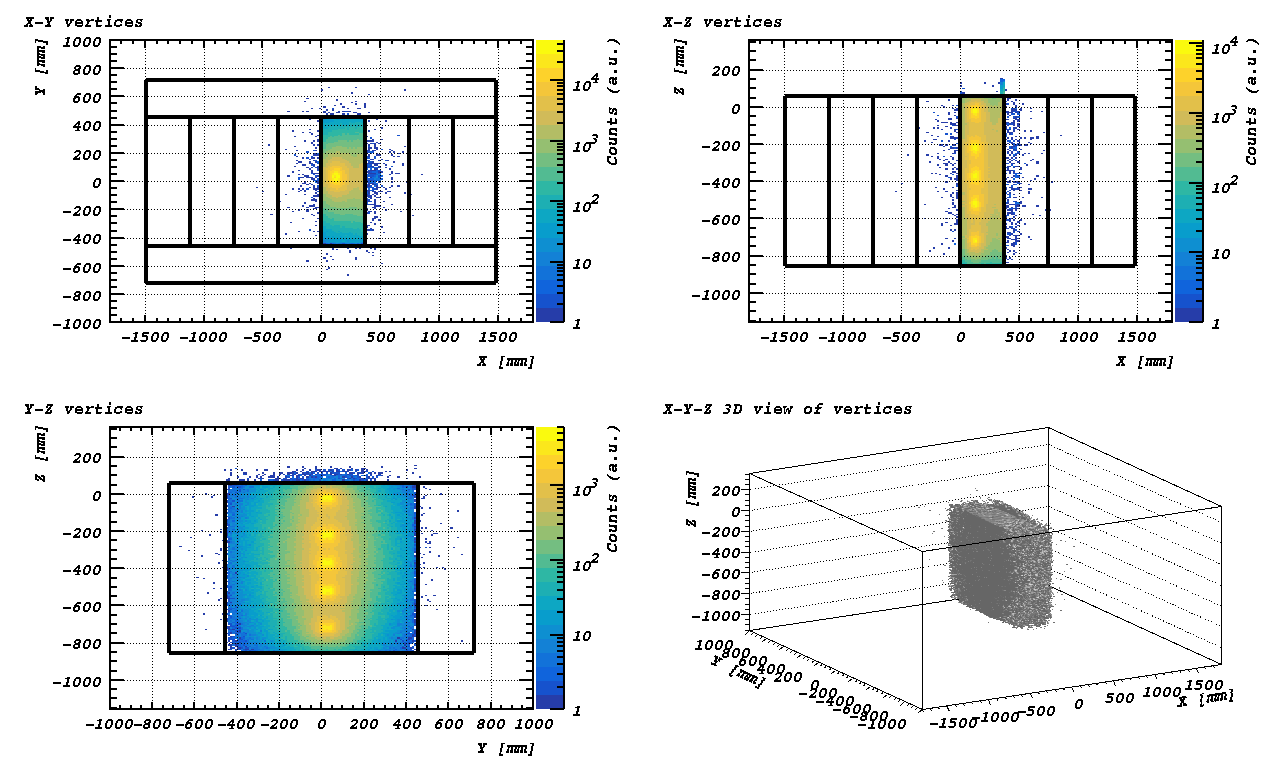
\includegraphics[width=0.99\linewidth]{images/mn_Edep_vertices}
\captionof{figure}{Distribution des premiers vertex d'interaction des gammas du $\ce{^{54}Mn}$ servant à la calibration de la cellule 4. Les sources sont déployées à 5 hauteurs en $z$ rendant les dépôts d'énergies homogènes suivant cet axe. En revanche les valeurs extrêmes en $y$ sont dépeuplées, c'est pourquoi la réponse en énergie a aussi été mise à l'épreuve avec d'autres signaux.}
\label{fig:mn_Edep_vertices}

\end{figure}

\begin{figure}[h!]
\centering

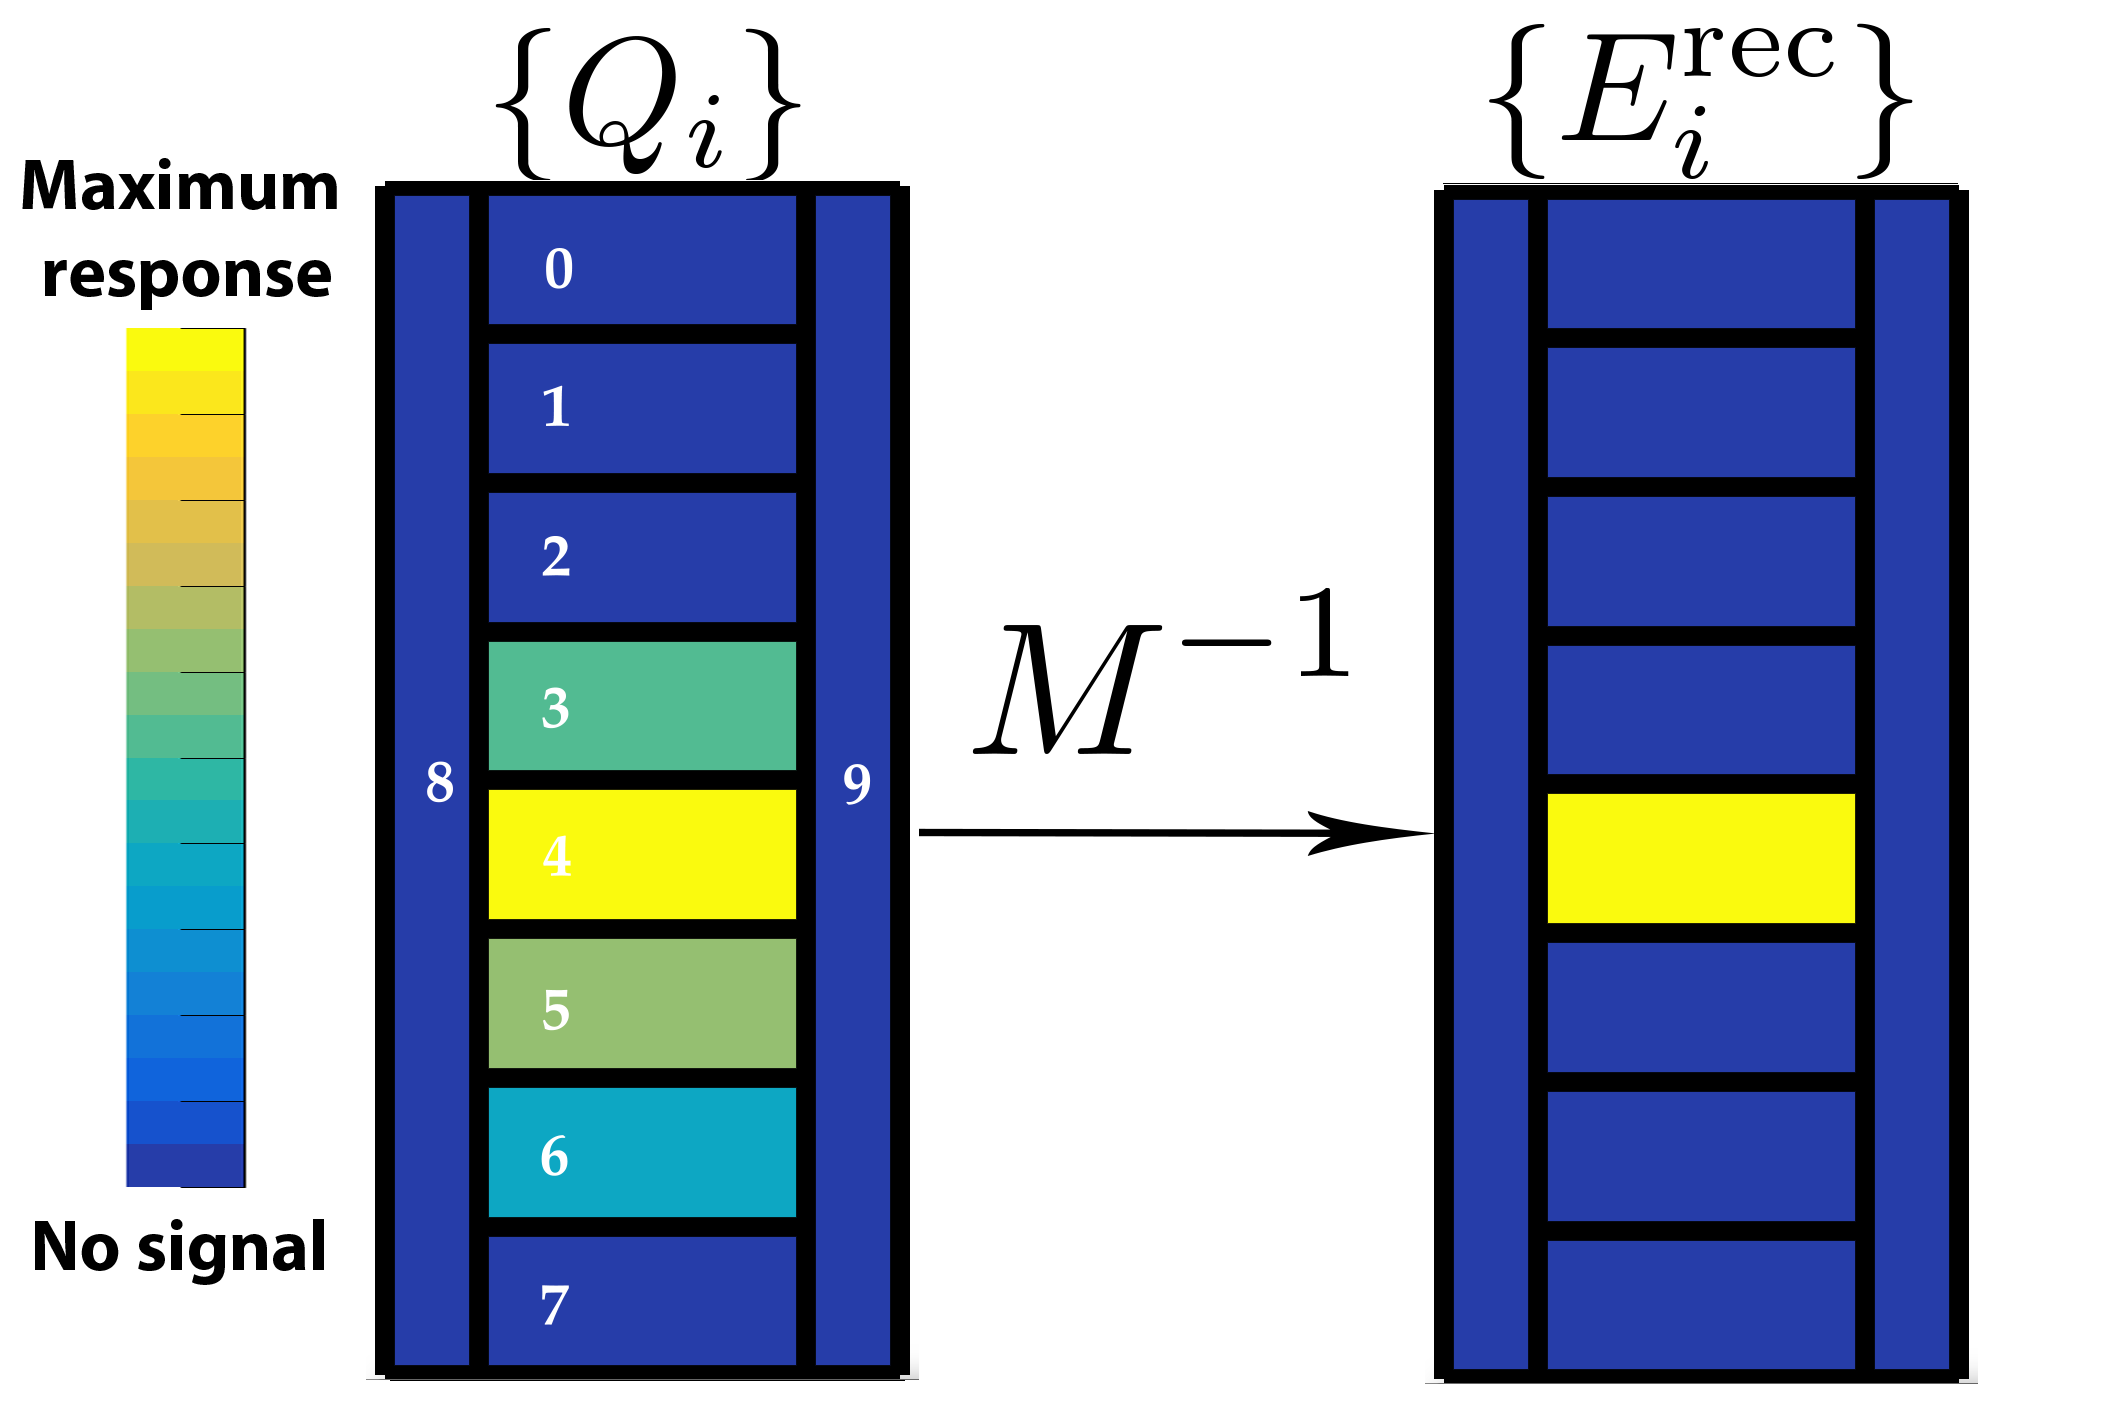
\includegraphics[width=0.8\linewidth]{images/erec_procedure.png}
\captionof{figure}{Représentation de la réponse du détecteur en charge et en énergie reconstruite lors d'un dépôt d'énergie exclusif dans la cellule 4. Les charges collectées dans les cellules voisines à la 4 sont non nulles, alors qu'en énergie reconstruite seule la cellule 4 voit un signal.}
\label{fig:erec_procedure}

\end{figure}

\clearpage
}

%\begin{figure}[h!]
%
%\end{figure}

\bigbreak

\section{Mesure des observables au premier ordre}

\subsection{Les coefficients de calibration}

Comme il a été mentionné précédemment, la calibration a été effectuée avec une source de manganèse 54 ($\ce{^{54}Mn}$). Cette source intense mono gamma à $\SI{835}{keV}$ permet de calibrer le détecteur avec une contribution négligeable de bruit de fond. L'interaction dominante des gammas à cette énergie est la diffusion Compton.\\

Les coefficients de calibration sont obtenus de la même manière dans les données et la simulation. En reprenant la définition des $C_i$, l'équation (\ref{eq:calib_def}) fait intervenir la charge $Q_i$ et l'énergie déposée $E_i^{\textrm{dep}}$. $E_i^{\textrm{dep}}$ ne peut être mesurée directement dans les données, mais cette quantité ne dépend pas des propriétés optiques du détecteur. Le MC fournit donc la valeur de $E_i^{\textrm{dep}}$ utilisée pour déterminer $C_i$ dans les données et la simulation :

\begin{equation}
    C_i = \left<\frac{Q_i}{E_i^{\textrm{dep}}}\right> \simeq \frac{\left<Q_i\right>}{\left<E_i^{\textrm{dep}}\right>},
    \label{eq:calib_def}
\end{equation}

\bigbreak

où la valeur de $\left<Q_i\right>$ doit correspondre à $\left<E_i^{\textrm{dep}}\right>$.  Afin de s'affranchir de la lumière produite dans les cellules voisines, mais contribuant à $\left<Q_i\right>$ via les fuites de lumière, seuls les événements ayant déposé exclusivement de l'énergie dans la cellule $i$ doivent être considérés.\\

La source de $\ce{^{54}Mn}$ est déployée dans les tubes de calibration, mais ces derniers ne sont pas présents dans toutes les cellules : cellules 1, 4 et 6 pendant la phase 1 et 1, 2, 4, 5 et 6 pour la phase 2. Les autres cellules sont en fait calibrées avec les gammas qui n'ont pas interagi avant d'attendre le volume en question. En pratique, les données acquises sont fusionnées et ce sont les coupures topologiques qui permettent de limiter les fuites d'énergie Compton vers les cellules voisines. À l'aide de la valeur centrale des coefficients de fuites de lumière $L_{ij}$ ainsi que de leur dispersion $\Delta L_{ij}$, il est possible de contraindre la charge vue dans les cellules voisines :

\begin{equation}
    \frac{Q_{j \neq i}}{Q_i} < L_{ij} + k\Delta L_{ij}.
\end{equation}

\bigbreak

Une représentation de cette coupure est dessinée figure \ref{fig:Qj_ov_Qi}. La valeur de $k$ est choisie en surveillant qu'un décalage $\delta k$ n'affecte pas (ou très peu) les quantités $\left<Q_i\right>$ et $\left<E_i^{\textrm{dep}}\right>$.\\

Afin d'affiner la justesse des coefficients de calibration, une principale approximation doit être revue. La simulation ne décrit pas parfaitement les propriétés optiques de chaque paroi réfléchissante, alors l'efficacité des coupures anti-Compton est différente entre données et simulation. La correspondance entre $\left<Q_i\right>_{Data}$ et $\left<E_i^{\textrm{dep}}\right>_{MC}$ n'est pas évidente. Un ajustement plus fin des $C_i$ est donc nécessaire. La méthode employée est décrite dans la Section \ref{seq:Erec_tuning}.

\subsection{Les coefficients de fuites de lumière}
\label{sec:LL_JS}

Les fuites de lumière sont mesurées en utilisant les muons cosmiques pendant la prise de données. Leur fort pouvoir pénétrant est exploité pour mesurer des fuites de lumière avec des dépôts d'énergie répartis de façon homogène dans le volume. De plus, les muons qui traversent le détecteur ont un pouvoir ionisant d'environ $\SI{2}{MeV/cm}$ et peuvent déposer jusqu'à plus de $\SI{100}{MeV}$ dans le liquide. Cependant, la linéarité de l'électronique nous impose de rester en deçà de $\SI{40}{MeV}$. Peu d'autres bruits de fond déposent plus de $\SI{20}{MeV}$ dans le détecteur donc la sélection de ces événements est effectuée en appliquant un simple seuil en charge.\\

Pour calibrer les fuites de lumière d'une cellule source $i$, on sélectionne les candidats où la charge est maximum dans cette cellule ($Q_i$) et où la charge totale collectée est supérieure à $\SI{4000}{PE}$ ($\gtrsim \SI{20}{MeV}$). Les distributions de charge $Q_j$ sont stockées dans des histogrammes pour chaque tranche en $Q_i$. Les coefficients $L_{ij}$ sont obtenus en ajustant le coefficient directeur de la droite : $Q_j = L_{ij} Q_i$ (voir figure \ref{fig:LL_JS}). $L_{ij}$ représente en fait la valeur nominale du rapport $Q_j/Q_i$. En pratique des coupures supplémentaires sont imposées pour limiter les fuites d'énergie, ainsi qu'une condition de non-saturation des PMs pour assurer la linéarité de la réponse.\\

%La méthode est présentée en détail dans la note technique de Jean-Sebastien Réal \cite{Real2017}.\\

D'autres techniques ont été développées pour obtenir ces coefficients à partir des runs de $\ce{^{54}Mn}$. Or, si les coefficients $L_{ij}$ peuvent être aisément mesurés dans les cellules possédant un tube de calibration, la procédure est plus délicate pour les autres cellules. Aucune méthode directe avec le $\ce{^{54}Mn}$ n'a donné de résultat satisfaisant pour reconstruire l'énergie. Finalement, ce sont les coefficients $L_{ij}$ mesurés à partir des cosmiques qui sont utilisés au premier ordre et l'énergie reconstruite est ajustée plus finement avec les runs de calibration en corrigeant les paramètres $C_i$ et $L_{ij}$ itérativement. La procédure est décrite dans la section suivante.\\

\afterpage{%

\begin{figure}[h!]
  \centering
  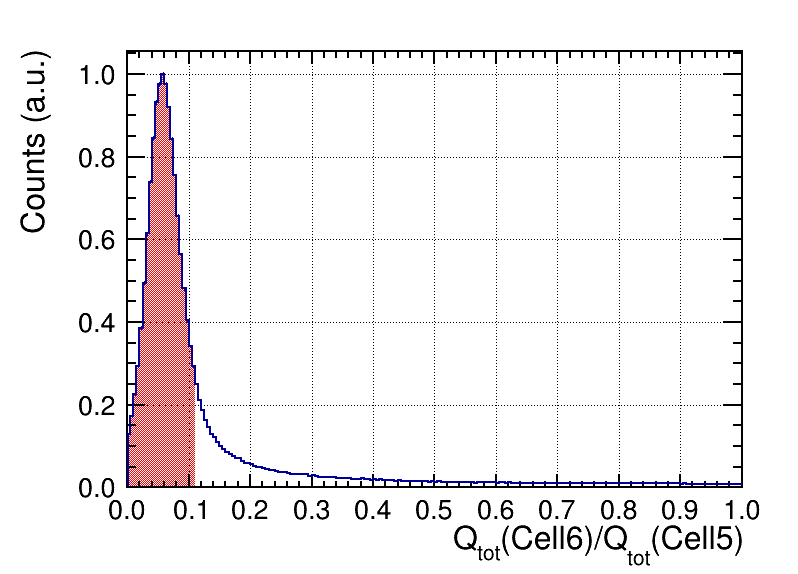
\includegraphics[width=0.75\linewidth]{images/Qj_ov_Qi.png}
  \captionof{figure}{Distribution des rapports de charge $Q_j/Q_i$ (j = Cellule 6 et i = Cellule 5). La source de $\ce{^{54}Mn}$ est disposée dans la cellule 5 ($i$), et cette distribution sert à ajuster les fuites de lumière de $i$ vers $j$ : $L_{ij}$. La zone en rouge représente les événements sélectionnés pour la calibration.}
  \label{fig:Qj_ov_Qi}
\end{figure}

\begin{figure}[h!]
  \centering
  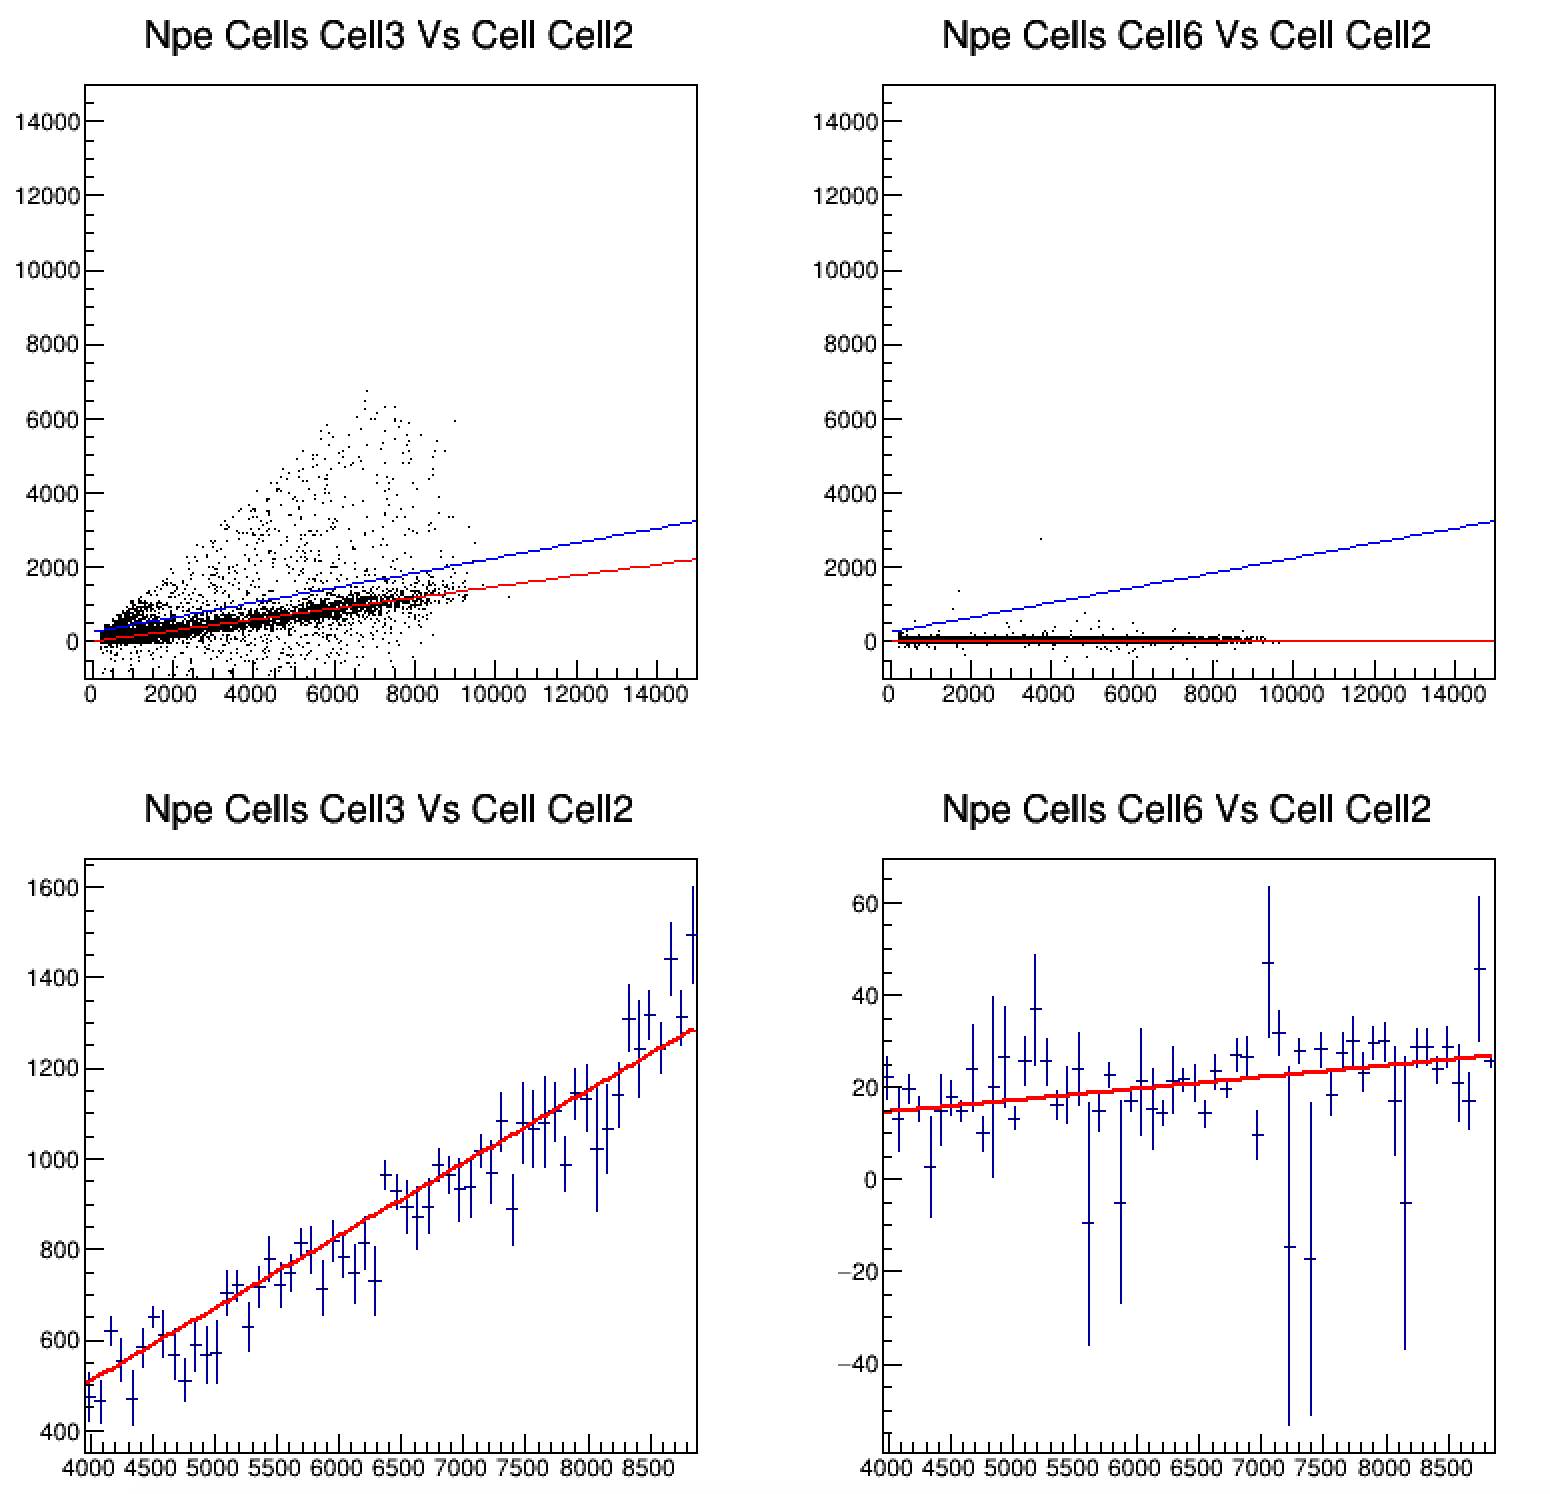
\includegraphics[width=0.75\linewidth]{images/LL_JS.png}
  \caption[Mesure des coefficients de fuites de lumière $L_{ij}$ avec les muons cosmiques]{Mesure des coefficients de fuites de lumière $L_{ij}$ avec les muons cosmiques. À droite la charge collectée dans la cellule 6 contre celle dans la cellule 2. À gauche la charge dans la cellule 3 contre la cellule 2. Les événements sous les lignes bleues sont utilisés pour remplir un graph profilé (figure en bas) sur lequel est ajusté une droite (en rouge) pour obtenir les fuites de lumière. (source : \cite{docdb165})}
  \label{fig:LL_JS}
\end{figure}

\clearpage
}

\section{Ajustement des paramètres de collection de lumière}

L'ajustement des paramètres de collection de lumière est une procédure itérative qui vise à harmoniser la valeur la plus probable des énergies reconstruites dans la simulation ($E^{\textrm{rec}}_{\textrm{MC}}$) et dans les données ($E^{\textrm{rec}}_{\textrm{Data}}$) sur une référence commune $E^{\textrm{ref}}$. Après avoir présenté les coupures nécessaires, cette section décrit la façon dont les énergies de référence sont établies, et ensuite la procédure d'ajustement des $C_i$ et $L_{ij}$. Enfin, l'évaluation des erreurs systématiques liées à cet ancrage est présentée.

\subsection{Coupures utilisées}
\label{sec:cuts_for_Erec_tuning}

Un des avantages de l'ajustement itératif des $C_i$ et $L_{ij}$ est de pouvoir utiliser des coupures sur les énergies reconstruites elles-mêmes. De telles coupures peuvent donc être utilisées dans les données et la simulation tout en étant indépendantes des paramètres optiques au premier ordre.\\

Bien que la source de $\ce{^{54}Mn}$ soit très intense, les cellules qui ne possèdent pas de tube de calibration sont calibrées avec une quantité de gammas sensiblement plus faible. En effet, les gammas ne doivent pas  interagir avant d'avoir atteint la cellule en question. La statistique est drastiquement réduite notamment pour les longues cellules du Gamma Catcher. Les bruits de fond d'origine cosmique et la radioactivité naturelle des matériaux environnants n'étant plus négligeables devant le signal $\ce{^{54}Mn}$, ils doivent être retirés. Pour ce faire, les coupures suivantes sont appliquées dans les données :

\begin{itemize}
    \item[$\bullet$] Charge dans le véto muon $Q_{veto} < \SI{80}{pe}$,
    \item[$\bullet$] Temps depuis le dernier événement d'origine cosmique $\Delta T_\mu > \SI{30}{\mu s}$.
\end{itemize}

\bigbreak

Pour ajuster les coefficients de calibration, les événements doivent avoir déposé toute leur énergie dans la cellule $i$. Les conditions suivantes sont imposées dans les données comme dans le MC :

\begin{itemize}
    \item[$\bullet$] La cellule ayant reconstruit le maximum d'énergie doit être $i$,
    \item[$\bullet$] Les énergies reconstruites dans toutes les autres cellules doivent être inférieures à $\SI{100}{keV}$ (anti-Compton) : $E^{\textrm{rec}}_{j\neq i} < \SI{0.1}{MeV}$.
\end{itemize}

\bigbreak

En principe les fuites de lumière peuvent être ajustées dans les mêmes conditions, car la coupure anti-Compton limite suffisamment  les partages d'énergie. Cependant, les cellules adjacentes à $i$ ont en moyenne une part de fuites d'énergie non négligeable. Afin de contrôler le biais sur la mesure des fuites de lumière, d'autres critères de sélection sont utilisés pour ajuster $L_{ij}$ :

 \begin{itemize}
    \item[$\bullet$] La cellule ayant reconstruit le maximum d'énergie doit être $i$,
    \item[$\bullet$] La cellule $i$ doit au moins contenir $\SI{60}{\%}$ de l'énergie totale reconstruite : $E^{\textrm{rec}}_{i} > 0.6E^{\textrm{rec}}_{tot}$,
    \item[$\bullet$] La seconde cellule ayant reconstruit le maximum d'énergie doit être $j$ (pour contrôler que les fuites d'énergie Compton ont lieu dans $j$, et ainsi ajuster correctement $L_{ij}$),
    \item[$\bullet$] L'énergie reconstruite dans les autres cellules doit être inférieure à $5 \%$ du total.\\
\end{itemize}

Même si les coefficients $C_i$ et $L_{ij}$ ne sont pas parfaitement ajustés lorsque les coupures sur l'énergie reconstruite sont sollicitées, la population d'événements sélectionnée est suffisamment pure pour faire converger les paramètres après quelques itérations.\\

\subsection{Détermination des énergies de référence}

La construction d'énergies de référence est cruciale, car ce sont elles qui assurent que toutes les cellules donnent une réponse en énergie similaire. La simulation procure la vraie quantité d'énergie déposée dans le liquide pour chaque cellule. En revanche, la valeur la plus probable de l'énergie reconstruite ne peut pas être directement comparée à celle de l'énergie déposée, car des gammas n'ayant pas tout déposé affectent la distribution d'énergie reconstruite (voire figure \ref{fig:erec_vs_edep}). Pour effectuer une comparaison cohérente, l'énergie déposée donnée par la simulation doit être convoluée par une fonction de réponse imitant celle du détecteur. Deux méthodes ont été testées : la \og convolution gaussienne\fg{} et la \og convolution patchwork\fg{}.\\

\afterpage{%

\begin{figure}[p]
  \centering
  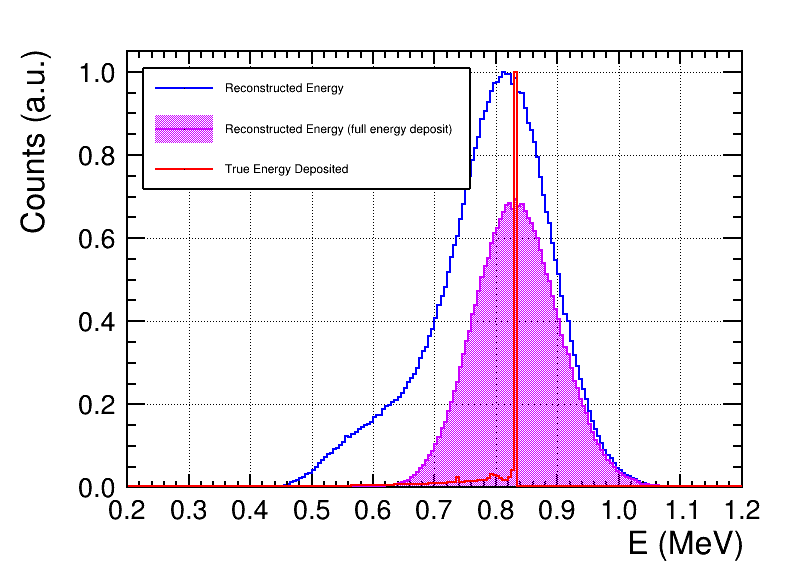
\includegraphics[width=0.8\linewidth]{images/erec_vs_edep}
  \caption[Évolution de la position de la valeur la plus probable en énergie reconstruite en fonction des événements considérés]{Évolution de la position de la valeur la plus probable en énergie reconstruite en fonction des événements considérés. La valeur la plus probable de la distribution avec tous les événements (bleu) se retrouve légèrement décalée vers les basses énergies par rapport à celle où seuls les gammas qui ont tout déposé dans le liquide sont considérés (violet). La valeur la plus probable de la distribution en bleu ne coïncide donc pas avec le pic d'énergie totale déposée (rouge). Cet effet justifie l'utilisation de méthodes de convolution des énergies déposées pour construire des points d'ancrage $E^\textrm{ref}$ sur lesquels les distributions d'énergie reconstruite doivent s'aligner.}
  \label{fig:erec_vs_edep}
\end{figure}

\clearpage
}

À énergie déposée fixe, la réponse en énergie reconstruite suit une loi de gauss en première approximation. La procédure de convolution gaussienne vise à construire une distribution d'énergie dite \og convoluée \fg{} en appliquant sur chaque événement un décalage sur l'énergie déposée :

\begin{equation}
    E^{\textrm{conv}}_{i} = E^{\textrm{dep}}_{i} + \delta E(\sigma_i),
\end{equation}

\bigbreak

où $\delta E$ est une variable aléatoire suivant une loi gaussienne de largeur $\sigma_i$. $\sigma_i$ est obtenu en prenant la déviation standard de la distribution d'énergie reconstruite (avec des paramètres au premier ordre) des événements ayant laissé toute leur énergie dans le liquide (voir distribution violette, figure \ref{fig:erec_vs_edep}). Elle est considérée comme constante bien que la résolution varie avec la quantité d'énergie déposée. Cette approximation est acceptable dans la mesure où la valeur attendue de $E^{\textrm{ref}}$ est proche de l'énergie nominale. La figure \ref{fig:E_conv_vs_E_rec} montre que la distribution d'énergies convoluées a une forme très similaire à la réponse du détecteur dans la région du maximum. La déviation croissante à basse énergie vient du fait que la distribution en énergie reconstruite est coupée à $\SI{0.5}{MeV}$. L'effet sur la distribution convoluée est similaire à celui de la convolution d'une porte par une gaussienne : la marche est adoucie. L'énergie de référence est mesurée en ajustant une courbe gaussienne autour de la valeur la plus probable ($\pm \SI{100}{keV}$). Le paramètre $\mu$ de la gaussienne est pris comme $E^{\textrm{ref}}$.\\

 Sur la figure \ref{fig:E_conv_vs_E_rec}, on peut observer que l'écart entre énergies reconstruites et convoluées présente néanmoins une pente résiduelle dans la région du maximum. Cette déviation induit un biais sur l'extraction de $E^{\textrm{ref}}$ à hauteur de $0.1\%$. Le principal candidat provoquant cet effet est l'approximation gaussienne de la réponse du détecteur. Les effets de volume dans les coins des cellules affectent l'efficacité de collection de la lumière, donc le modèle de réponse gaussienne doit être amélioré. C'est l'objet de la \og convolution par patchwork\fg{}, qui utilise la véritable forme de la réponse en énergie reconstruite.\\

 Dans la convolution par patchwork, la forme de la réponse en énergie reconstruite est extraite en isolant les événements issus de chaque bins en énergie déposée. Pour ce faire, des coefficients $C_i$ et $L_{ij}$ au premier ordre sont exploités. Chaque distribution extraite en $E^\textrm{rec}$ est recalée de telle manière à ce que la moyenne corresponde à celle du bin en énergie déposée $E^\textrm{dep}$. Les distributions recalées sont ensuite superposées dans un histogramme commun. Enfin, une gaussienne est ajustée par-dessus cet histogramme afin d'extraire $E^{\textrm{ref}}$ comme précédemment. La figure \ref{fig:E_patch_vs_E_rec} montre finalement que la convolution par patchwork est en meilleur accord avec l'énergie reconstruite.\\

\afterpage{%

\begin{figure}[h!]
  \centering
  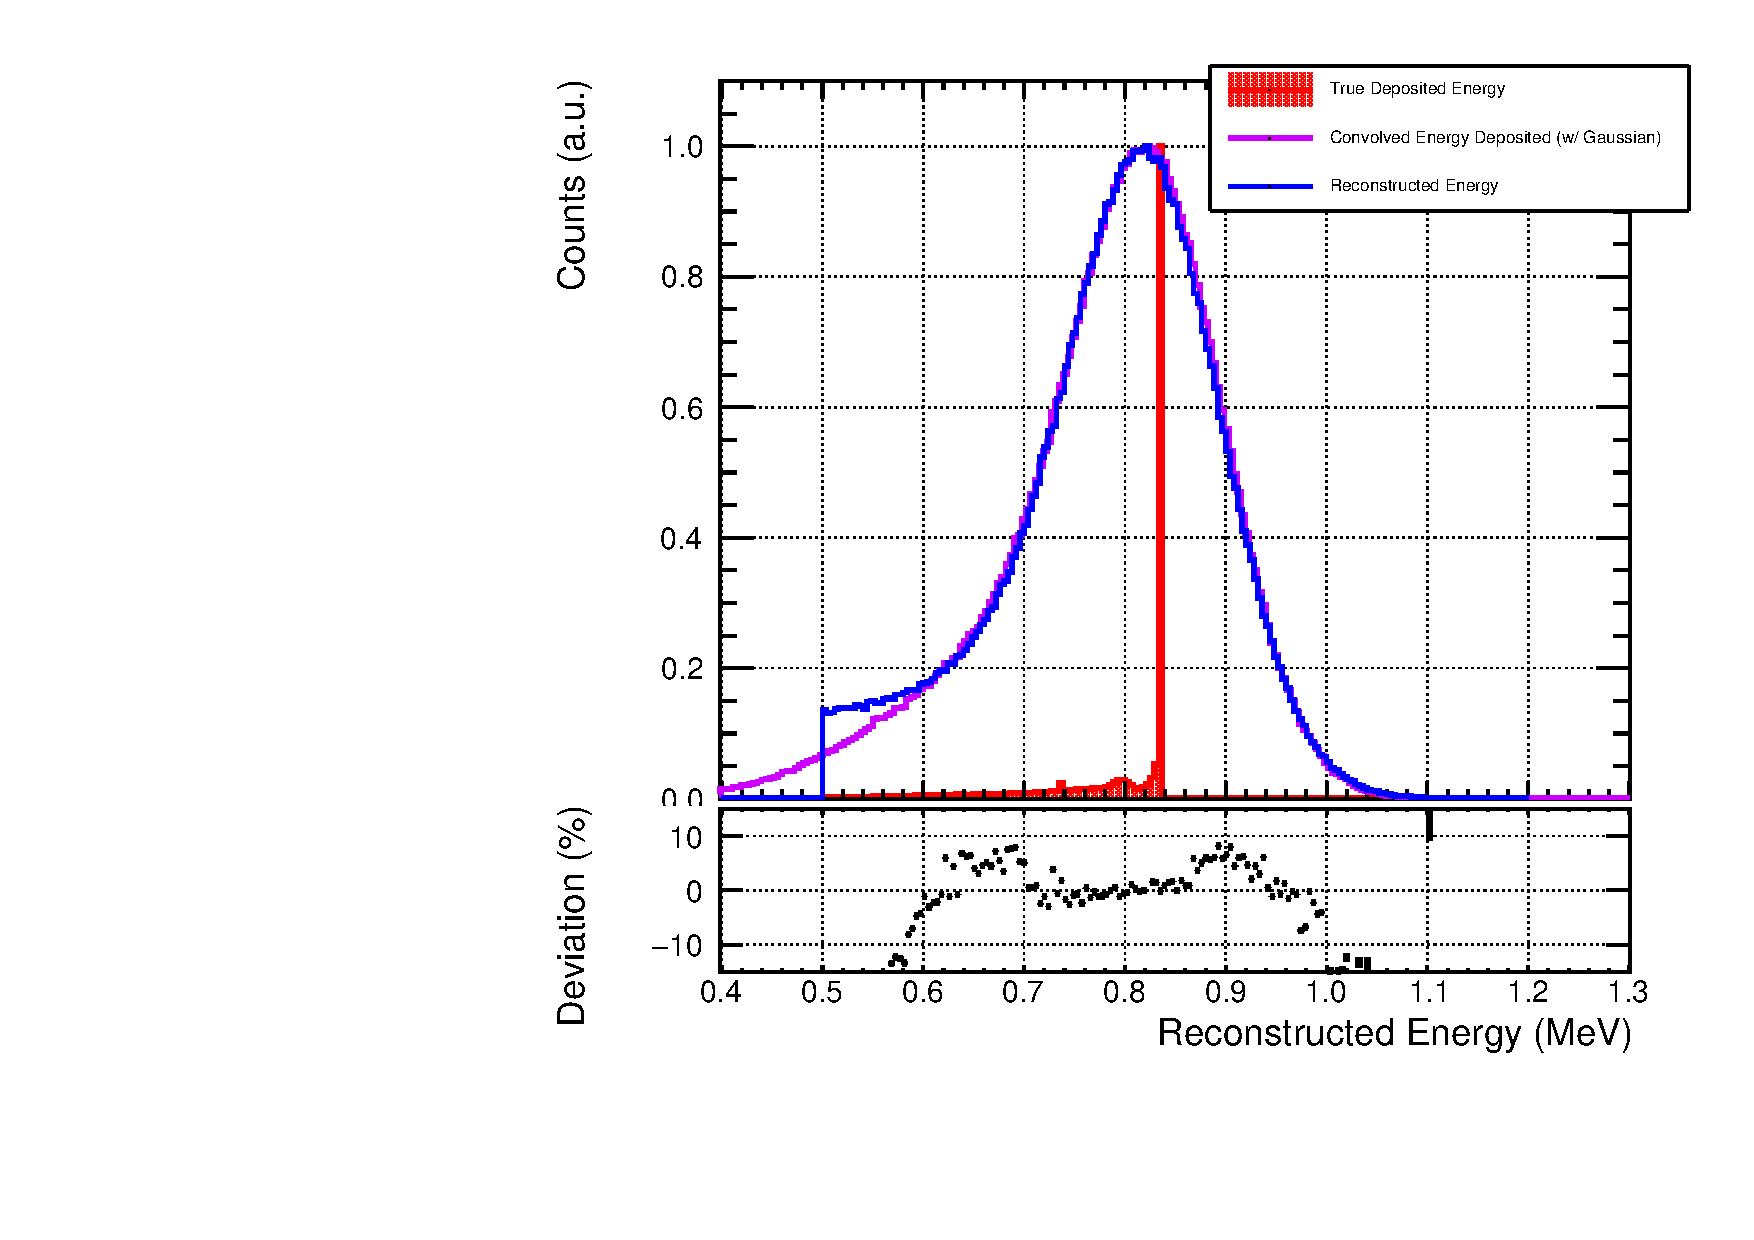
\includegraphics[width=0.7\linewidth]{images/E_conv_vs_E_rec_gaussian.pdf}
  \caption[Comparaison entre la distribution d'énergie par convolution gaussienne et l'énergie reconstruite]{Comparaison entre la distribution d'énergie par convolution gaussienne (violet) et l'énergie reconstruite (bleu) obtenues dans la simulation. Pour pouvoir comparer la forme des deux distributions, l'énergie reconstruite a été ajustée au préalable. La déviation relative est présentée en dessous (noir). L'histogramme en rouge représente la distribution d'énergie déposée dans le liquide. }
  \label{fig:E_conv_vs_E_rec}
\end{figure}

\begin{figure}[h!]
  \centering
  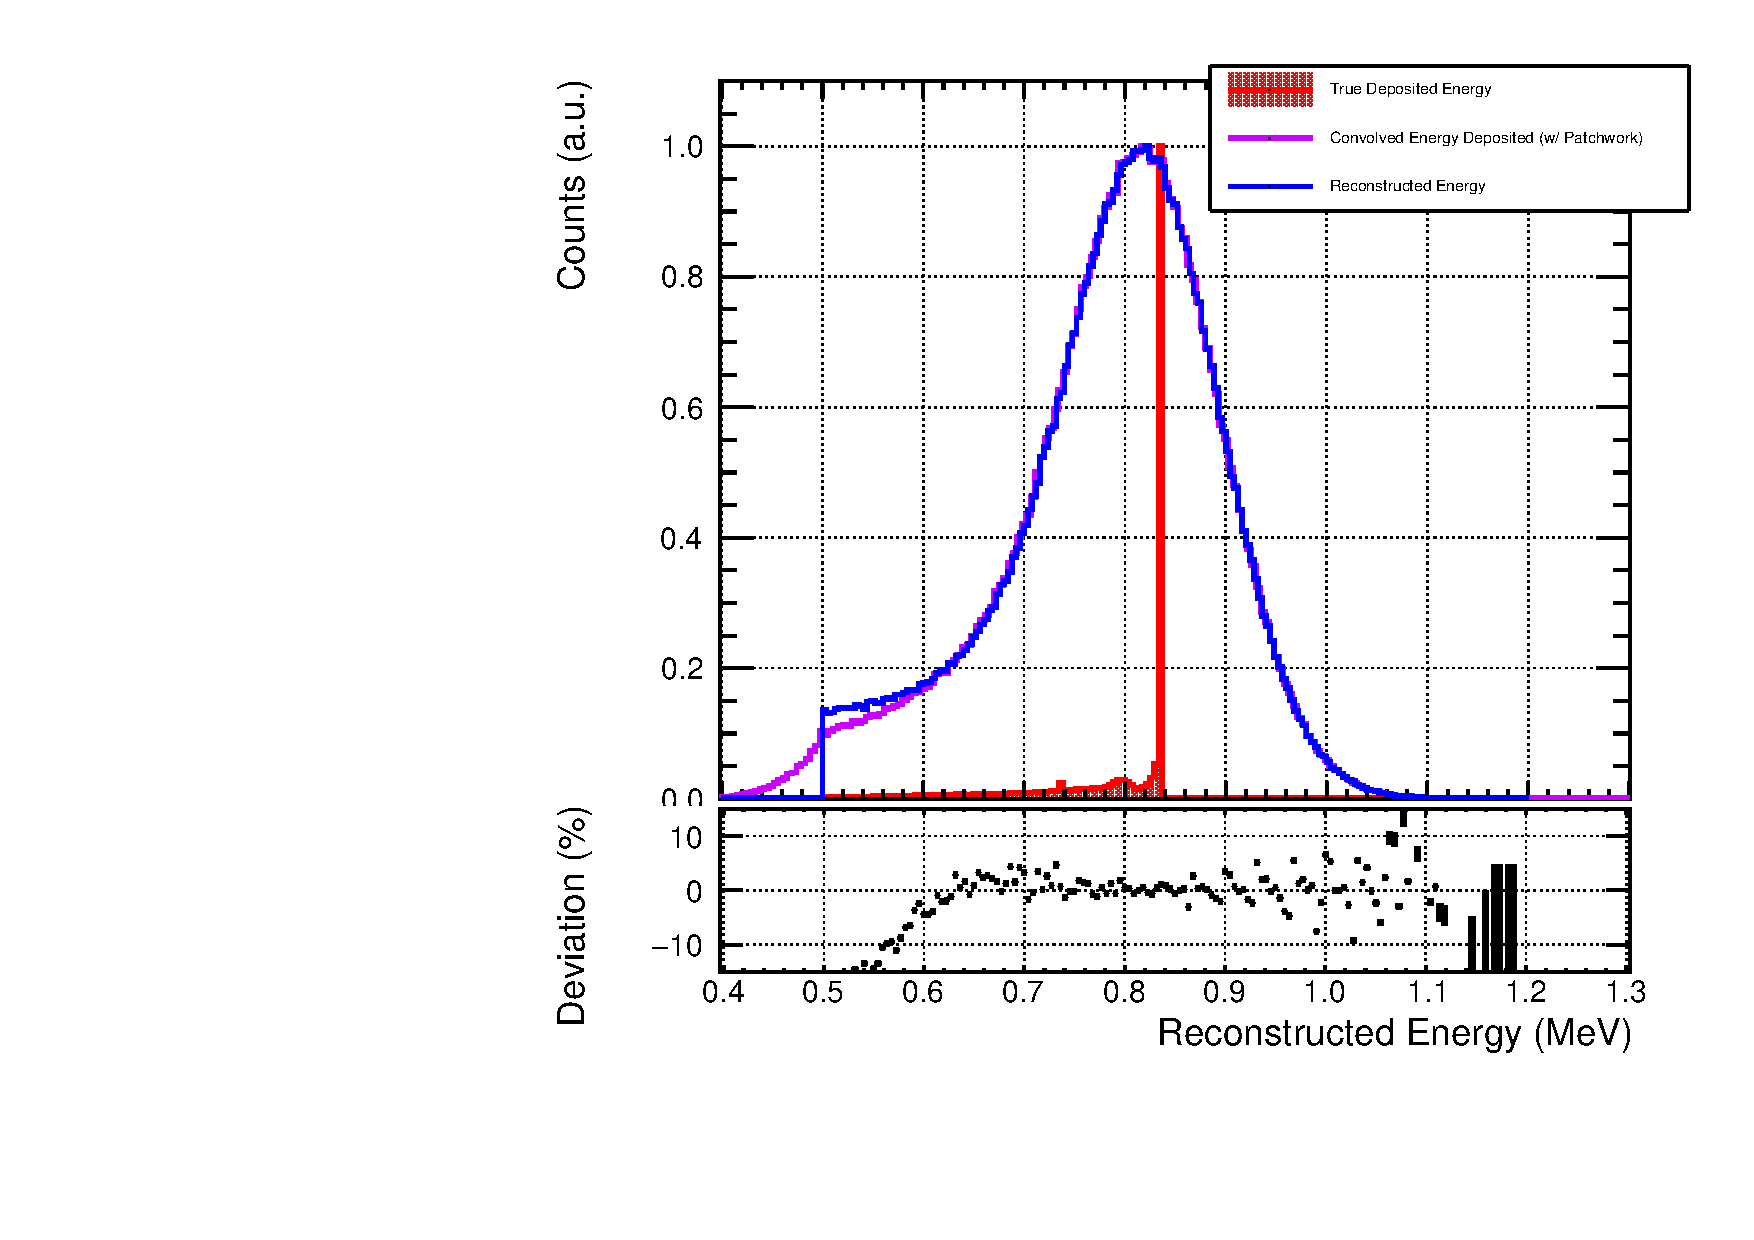
\includegraphics[width=0.7\linewidth]{images/E_conv_vs_E_rec_patchwork.pdf}
  \caption[Comparaison entre la distribution d'énergie convolution par patchwork et l'énergie reconstruite]{Comparaison entre la distribution d'énergie convolution par patchwork (violet) et l'énergie reconstruite (bleu) obtenues dans la simulation. Pour pouvoir comparer la forme des deux distributions, l'énergie reconstruite a été ajustée au préalable. La déviation relative est présentée en dessous (noir). L'histogramme en rouge représente la distribution d'énergie déposée dans le liquide.}
  \label{fig:E_patch_vs_E_rec}
\end{figure}

\clearpage
}

Ces procédures de convolution sont répétées pour fournir une énergie de référence à chaque set de coupures utilisées. Il y a donc autant de $E^\textrm{ref}$ que de $C_i$ et $L_{ij}$ combinés. La correspondance entre énergies reconstruites et paramètres de collection de lumière est explicitée dans la section suivante. Les deux méthodes de convolution donnent des résultats similaires à $\pm \SI{0.2}{\%}$ près. Ce chiffre est retenu comme incertitude sur chaque $E^{\textrm{ref}}$. En pratique, les valeurs $E^{\textrm{ref}}$ fournies par la convolution patchwork sont utilisées pour l'ajustement des $C_i$ et $L_{ij}$.\\

\subsection{Correction itérative des paramètres de collection de lumière}
\label{seq:Erec_tuning}

Les dépôts d'énergie gamma du $\ce{^{54}Mn}$ sont suffisamment localisés pour ne considérer que deux cellules. L'\'Equation \ref{eq:qtot_expression} peut donc être simplifiée en réduisant la dimension de la matrice M à $2\times 2$. Dans ce cas, elle peut être facilement inversée :

\begin{equation}
    \label{eq:Erec_2_by_2_case}
  \left(
  \begin{matrix}
  E_1 \\
  E_2
  \end{matrix}\right)
 = \frac{\left(
  \begin{matrix}
    C_2 & -C_2L_{21} \\
    -C_1L_{12} & C_1
  \end{matrix}\right) \left(
  \begin{matrix}
    Q_1 \\
    Q_2
  \end{matrix}\right)}
  {C_1C_2(1 - L_{12}L_{21})},
\end{equation}

\bigbreak

où l'indice $1$ désigne la cellule ayant reçu le plus d'énergie, et $2$ la cellule contenant d'éventuelles fuites d'énergie. Au premier ordre, le décalage en énergie reconstruite $\delta E_1 \doteq E_1^{\textrm{ref}} - E_1^{\textrm{rec}}$ peut être exprimé en fonction de $\delta C_1 \doteq C_1^{\textrm{ref}} - C_1^{\textrm{rec}}$ et $\delta L_{12} \doteq L_{12}^{\textrm{ref}} - L_{12}^{\textrm{rec}}$ où $C_1^{\textrm{rec}}$ et $L_{12}^{\textrm{rec}}$ sont les paramètres utilisés pour reconstruire $E_1^{\textrm{rec}}$, et $C_1^{\textrm{ref}}$ et $L_{12}^{\textrm{ref}}$ les paramètres de références qui permettent d'obtenir $E_1^{\textrm{ref}}$ :

\begin{equation}
    \label{eq:dE_step}
  \delta E_1 = \frac{Q_1\left\{
  \frac{\delta C_1}{C_1^{\textrm{rec}}} - \frac{Q_2L_{12}^{\textrm{rec}}}{Q_1}\left(\frac{\delta C_1}{C_1^{\textrm{rec}}} + \frac{\delta L_{12}}{L_{12}^{\textrm{rec}}}\right)\right\}}{(1 - L^{\textrm{rec}}_{12}L^{\textrm{rec}}_{21})C_1^{\textrm{rec}}}
  + \mathcal{O}\left[
        \left(\frac{\delta C_1}{C_1^{\textrm{rec}}}\right)^{2}
        , \frac{\delta C_1}{C_1^{\textrm{rec}}}\frac{\delta L_{12}}{L_{12}^{\textrm{rec}}}
    \right].
\end{equation}

\bigbreak

Puisque nous avons considéré que l'énergie est principalement déposée dans $1$ ($E_1^{\textrm{rec}} \gg E_2^{\textrm{rec}}$), le facteur $Q_2L_{12}^{\textrm{rec}}/Q_1$ est négligeable. Ainsi, le biais de calibration $\delta C_1$ au premier ordre peut être exprimé en inversant l'\'Equation \ref{eq:dE_step} :

\begin{equation}
\label{eq:delta_C}
  \delta C_1 =  -\frac{\delta E_1}{E_1^{\textrm{rec}}}C_1^{\textrm{rec}}(1 - L_{12}^{\textrm{rec}}L_{21}^{\textrm{rec}}).
\end{equation}

\bigbreak

De la même manière, l'erreur sur le coefficient de fuites de lumière peut être exprimée en fonction de $\delta E_2$ :

\begin{equation}
  \delta E_2 = \frac{- E_1^{\textrm{rec}}C_1^{\textrm{rec}}\delta L_{12}}{(1 - L_{12}^{\textrm{rec}}L_{21}^{\textrm{rec}})C_2^{\textrm{rec}}}
  + \mathcal{O}\left[
    \left(\frac{\delta C_2}{C_2^{\textrm{rec}}}\right)^{2},
    \left(\frac{\delta L_{12}}{L_{12}^{\textrm{rec}}}\right)^{2},
    \frac{\delta C_2}{C_2^{\textrm{rec}}}\frac{\delta L_{12}}{L_{12}^{\textrm{rec}}}
  \right],
\end{equation}

\begin{equation}
  \label{eq:delta_L}
  \delta L_{12} = - \frac{\delta E_2}{E_1^{\textrm{rec}}}\frac{C_2^{\textrm{rec}}}{C_1^{\textrm{rec}}}(1 - L_{12}^{\textrm{rec}}L_{21}^{\textrm{rec}}).
\end{equation}

\bigbreak

\afterpage{
% iteration_factor.pdf
\begin{figure}[h!]
  \centering
  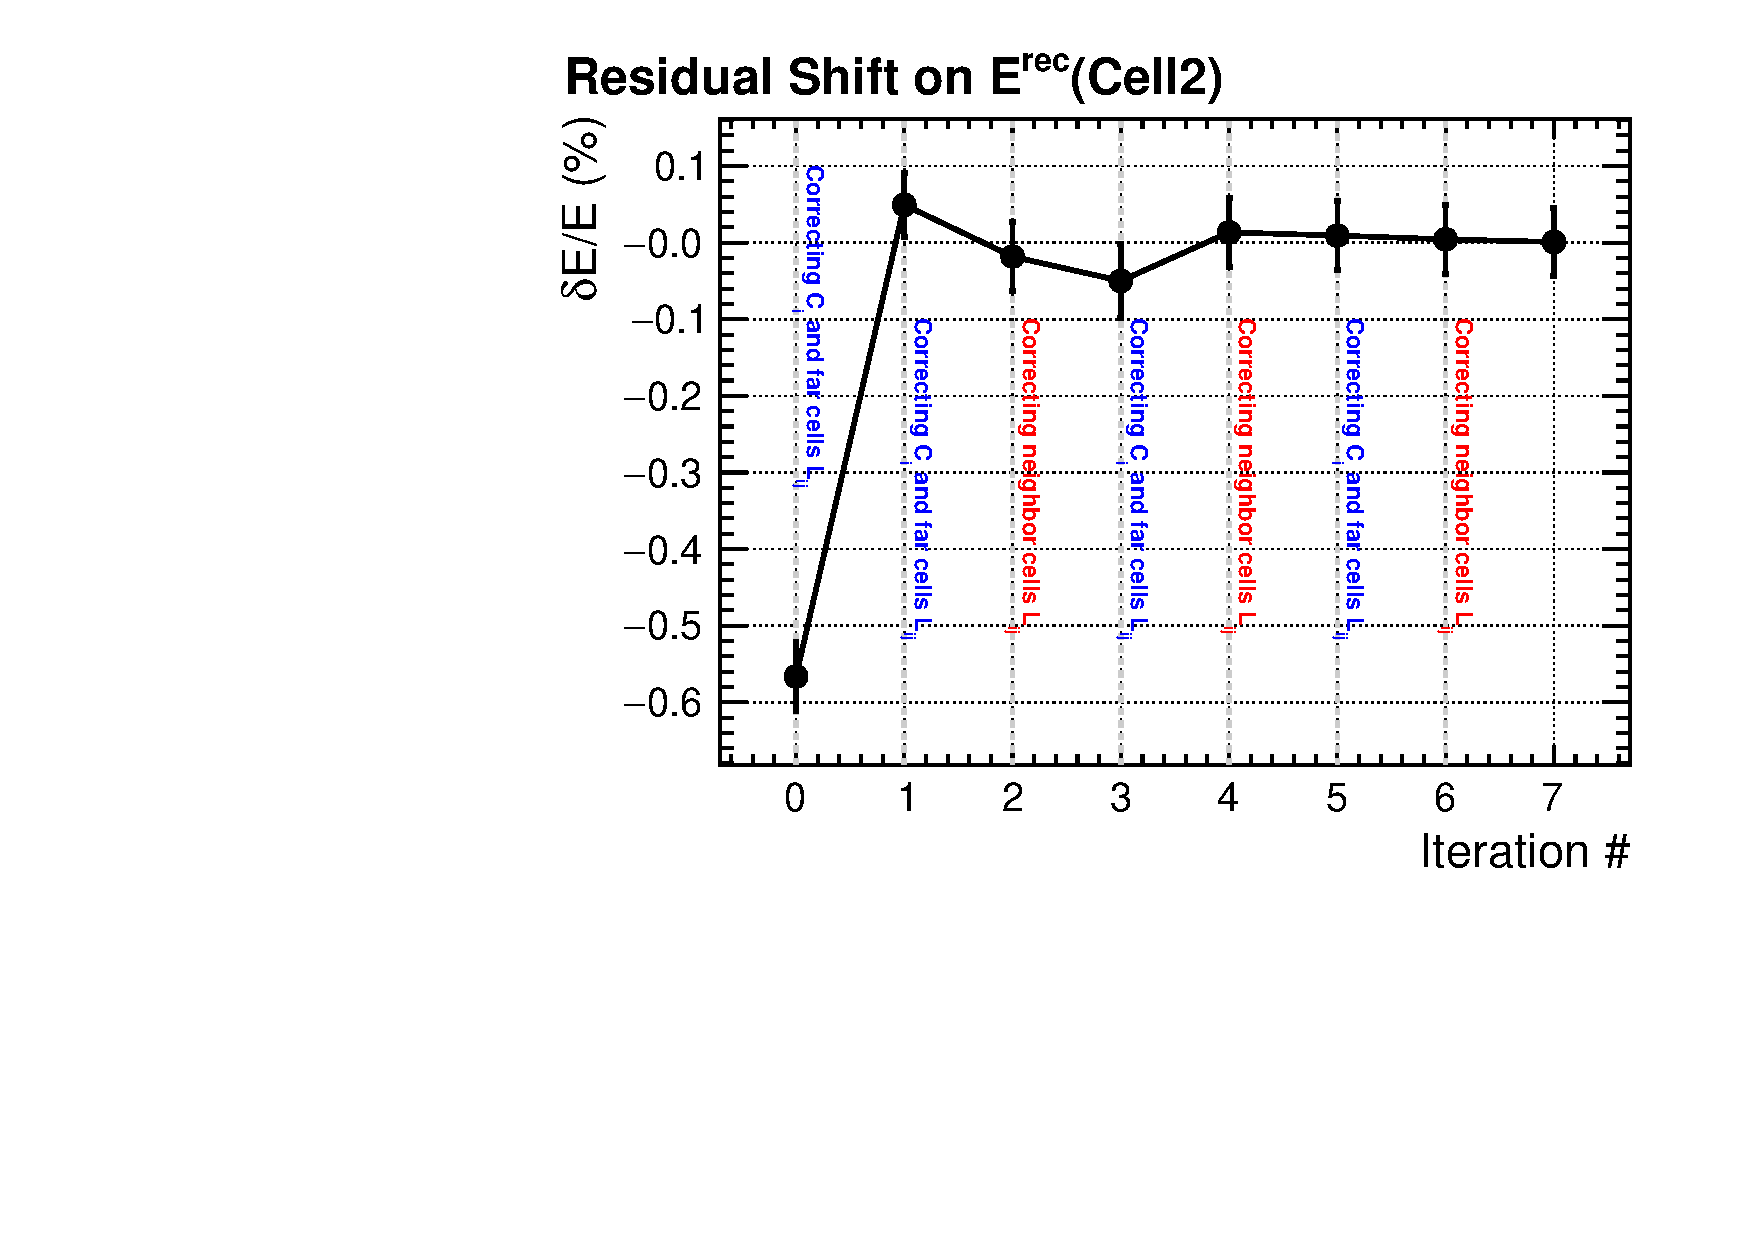
\includegraphics[width=0.8\linewidth]{images/iteration_factor.pdf}
  \caption[Application itérative des corrections sur les $C_i$ et $L_{ij}$]{Application itérative des corrections sur les $C_i$ et $L_{ij}$. Les deux premières itérations sont dédiées aux corrections sur les $C_i$ et $L_{ij}$ des cellules lointaines, et à partir de l'itération $\textrm{n}^{\circ}$ 2, les corrections sur les $L_{ij}$ des cellules voisines sont appliquées en alternance. L'ajustement des $C_i$ et $L_{ij}$ des cellules lointaines diminuent le décalage $\delta E_1$ (Éq. \ref{eq:delta_C}) alors que l'ajustement sur $L_{ij}$ des cellules voisines affecte le décalage $\delta E_{tot}$ (\ref{eq:dE_full}).}
\label{fig:iteration_factor.pdf}
\end{figure}

}

%Les inhomogénéités de fuites de lumière dans le volume des cellules nous empêche d'utiliser directement l'\'Equation \ref{eq:delta_L} pour les cellules adjacentes. En effet, si un dépôt d'énergie a lieu dans un coin d'une cellule où la fuite lumière est amplifiée, une partie de la lumière n'est pas considérée puisqu'elle s'est échappée.

Lorsque les cellules 1 et 2 sont voisines, il reste difficile de séparer les fuites d'énergie probables des fuites de lumière. L'astuce pour contourner cette difficulté consiste à regarder l'énergie reconstruite dans l'ensemble du détecteur ($E^{\textrm{rec}}_{tot} \doteq \sum_{i = \textrm{cells}} E^\textrm{rec}_i$) une fois que tous les autres coefficients sont ajustés. Ainsi, le biais résiduel sur $E^{\textrm{rec}}_{tot}$ est corrigé en ajustant la fuite de lumière adjacente $\delta L_{12}$ :

\begin{equation}
\label{eq:dE_full}
  \frac{\delta E_{tot}}{E^{\textrm{rec}}_1} \simeq - \frac{\delta L^{\textrm{rec}}_{12}C^{\textrm{rec}}_1}{(1 - L^{\textrm{rec}}_{12}L^{\textrm{rec}}_{21})C^{\textrm{rec}}_2},
\end{equation}

\begin{equation}
\label{eq:dL_full_vanilla}
  \delta L_{12} = - \frac{\delta E_{tot}}{E_1^{\textrm{rec}}}\frac{C_2^{\textrm{rec}}}{C_1^{\textrm{rec}}}(1 - L_{12}^{\textrm{rec}}L_{21}^{\textrm{rec}}).
\end{equation}

\bigbreak

Ces corrections sont appliquées itérativement jusqu'à ce que les résidus $\delta E_{tot}$ et $\delta E_1$ deviennent négligeables. Les valeurs de $E^{\textrm{rec}}$ sont évaluées de la même manière que les énergies de référence $E^{\textrm{ref}}$ : en ajustant une courbe gaussienne autour de la valeur la plus probable. En pratique, seuls les coefficients de calibration $C_i$ et de fuites de lumière $L_{ij}$ non adjacentes sont corrigés à l'aide des \'Equations (\ref{eq:delta_C}) et (\ref{eq:delta_L}) pendant les deux premières itérations. Ensuite, l'\'Equation (\ref{eq:dL_full_vanilla}) est sollicitée pour ajuster les fuites de lumière adjacentes une itération sur deux. Un schéma qui résume le déroulement des corrections est présenté sur la figure \ref{fig:iteration_factor.pdf}. La procédure d'ajustement s'arrête lorsque $\delta E_1$ et $\delta E_{tot}$ ont tous les deux convergé.\\

L'ajustement des paramètres de collection de lumière a permis d'établir un accord très satisfaisant entre l'énergie reconstruite dans la simulation et les données (voir figure \ref{fig:Erec_MC_vs_Data}). Les résidus de l'énergie reconstruite entre données et simulation sont tous inclus dans une bande de $\pm 0.2 \%$ pour les cellules de la Target et $\pm 0.4 \%$ pour les cellules du GammaCatcher (voir figure \ref{fig:Erec_vs_anchor_vs_time}).\\

\afterpage{

\begin{figure}[h!]
  \centering
  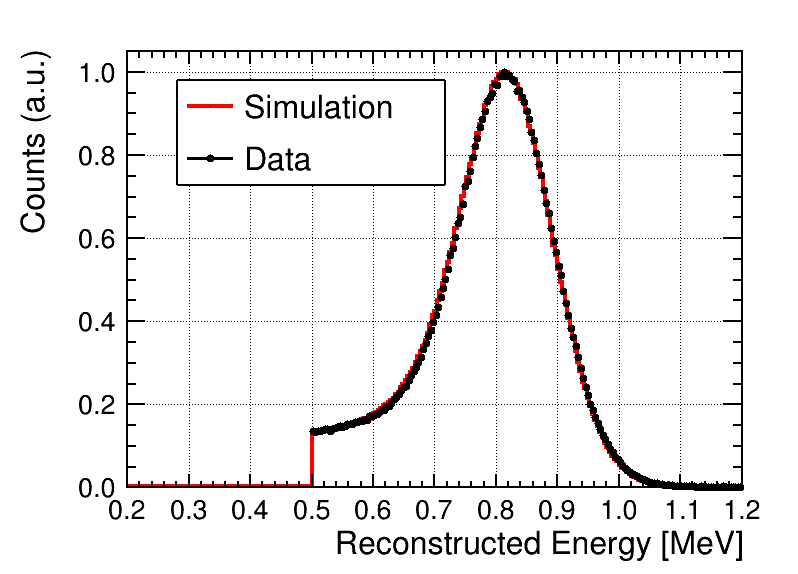
\includegraphics[width=0.85\linewidth]{images/Erec_MC_vs_Data.png}
  \caption[Comparaison des distributions en énergie reconstruite dans les données et la simulation après ajustement des paramètres de collection de lumière]{Comparaison des distributions en énergie reconstruite dans les données (noir) et la simulation (rouge) après ajustement des paramètres de collection de lumière. La marche à $\SI{500}{keV}$ correspond à une coupure utilisée dans la procédure d'ajustement pour des raisons d'automatisation du fit gaussien.}
  \label{fig:Erec_MC_vs_Data}
\end{figure}

% cc_smoothing_show.pdf
\begin{figure}[h!]
  \centering
  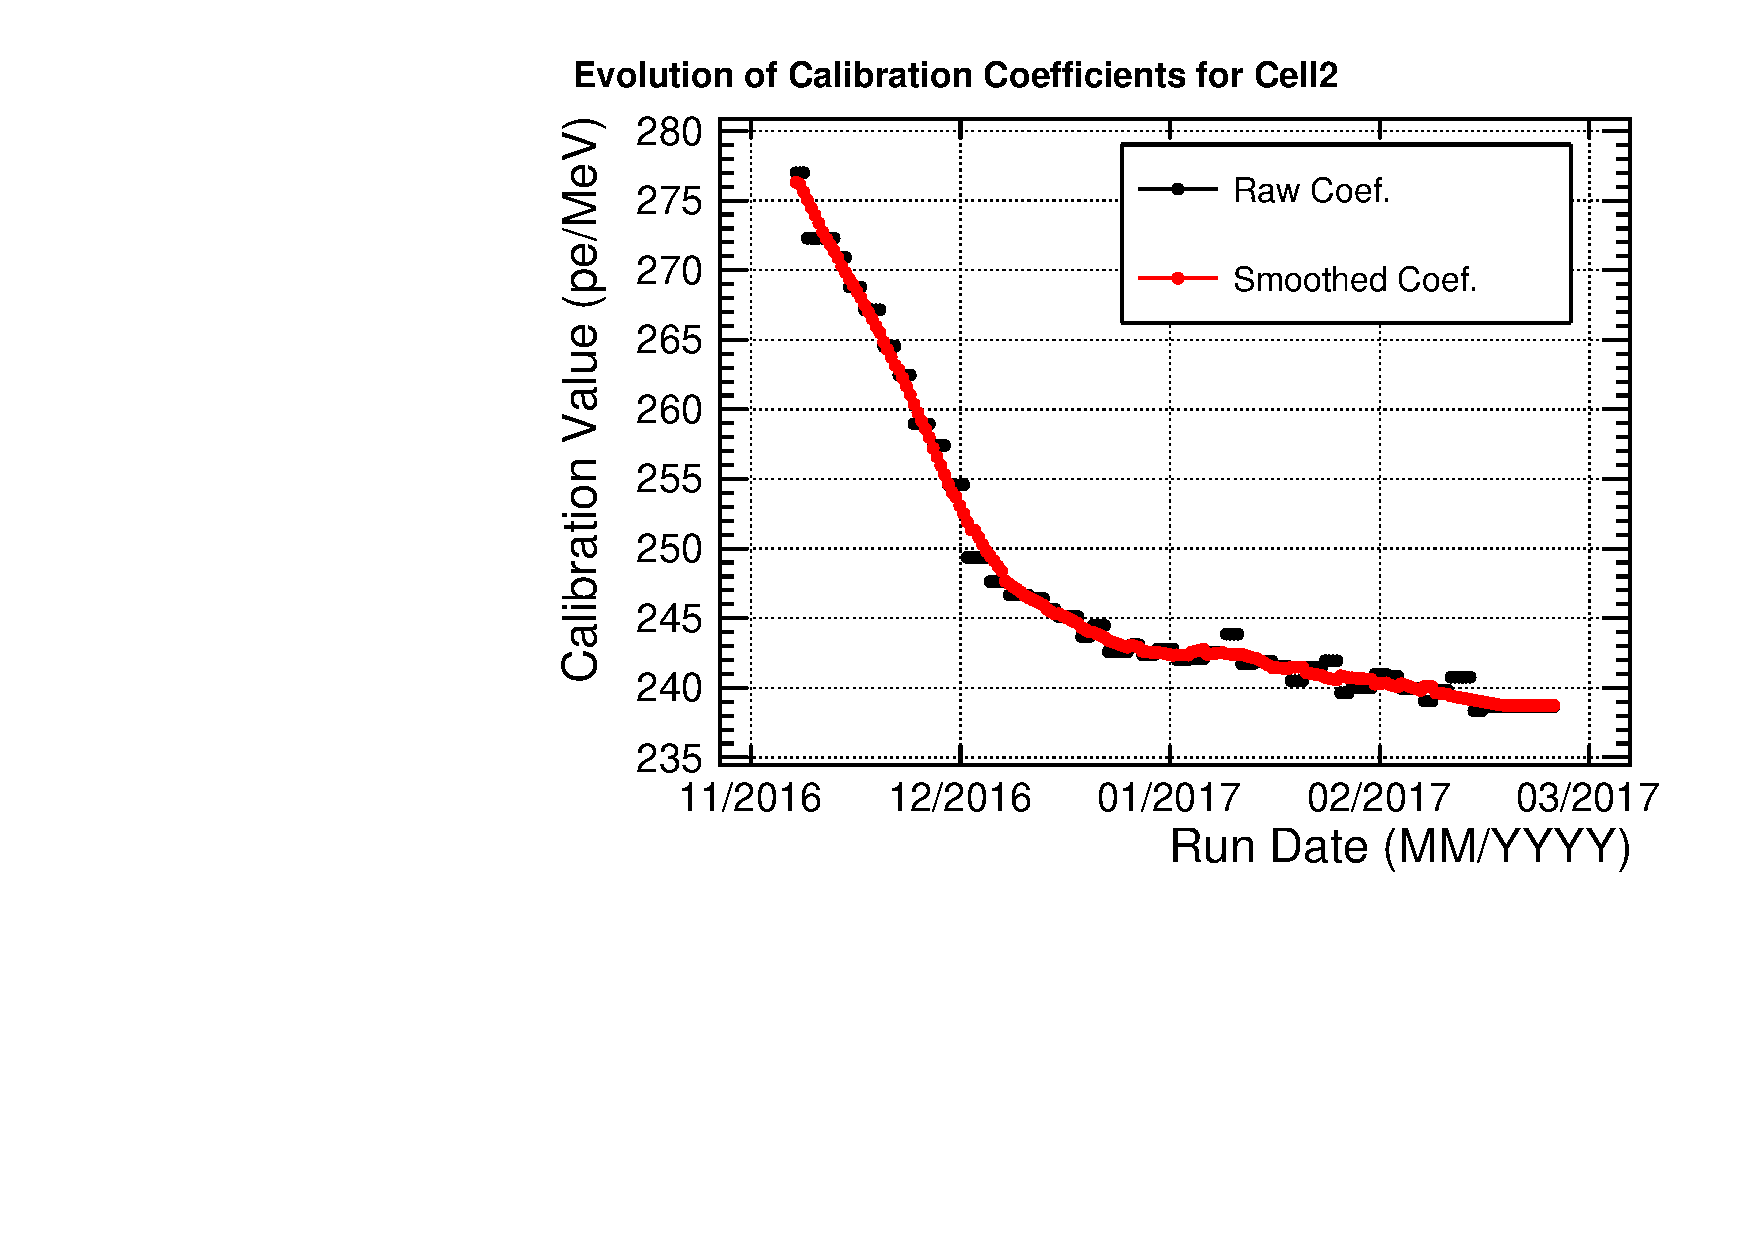
\includegraphics[width=0.85\linewidth]{images/cc_smoothing_show.pdf}
  \caption[Illustration du lissage des coefficients de calibration]{Illustration du lissage des coefficients de calibration. La courbe noire représente la valeur des coefficients brute prise à chaque date, tandis que la courbe rouge montre les coefficients échantillonnés après la procédure de lissage. La période étudiée ici correspond à la phase 1.}
  \label{fig:cc_smoothing_show.pdf}
\end{figure}
\clearpage
}

\afterpage{

\begin{figure}[h!]

\centering

\begin{subfigure}[b]{0.49\textwidth}

\centering
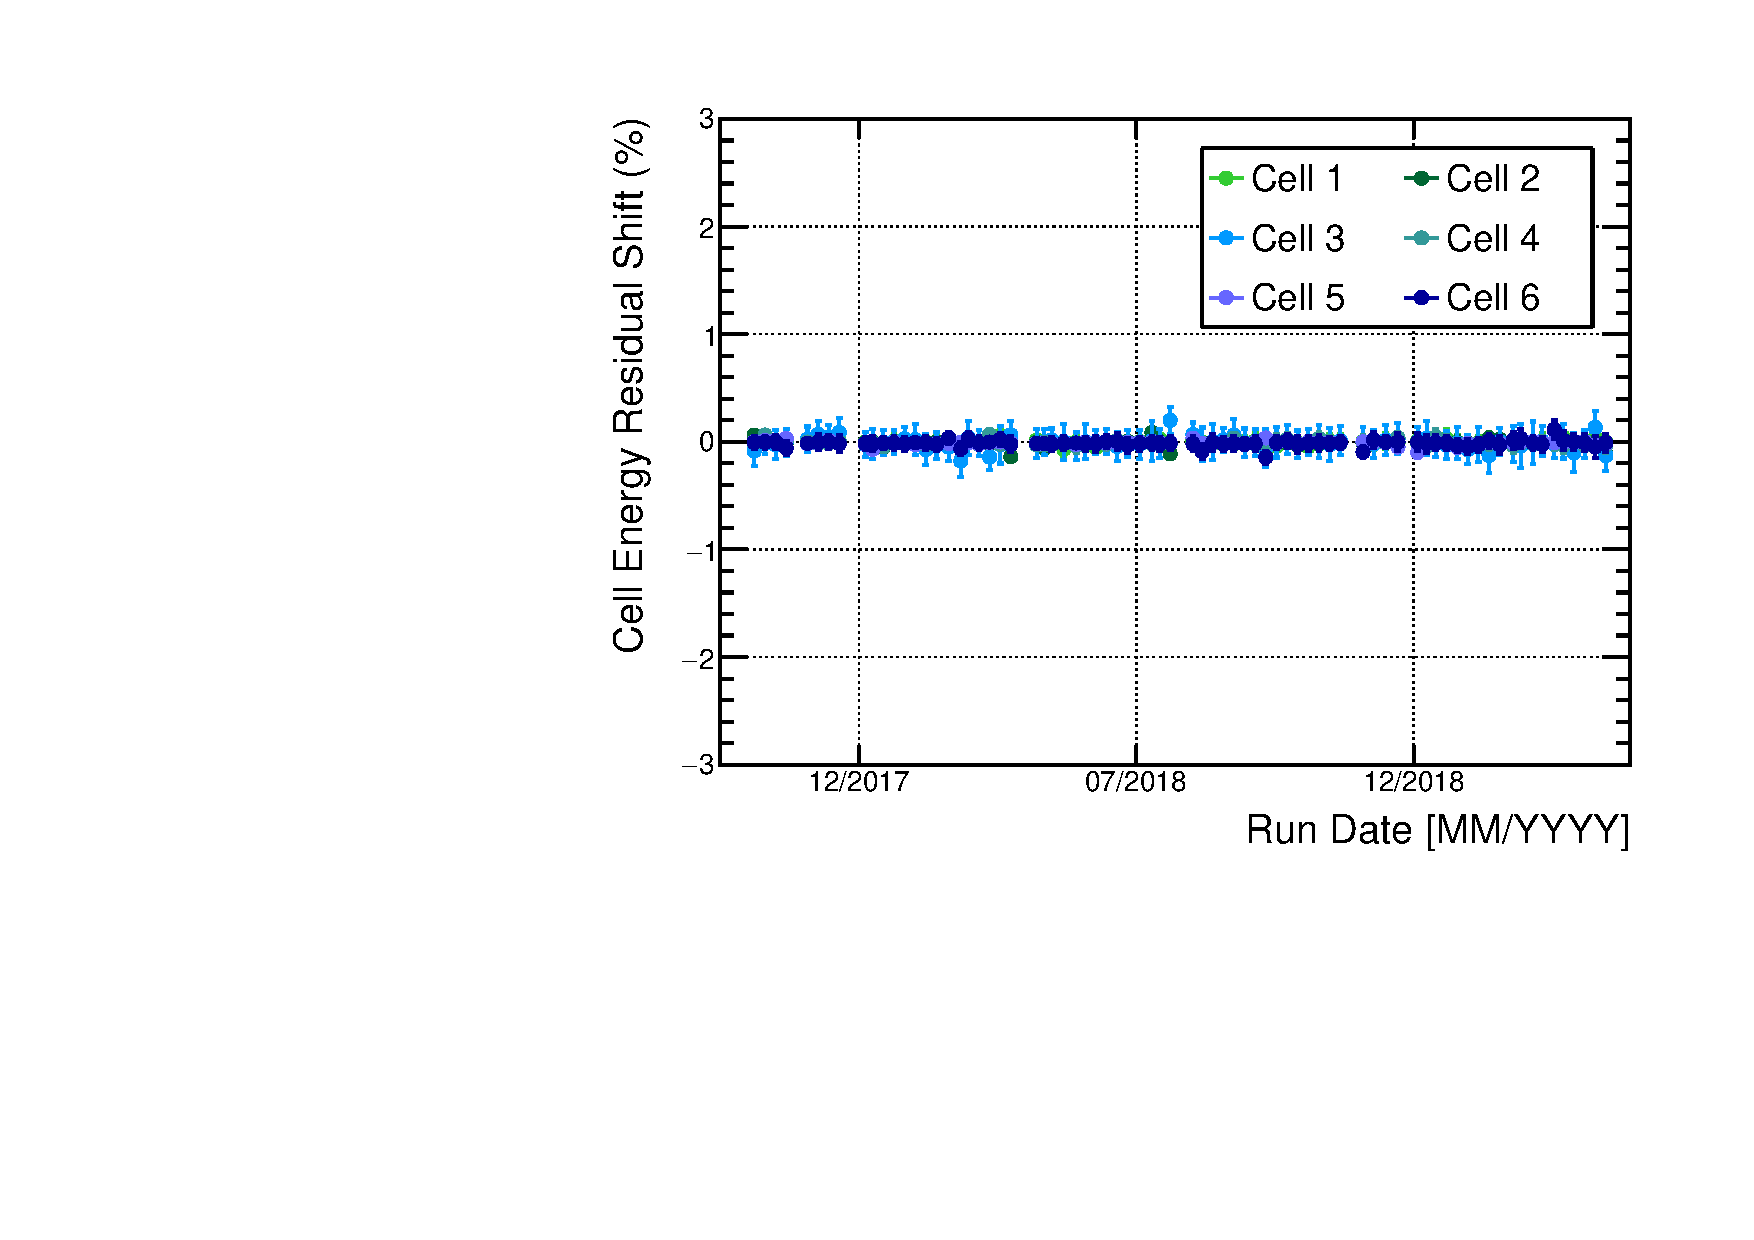
\includegraphics[width=1\textwidth]{images/ErecCell_anchoring_phase-2.pdf}
\caption{$\delta E_{i} / E_{i}$}
\label{fig:ErecCell_anchoring_phase-2.pdf}

\end{subfigure}
~ % attention ! space sensitive
\begin{subfigure}[b]{0.49\textwidth}

\centering
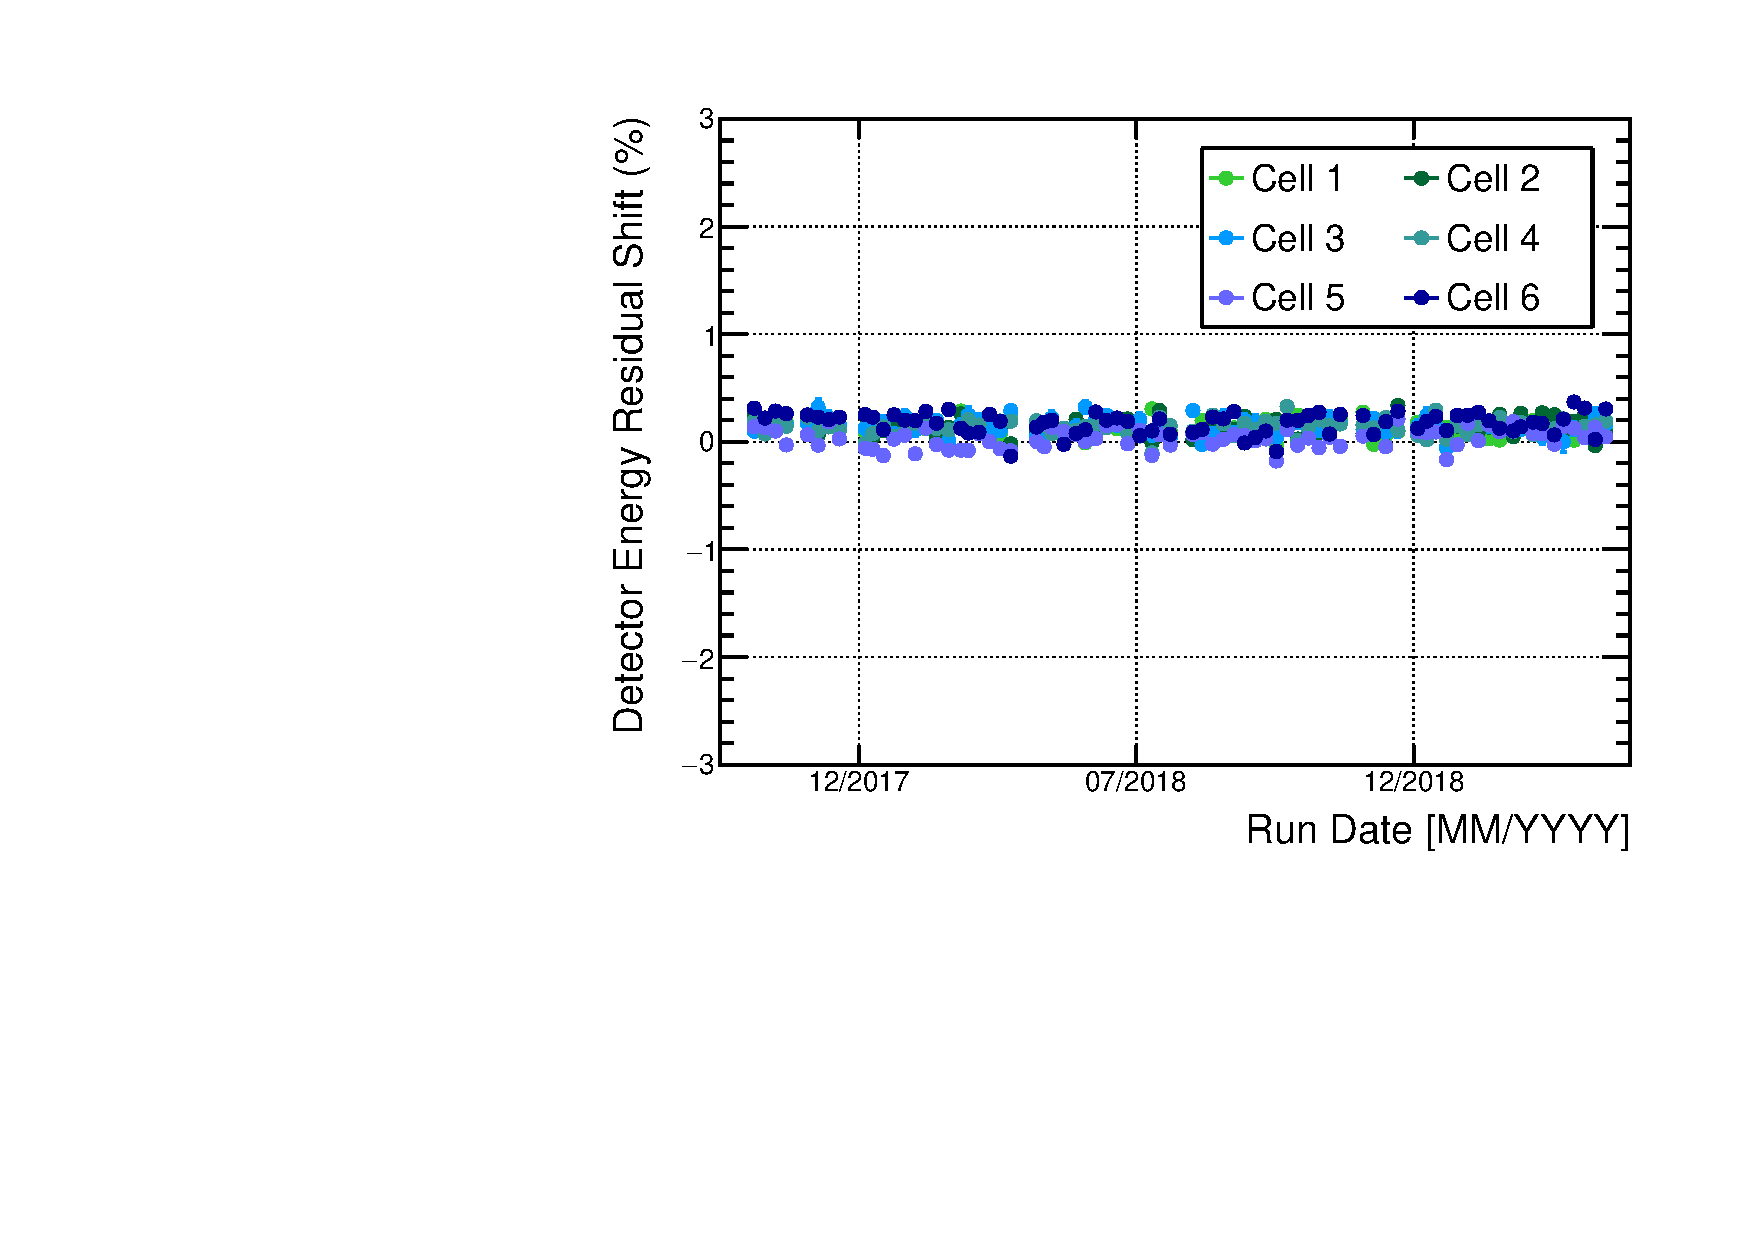
\includegraphics[width=1\textwidth]{images/ErecFull_anchoring_phase-2.pdf}
\caption{$\delta E_{tot} / E_{tot}$}
\label{fig:ErecFull_anchoring_phase-2.pdf}

\end{subfigure}
  \caption[Décalages résiduels de l'énergie reconstruite entre les données et la simulation après ajustement des paramètres de collection de lumière]{Décalages résiduels de l'énergie reconstruite entre les données et la simulation après ajustement des paramètres de collection de lumière. (a) montre les décalages résiduels sur l'énergie reconstruite dans la cellule et (b) montre les décalages résiduels l'énergie reconstruite dans tout le détecteur.}
  \label{fig:Erec_vs_anchor_vs_time}
\end{figure}

\begin{figure}[h!]

\centering

\begin{subfigure}[b]{0.49\textwidth}
\centering
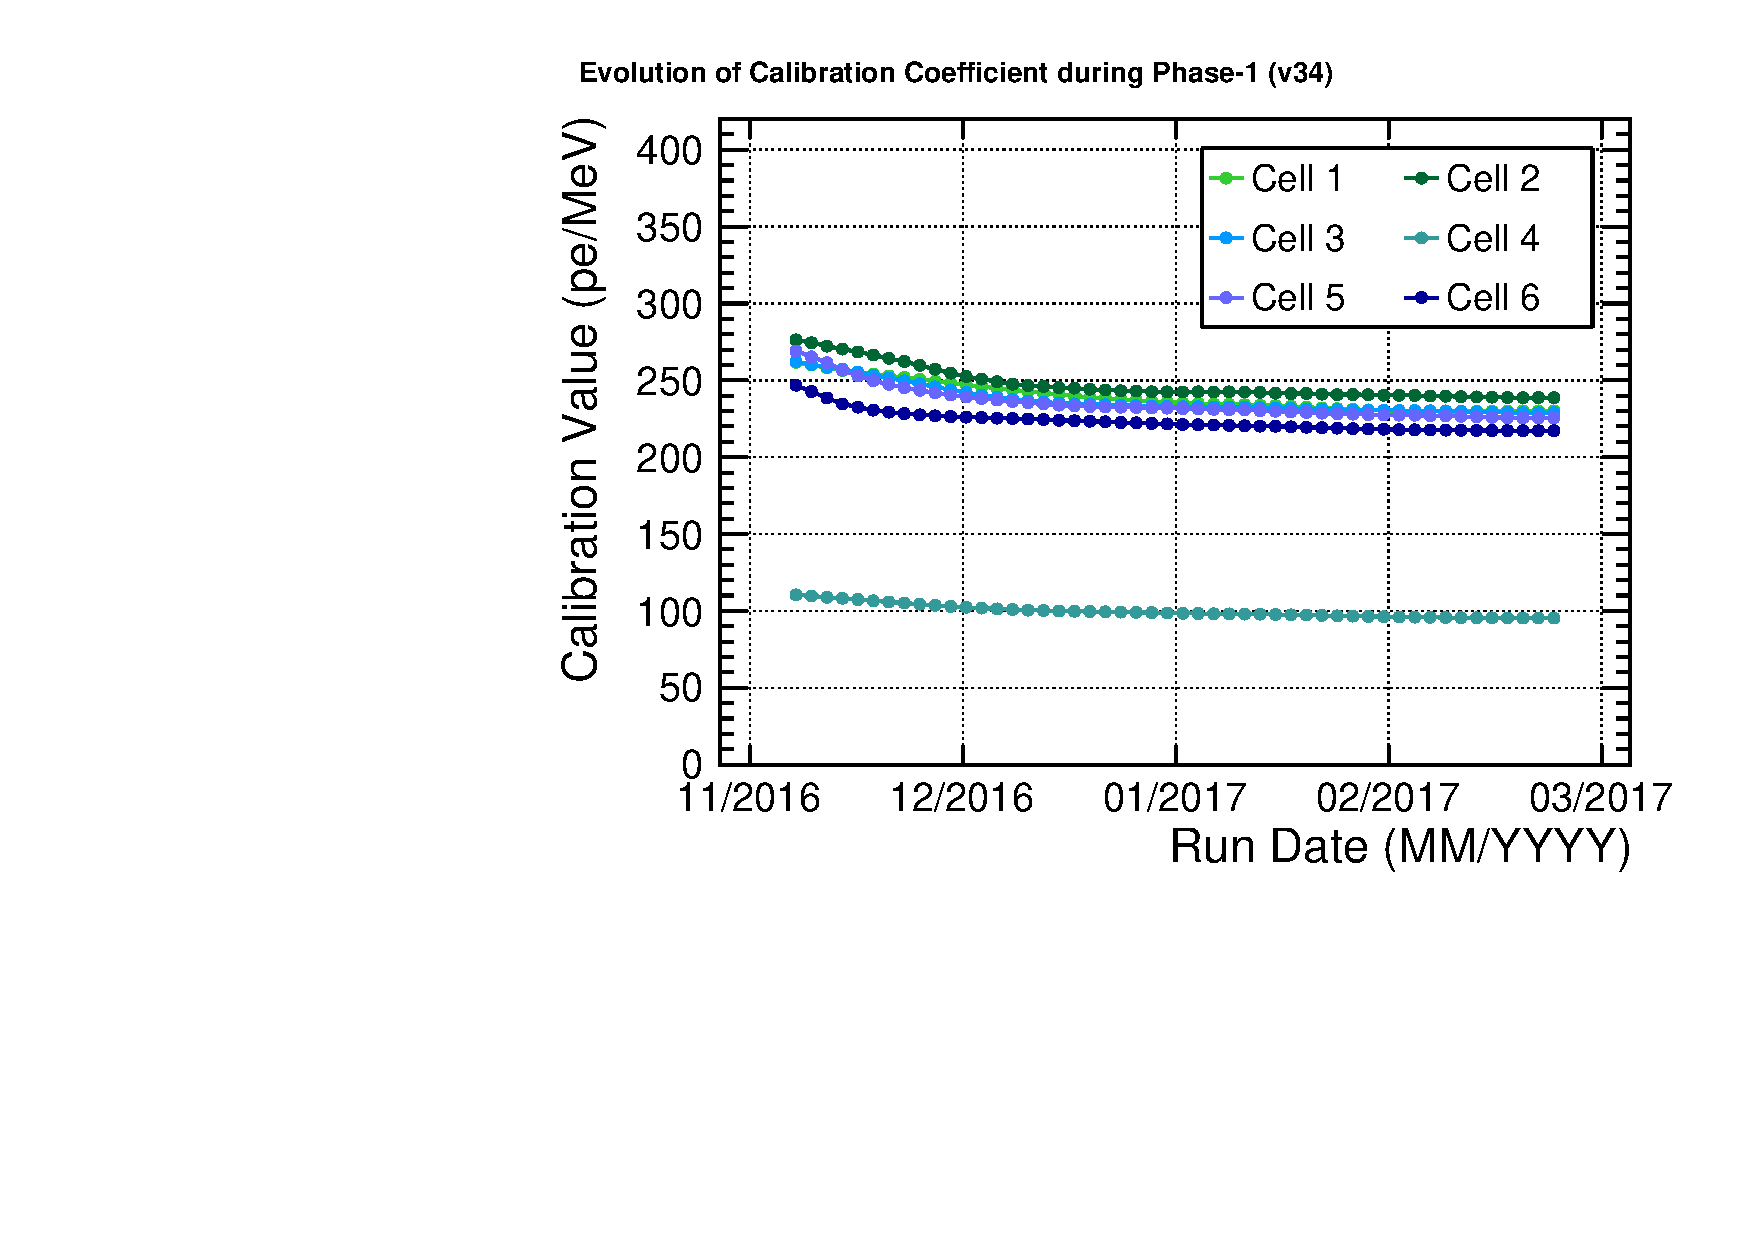
\includegraphics[width=1\textwidth]{images/CC_running_T_p1.pdf}
\caption{Target Cells, phase 1}
\label{fig:CC_running_T_p1.pdf}
\end{subfigure}
~ % attention ! space sensitive
\begin{subfigure}[b]{0.49\textwidth}
\centering
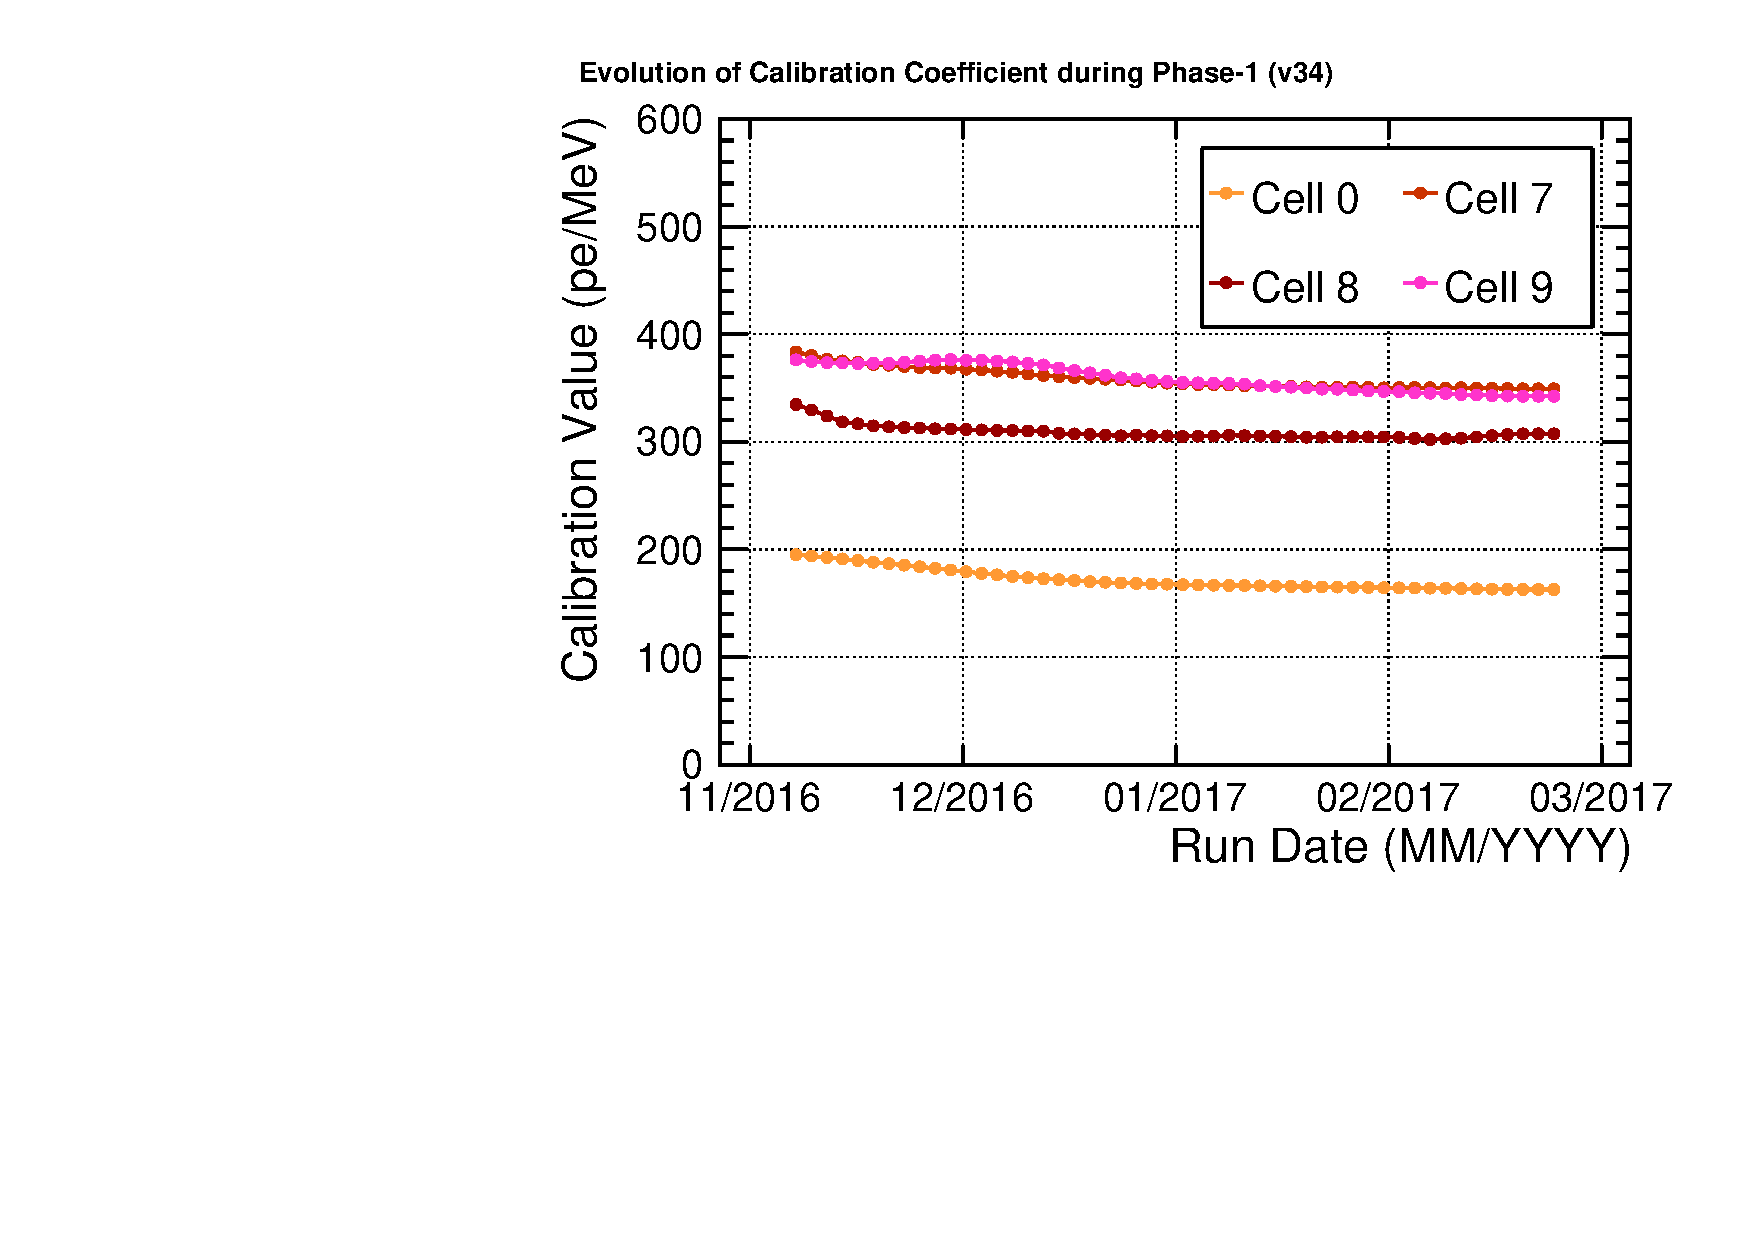
\includegraphics[width=1\textwidth]{images/CC_running_GC_p1.pdf}
\caption{GC Cells, phase 1}
\label{fig:CC_running_GC_p1.pdf}
\end{subfigure}
~ % attention ! space sensitive
\begin{subfigure}[b]{0.49\textwidth}
\centering
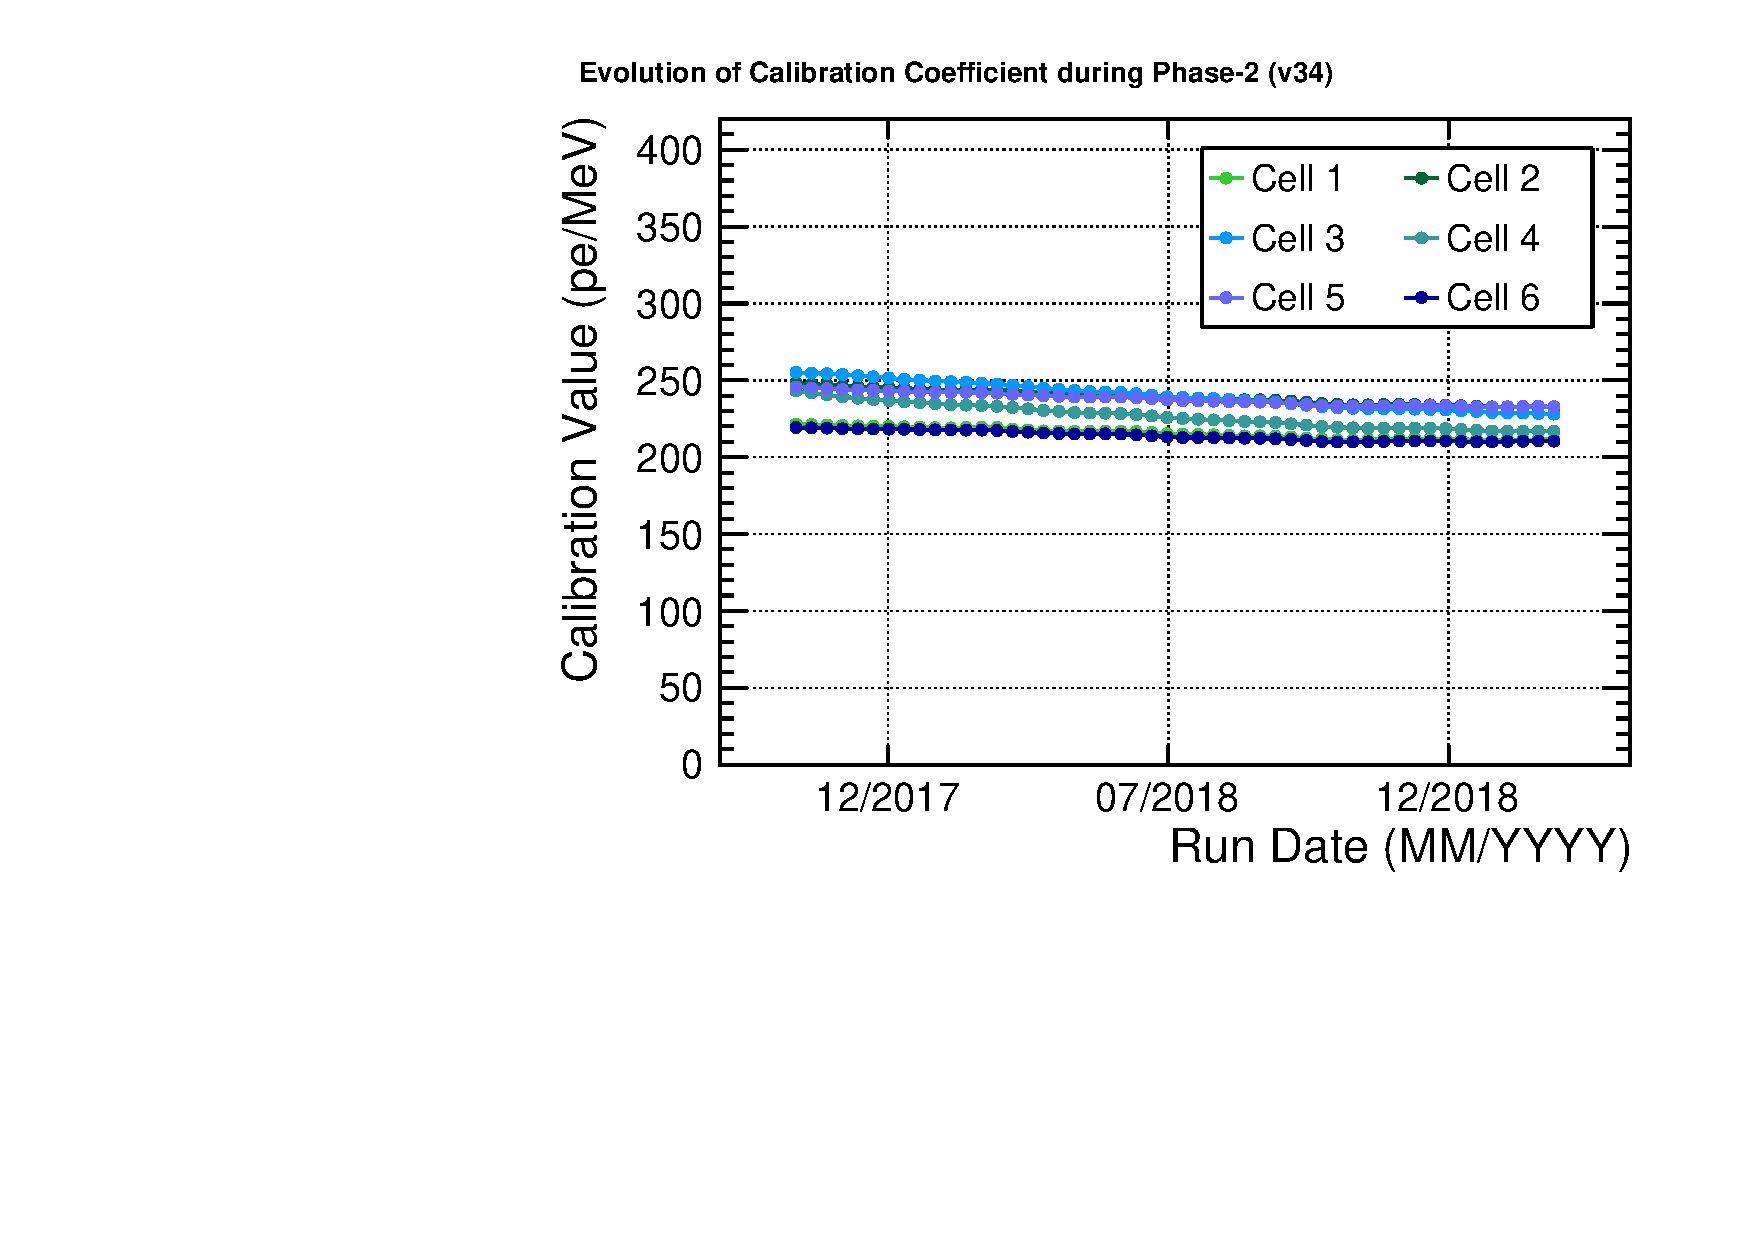
\includegraphics[width=1\textwidth]{images/CC_running_T_p2.pdf}
\caption{Target Cells, phase 2}
\label{fig:CC_running_T_p2.pdf}
\end{subfigure}
~ % attention ! space sensitive
\begin{subfigure}[b]{0.49\textwidth}
\centering
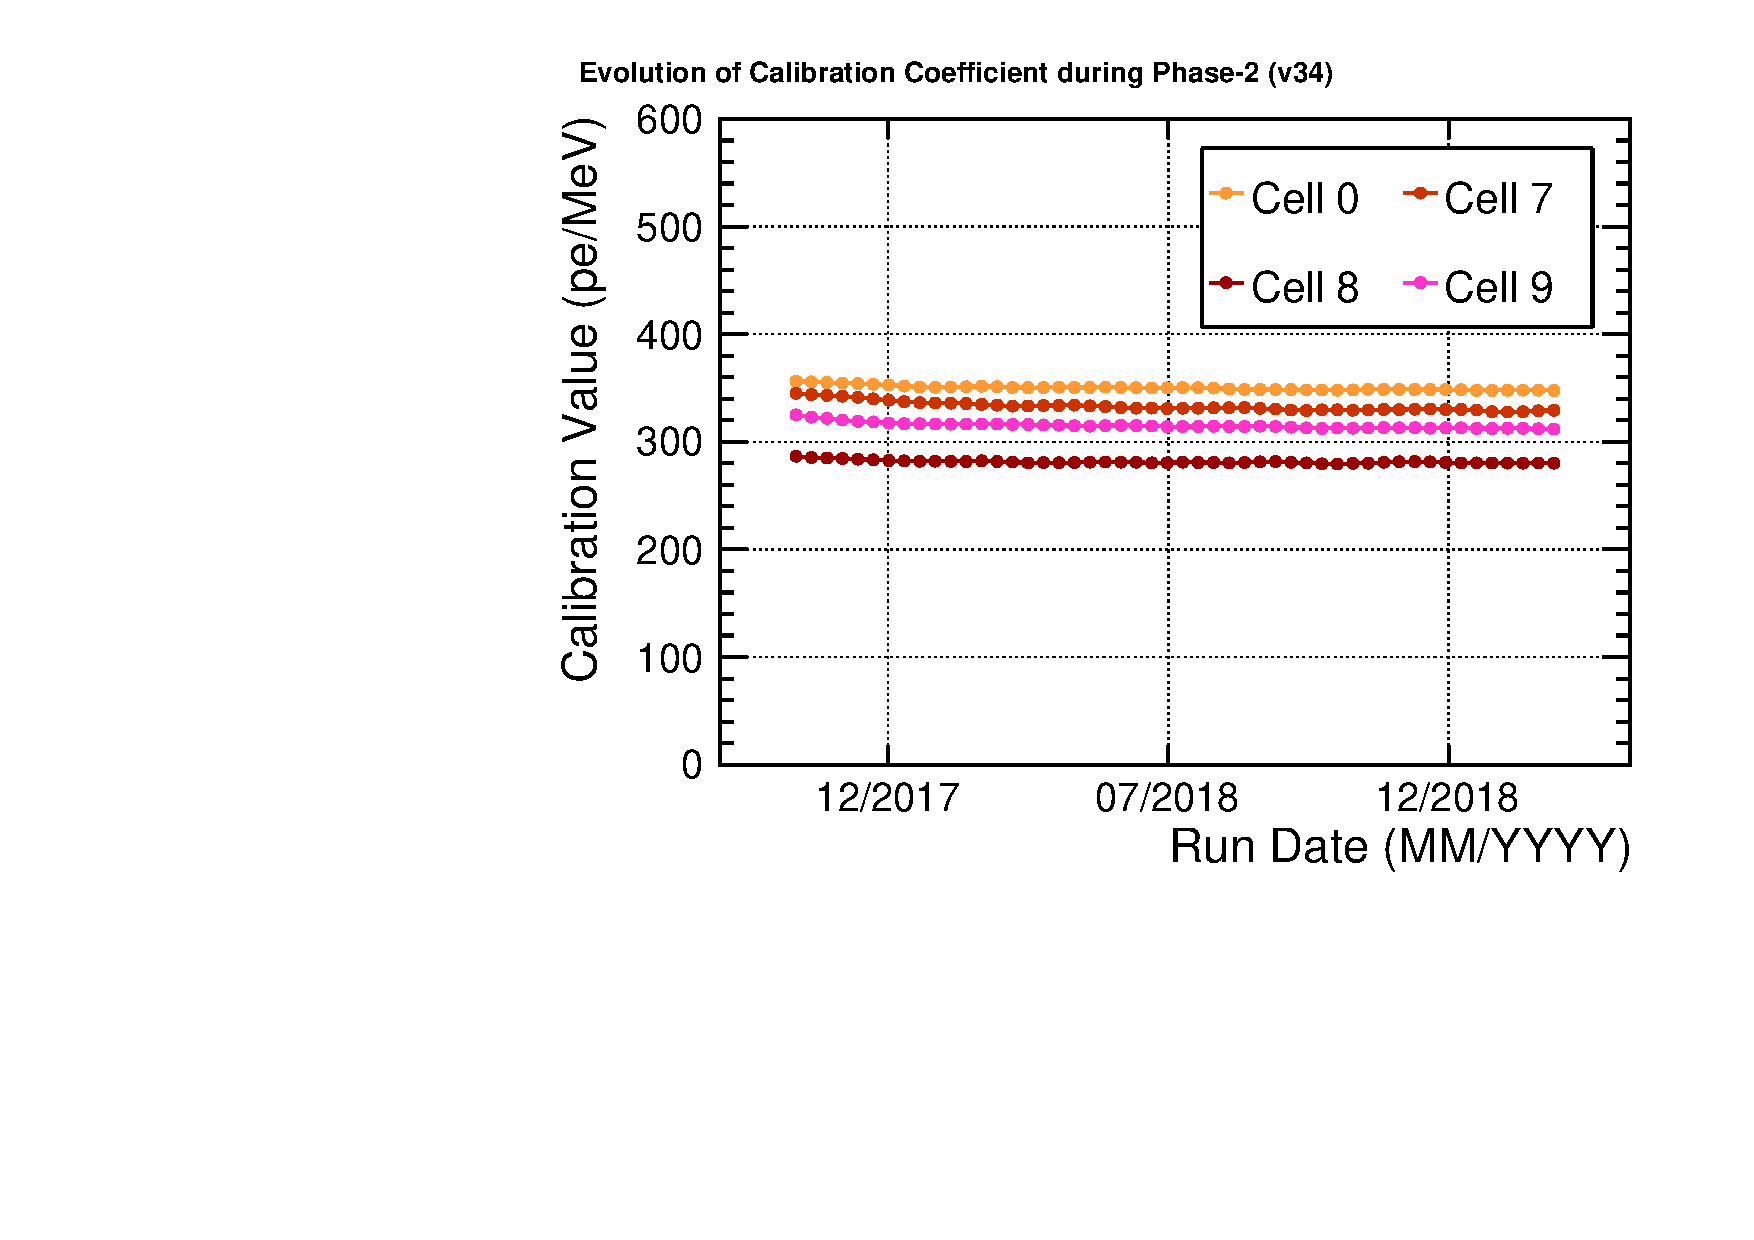
\includegraphics[width=1\textwidth]{images/CC_running_GC_p2.pdf}
\caption{GC Cells, phase 2}
\label{fig:CC_running_GC_p2.pdf}
\end{subfigure}
  \caption[Évolution de la réponse en énergie de chaque cellule pendant la prise de données]{Évolution de la réponse en énergie de chaque cellule pendant la prise de données. (a) et (b) montrent l'évolution des coefficients de calibration pendant la phase 1 des cellules de la Target et du Gamma-Catcher respectivement. Pareillement (c) et (d) montrent l'évolution des coefficients de calibration pendant la phase 2. Les coefficients échantillonnés ont subi l'étape de lissage au préalable.}
  \label{fig:CC_vs_time}
\end{figure}

\clearpage

}

\subsection{Post-traitement}

Au début de la phase 1, les coefficients de calibration ont diminué de près de 15 \% en deux mois. L'écart entre deux dates de calibration était trop important pour être ignoré lors de l'analyse des runs neutrinos. Une interpolation linéaire a donc été mise en place pour prendre en compte l'évolution brutale des $C_i$ et $L_{ij}$. Lorsqu'un run neutrino est analysé, les coefficients de collection de lumière sont échantillonnés sur les 5 dates de calibration les plus proches. Une fonction affine est ajustée sur ces valeurs et les coefficients associés au run neutrino sont obtenus en reportant la date sur la courbe ajustée. Cette étape de post-traitement à eu pour effet de lisser l'évolution des $C_i$ et $L_{ij}$ utilisés dans l'analyse des données. L'effet est présenté sur la figure \ref{fig:cc_smoothing_show.pdf}.

\bigbreak


\subsection{Conclusions sur l'ancrage}
\label{sec:cc_encrage}

La procédure d'ajustement des paramètres de collection de lumière a été appliquée sur l'ensemble des données des sessions de calibration $\ce{^{54}Mn}$ en phases 1 et 2. Aujourd'hui, l'ancrage est effectué automatiquement toutes les semaines dès qu'une nouvelle calibration $\ce{^{54}Mn}$ a lieu. Le suivi de chaque valeur de $C_i$ et $L_{ij}$ est affiché sur le site du monitoring et permet d'analyser le comportement de la réponse du détecteur en temps réel. À titre d'illustration, l'évolution des $C_i$ est présenté pour les deux phases sur la figure \ref{fig:CC_vs_time}.\\

En phase 1, les deux cellules qui ont perdu leur couplage optique à cause d'une fuite des \textit{buffers} sont la 0 (GC-Front) et la 4. Elles se distinguent des autres par un coefficient de calibration anormalement faible. En effet la cellule 4 ne récoltait que $\sim \SI{100}{pe/MeV}$ soit plus de deux fois moins que les autres cellules de la Target. Il en va de même avec la cellule 0 qui ne voit que $\sim \SI{175}{pe/MeV}$ alors que 350 serait attendu. On remarque aussi une tendance décroissante corrélée entre les cellules de la Target jusque fin décembre 2016. Cette évolution a été attribuée à la dégradation progressive des parois réfléchissantes lorsque le liquide scintillateur a pénétré le sandwich en acrylique. En effet, la corrélation avec le développement des coefficients de fuites de lumière $L_{ij}$ s'est montrée en faveur de cette hypothèse. Contrairement à ce que cette diminution des $C_i$ laisse penser, le rendement lumineux du liquide ($LY_i$) n'a pas montré d'évolution significative pendant ces périodes. Si tel était le cas, le nombre total de charges collectées par MeV devrait suivre la même tendance:

\begin{equation}
    Q^\textrm{total}(E_i = \SI{1}{MeV}, E_{j \neq i} = 0) = \sum_j Q_j = \sum_j C_iL_{ij} = \sum_j M_{ij}.
\end{equation}

\afterpage{

\begin{figure}[h!]

\centering

\begin{subfigure}[b]{0.49\textwidth}
\centering
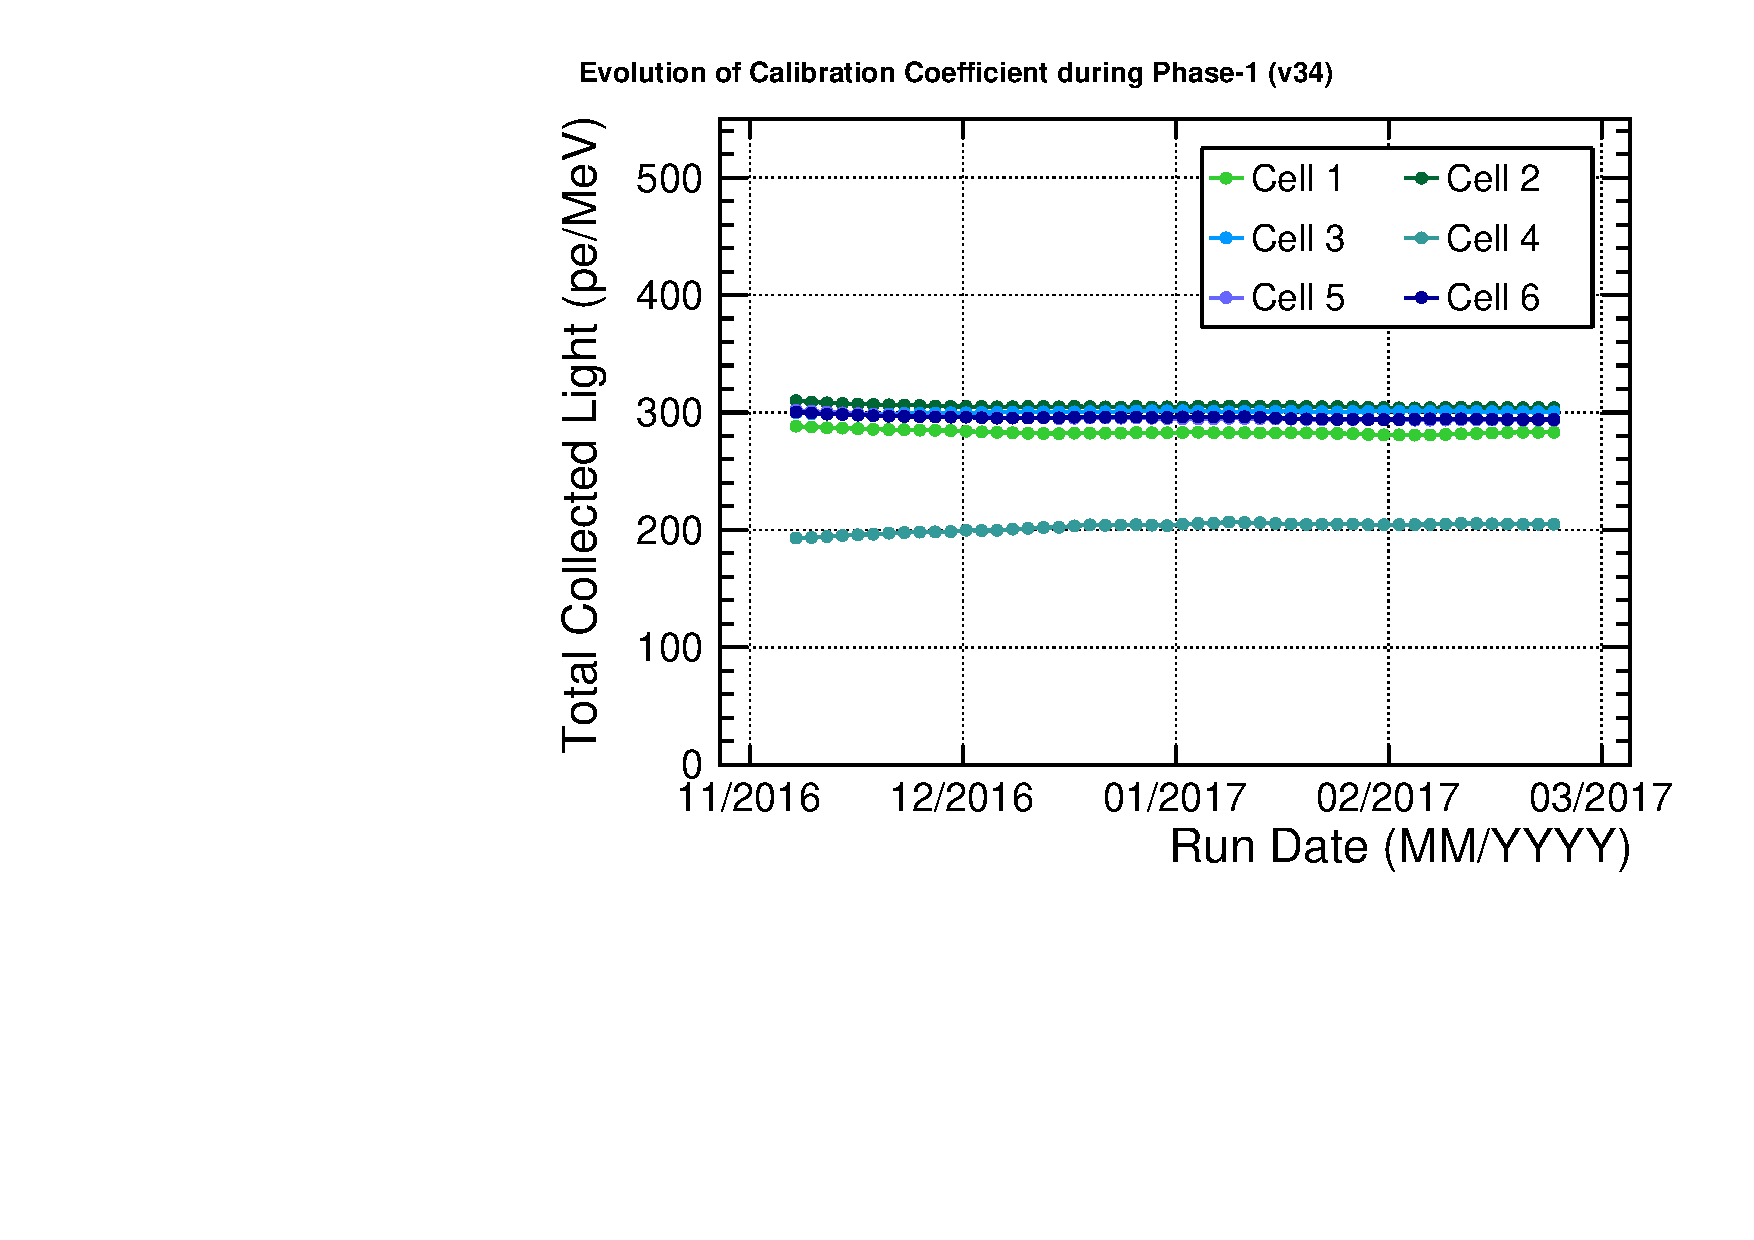
\includegraphics[width=1\textwidth]{images/LY_running_T_p1.pdf}
\caption{Target Cells, phase 1}
\label{fig:LY_running_T_p1.pdf}
\end{subfigure}
~ % attention ! space sensitive
\begin{subfigure}[b]{0.49\textwidth}
\centering
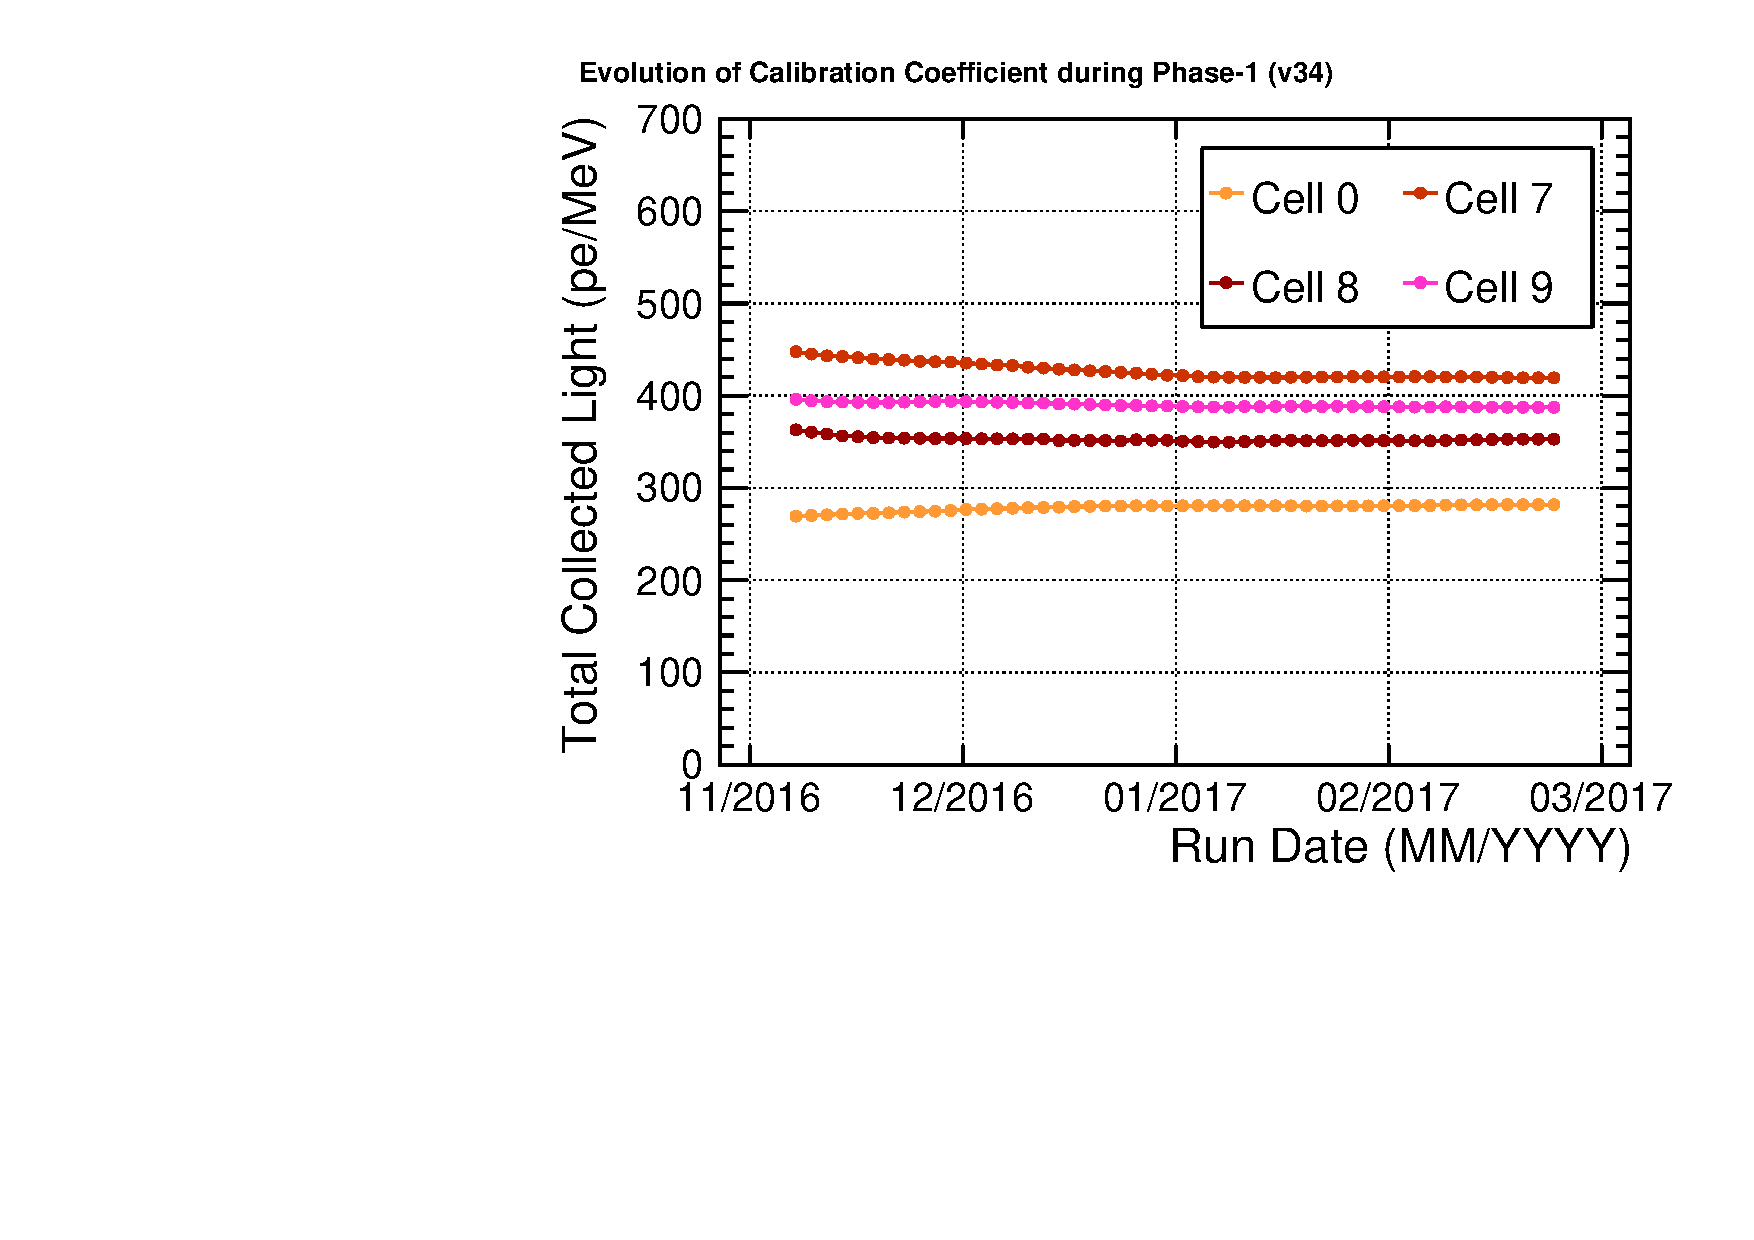
\includegraphics[width=1\textwidth]{images/LY_running_GC_p1.pdf}
\caption{GC Cells, phase 1}
\label{fig:LY_running_GC_p1.pdf}
\end{subfigure}
~ % attention ! space sensitive
\begin{subfigure}[b]{0.49\textwidth}
\centering
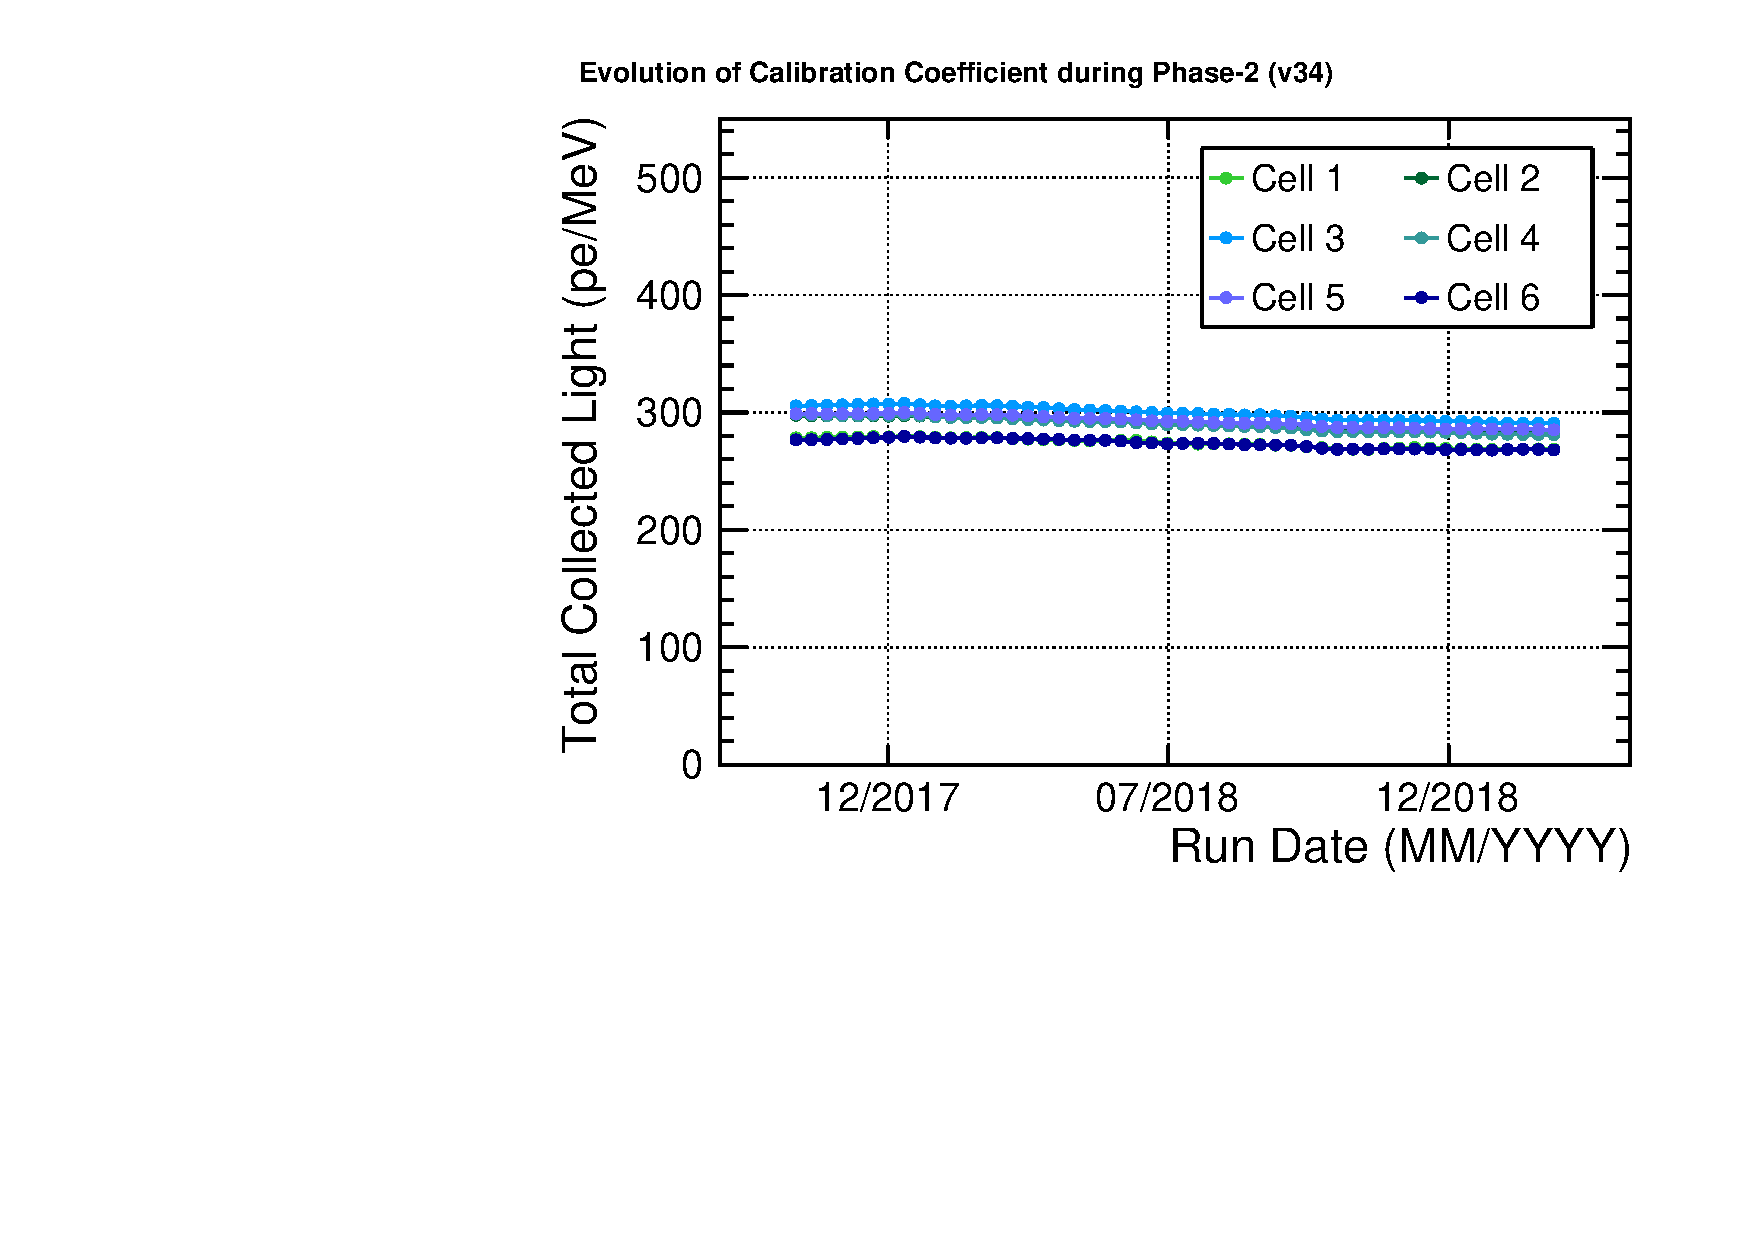
\includegraphics[width=1\textwidth]{images/LY_running_T_p2.pdf}
\caption{Target Cells, phase 2}
\label{fig:LY_running_T_p2.pdf}
\end{subfigure}
~ % attention ! space sensitive
\begin{subfigure}[b]{0.49\textwidth}
\centering
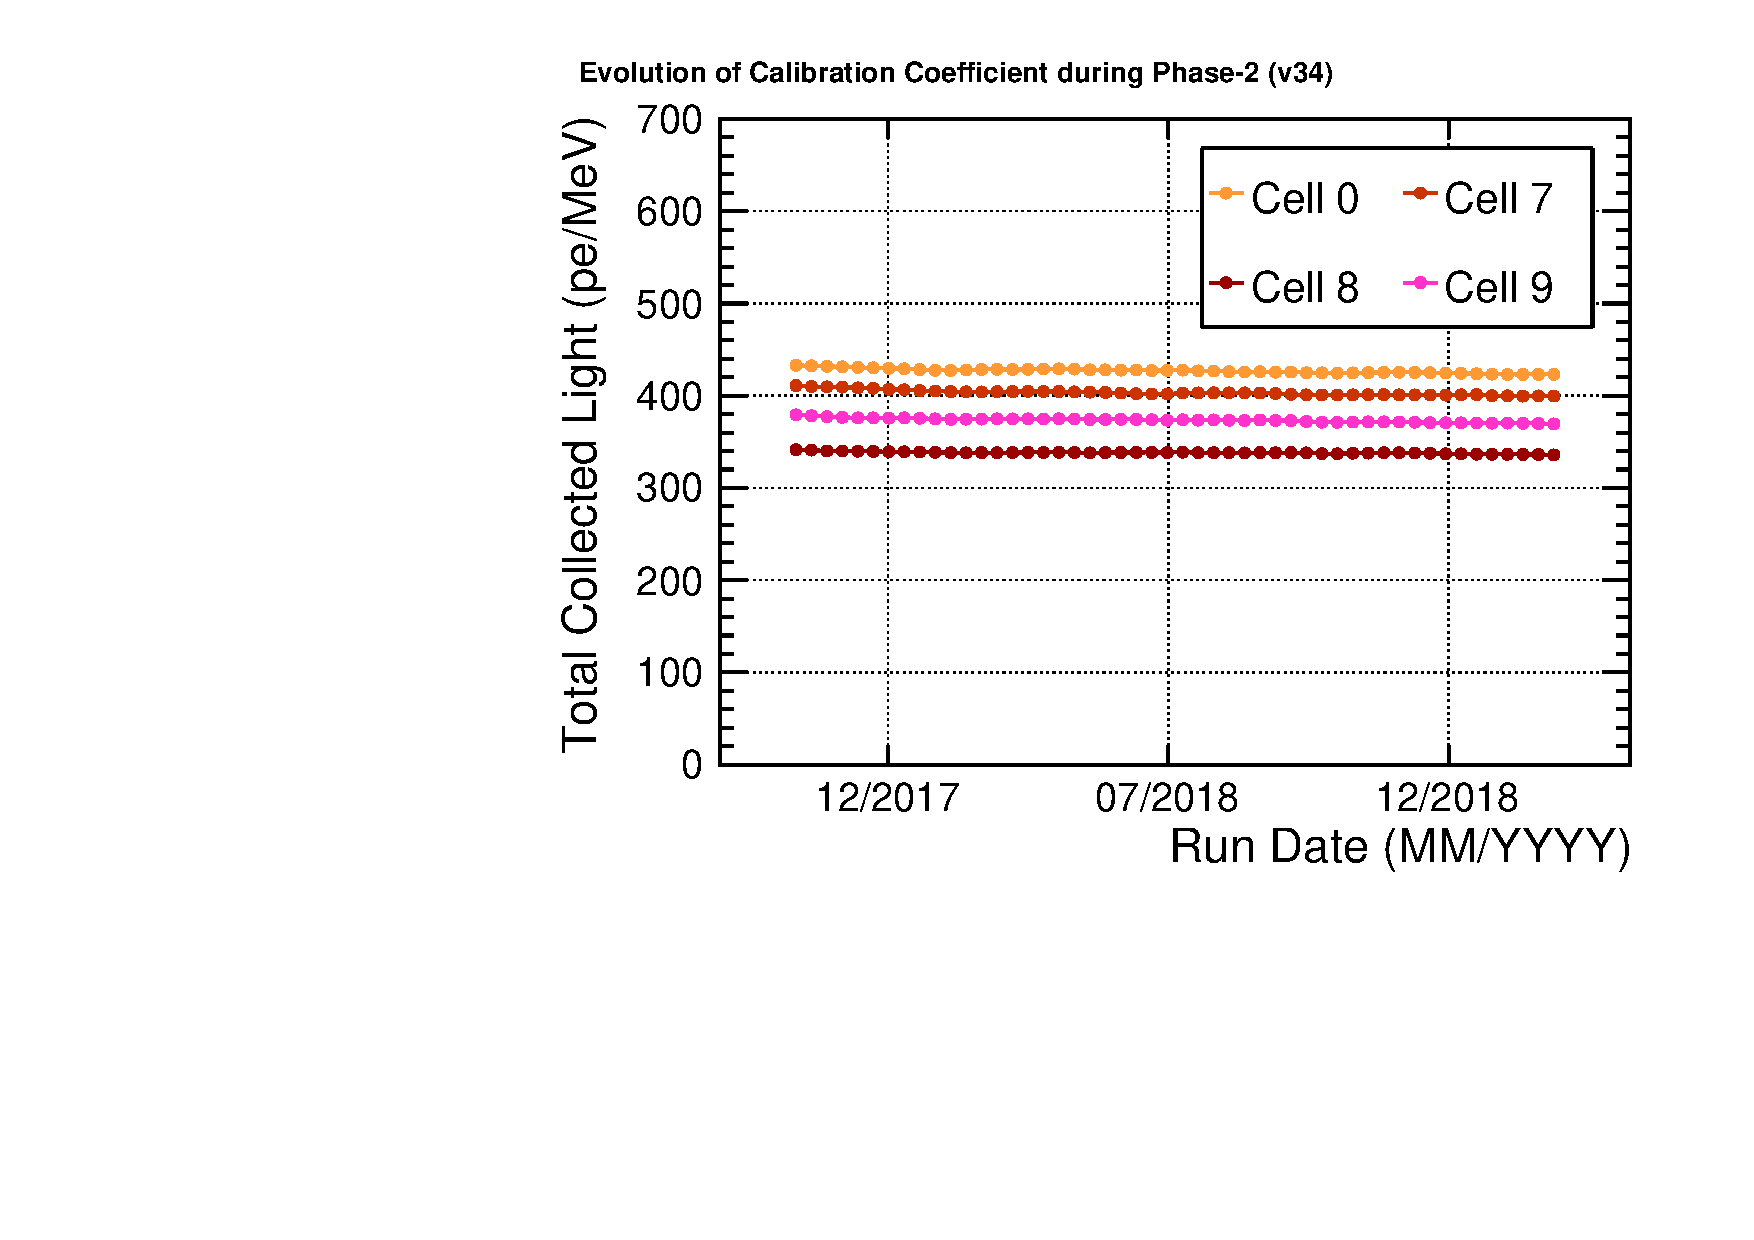
\includegraphics[width=1\textwidth]{images/LY_running_GC_p2.pdf}
\caption{GC Cells, phase 2}
\label{fig:LY_running_GC_p2.pdf}
\end{subfigure}
  \caption[Évolution de l'efficacité de collection de lumière totale  pendant la prise de données]{Évolution de l'efficacité de collection de lumière totale  pendant la prise de données]. (a) et (b) montrent l'évolution de $Q^\textrm{total} = \sum_j M_{ij}$ pendant la phase 1 des cellules de la Target et du Gamma-Catcher respectivement. Pareillement (c) et (d) montrent l'évolution de $Q^\textrm{total}$ pendant la phase 2.}
  \label{fig:LY_vs_time}
\end{figure}

}

Or comme le montre la figure \ref{fig:LY_vs_time}, cette quantité ne diminue pas. La baisse des $C_i$ s'explique par le fait que les photons perdus dans la cellule $i$ sont en fait collectés par les cellules voisines $j$. On remarque d'ailleurs que contrairement aux autres, la cellule 4 voit $Q^\textrm{total}$ augmenter. Cette accroissement du nombre de photons total collectés est du au développement des fuites de lumière, car l'efficacité de collection de la cellule 4 ($\alpha_i$) est faible donc la lumière émise dans 4 est préférentiellement collectée dans les cellules voisines via les fuites de lumière. En plus de démontrer une stabilité satisfaisante de l'efficacité de collection totale du détecteur, la figure \ref{fig:LY_vs_time} affirme la stabilité du rendement lumineux du liquide pendant toute la phase 1.\\

Après réparation des buffers défaillants et amélioration de l'étanchéité des sandwichs en acrylique, la phase 2 offre une grande stabilité des coefficients de calibration de la Target et du Gamma-Catcher comme le montre la figure \ref{fig:CC_vs_time}. Sur un an cependant, les $C_i$ de la Target montrent une tendance décroissante sensible ($\sim \SI{-10}{\% / an}$). Par ailleurs, l'efficacité totale de collection de la Target diminue elle aussi, bien que l'amplitude de la chute soit plus faible: $\sim \SI{-5}{\% / an}$ (figure \ref{fig:LY_vs_time}). L'évolution des $C_i$ semble donc être principalement dû au lent développement des fuites de lumière pendant la phase 2, tandis que la baisse résiduelle du nombre total de photons collectés pourrait indiquer une légère dégradation des propriétés optiques du liquide scintillateur de la Target. Du reste, aucune évolution résiduelle sur $Q^\textrm{total}$ pour les cellules du Gamma-Catcher ne peut être affirmée.\\

\bigbreak

\section{Ajustement des paramètres de la simulation}

Comme nous l'avons explicité dans la Section \ref{seq:Erec_formalisme}, la procédure de reconstruction en énergie ne corrige les inhomogénéités de collection de lumière qu'au premier ordre. De plus, les effets de non-linéarité du processus de scintillation ne sont pas pris en compte. Les paramètres de la simulation doivent être ajustés et contrôlés pour assurer la réponse à plus haute énergie.\\

Pour ce faire, d'autres sources gamma à différentes énergies ont été déployées. Les gammas de haute énergie permettent non seulement de mesurer l'évolution du rendement lumineux, mais aussi de tester les effets de volume. Effectivement, la distance moyenne sans interaction d'un gamma augmente avec l'énergie : environ $\SI{20}{cm}$ à $\SI{1}{MeV}$ contre $\SI{30}{cm}$ à $\SI{2}{MeV}$. Les différentes sources radioactives utilisées sont listées dans le Tableau \ref{tab:quencing_sources}.\\

\afterpage{
\begin{table}
  \centering
    \begin{tabular}{|l|c|c|}
      \hline
      \textbf{Source} & \textbf{Energie (MeV)} & \textbf{Multiplicité}\\
      \hline
      $\ce{^{68}Ge}$ & 0.5110 & 2\\
      \hline
      \multirow{2}{*}{$\ce{^{124}Sb}$} & 0.6027 & \multirow{2}{*}{2}\\
      & 1.691 &\\
      \hline
      $\ce{^{137}Cs}$ & 0.6617 & 1\\
      \hline
      $\ce{^{54}Mn}$ & 0.8348 & 1\\
      \hline
      $\ce{^{65}Zn}$ & 1.116 & 1\\
      \hline
      \multirow{2}{*}{$\ce{^{60}Co}$} & 1.173 & \multirow{2}{*}{2}\\
      & 1.332 &\\
      \hline
      $\ce{^{42}K}$ & 1.525 & 1\\
      \hline
      \multirow{2}{*}{$\ce{^{24}Na}$} & 1.369 & \multirow{2}{*}{2}\\
      & 2.754 & \\
      \hline
      \multirow{2}{*}{$\ce{AmBe}$} & 4.440 & 1 + neutron\\
      & 2.223 (n-H) & 1\\
      \hline
    \end{tabular}
    \caption[Liste des sources gamma utilisées pour la calibration]{Liste des sources gamma utilisées pour la calibration. La multiplicité désigne le nombre de gammas émis simultanément.}
    \label{tab:quencing_sources}
\end{table}
}



\subsection{Modèle de quenching}

La réponse du détecteur est calibrée avec des gammas de $\SI{0.835}{MeV}$, mais ce sont les électrons produits par effet Compton qui induisent le processus de scintillation. Au fur et à mesure qu'ils ralentissent, leur pouvoir d'arrêt augmente très fortement  et une partie non négligeable de leur énergie initiale est déposée dans une zone très localisée. Le pouvoir de scintillation des molécules du liquide est alors saturé et une partie de l'énergie déposée n'est pas convertie en lumière : c'est l'effet de quenching. Le quenching se manifeste donc par une non-linéarité des coefficients de calibration à basse énergie. Celle-ci doit être contrôlée afin d'assurer la validité de l'échelle en énergie des spectres neutrino. Le quenching est reproduit dans la simulation grâce au modèle effectif de Birks \cite{Birks:1951boa}:

\begin{equation}
    \frac{dL}{dx} = L_0 \frac{\frac{dE}{dx}}{1 + k_B\frac{dE}{dx}},
\end{equation}

\bigbreak

où $dL/dx$ est le rendement lumineux par unité de longueur, $L_0$ le rendement lumineux en régime linéaire, $dE/dx$ le pouvoir d'arrêt de la particule ionisante et $k_B$ une constante appelée \og paramètre de Birks \fg{} dont la valeur dépend du matériau scintillateur. Notons que chaque particule ionisante possède à une énergie donnée, un pouvoir d'arrêt qui lui est propre. Les paramètres de la loi de Birks ($L_0$ et $k_B$) sont donc différents pour chaque particule. Plusieurs méthodes ont été abordées afin d'ajuster le paramètre de Birks. La méthode détaillée ici est celle qui a été développée dans cette thèse : \og Mesure de la divergence Données-Simulations de l'énergie reconstruite\fg{} \cite{docdb468}.\\

Chaque énergie de gamma peut être associée à un quenching électron effectif. En effet, les gammas interagissent soit par effet photoélectrique, soit par diffusion Compton ou encore par création de paires électron-positron. Ces trois interactions se résument à la production de plusieurs électrons à diverses énergies où chacun suit la loi de Birks avec les mêmes paramètres $L_0$ et $k_B$. La réponse en énergie des gammas correspond donc à un quenching électron moyenné :

\begin{equation}
    L(\gamma) = \left<\sum_{e^-} \int_x \frac{dL(e^-)}{dx}dx \right>.
\end{equation}

\afterpage{

\begin{figure}[h!]
\centering

\begin{subfigure}[b]{0.49\textwidth}
\centering
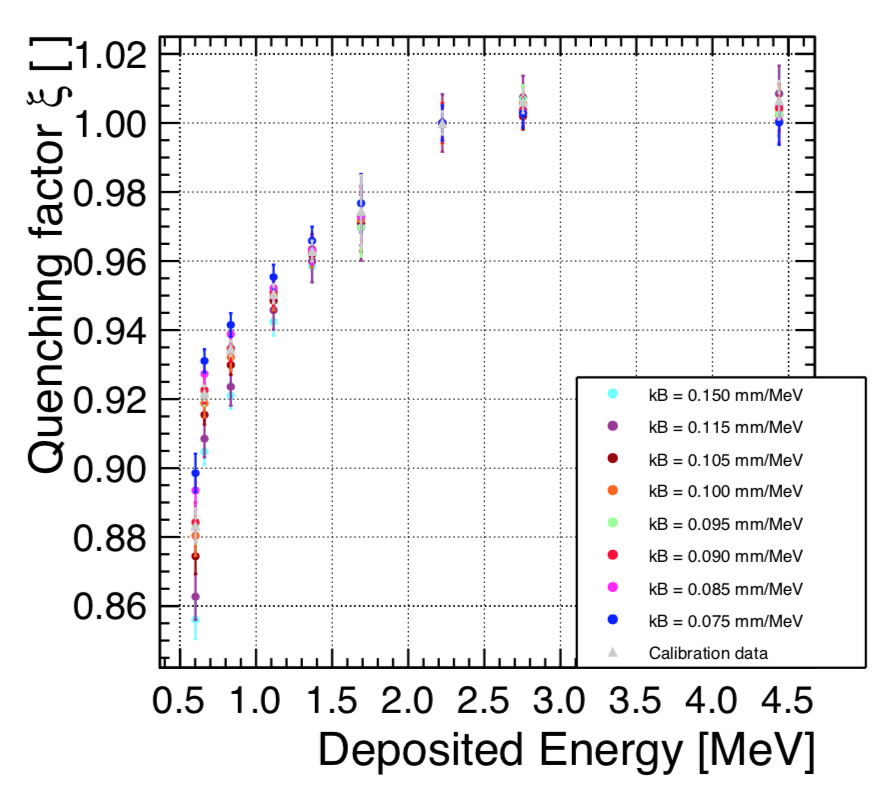
\includegraphics[width=1\textwidth]{images/quenching_vs_E.png}
\caption{}
\label{fig:quenching_vs_E.png}
\end{subfigure}
~ % attention ! space sensitive
\begin{subfigure}[b]{0.49\textwidth}
\centering
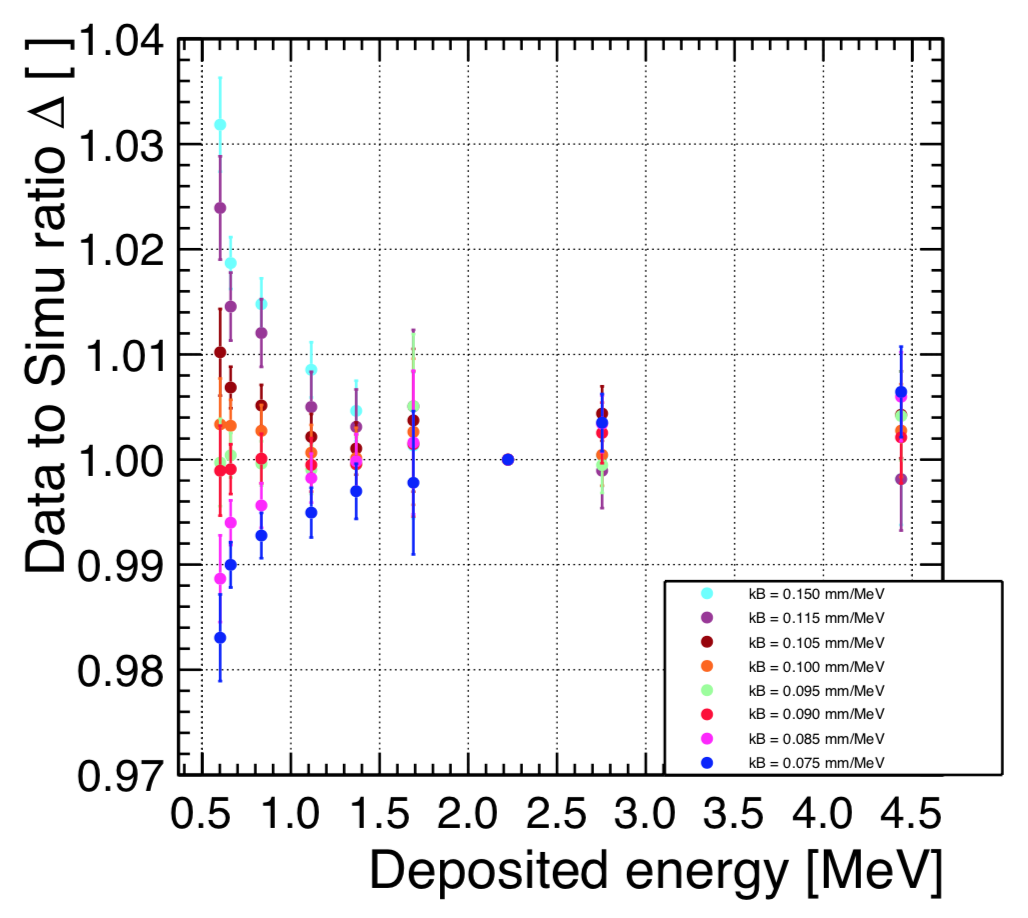
\includegraphics[width=1\textwidth]{images/quenching_ratio_vs_E.png}
\caption{}
\label{fig:quenching_ratio_vs_E.png}
\end{subfigure}

\caption[Illustration de l'effet du quenching sur la simulation]{Illustration de l'effet du quenching sur la simulation. (a) montre l'évolution de la valeur des coefficients de calibration normalisés avec la valeur du pic gamma n-H à $\SI{2.2}{MeV}$ : $\xi \doteq C_i(E) / C_i(\SI{2.2}{MeV})$. (b) représente le rapport $\Delta \doteq \xi(\textrm{Data})/\xi(\textrm{MC})$. Les sources gamma utilisées sont (de gauche à droite): $\ce{^{124}Sb}$, $\ce{^{137}Cs}$, $\ce{^{54}Mn}$, $\ce{^{65}Zn}$, $\ce{^{24}Na}$, $\ce{^{124}Sb}$, $\ce{n-H}$, $\ce{^{24}Na}$, $\ce{AmBe}$. (source \cite{docdb929})}
\label{fig:quenching_effect_on_calib}

\end{figure}

\begin{figure}[h!]
  \centering
  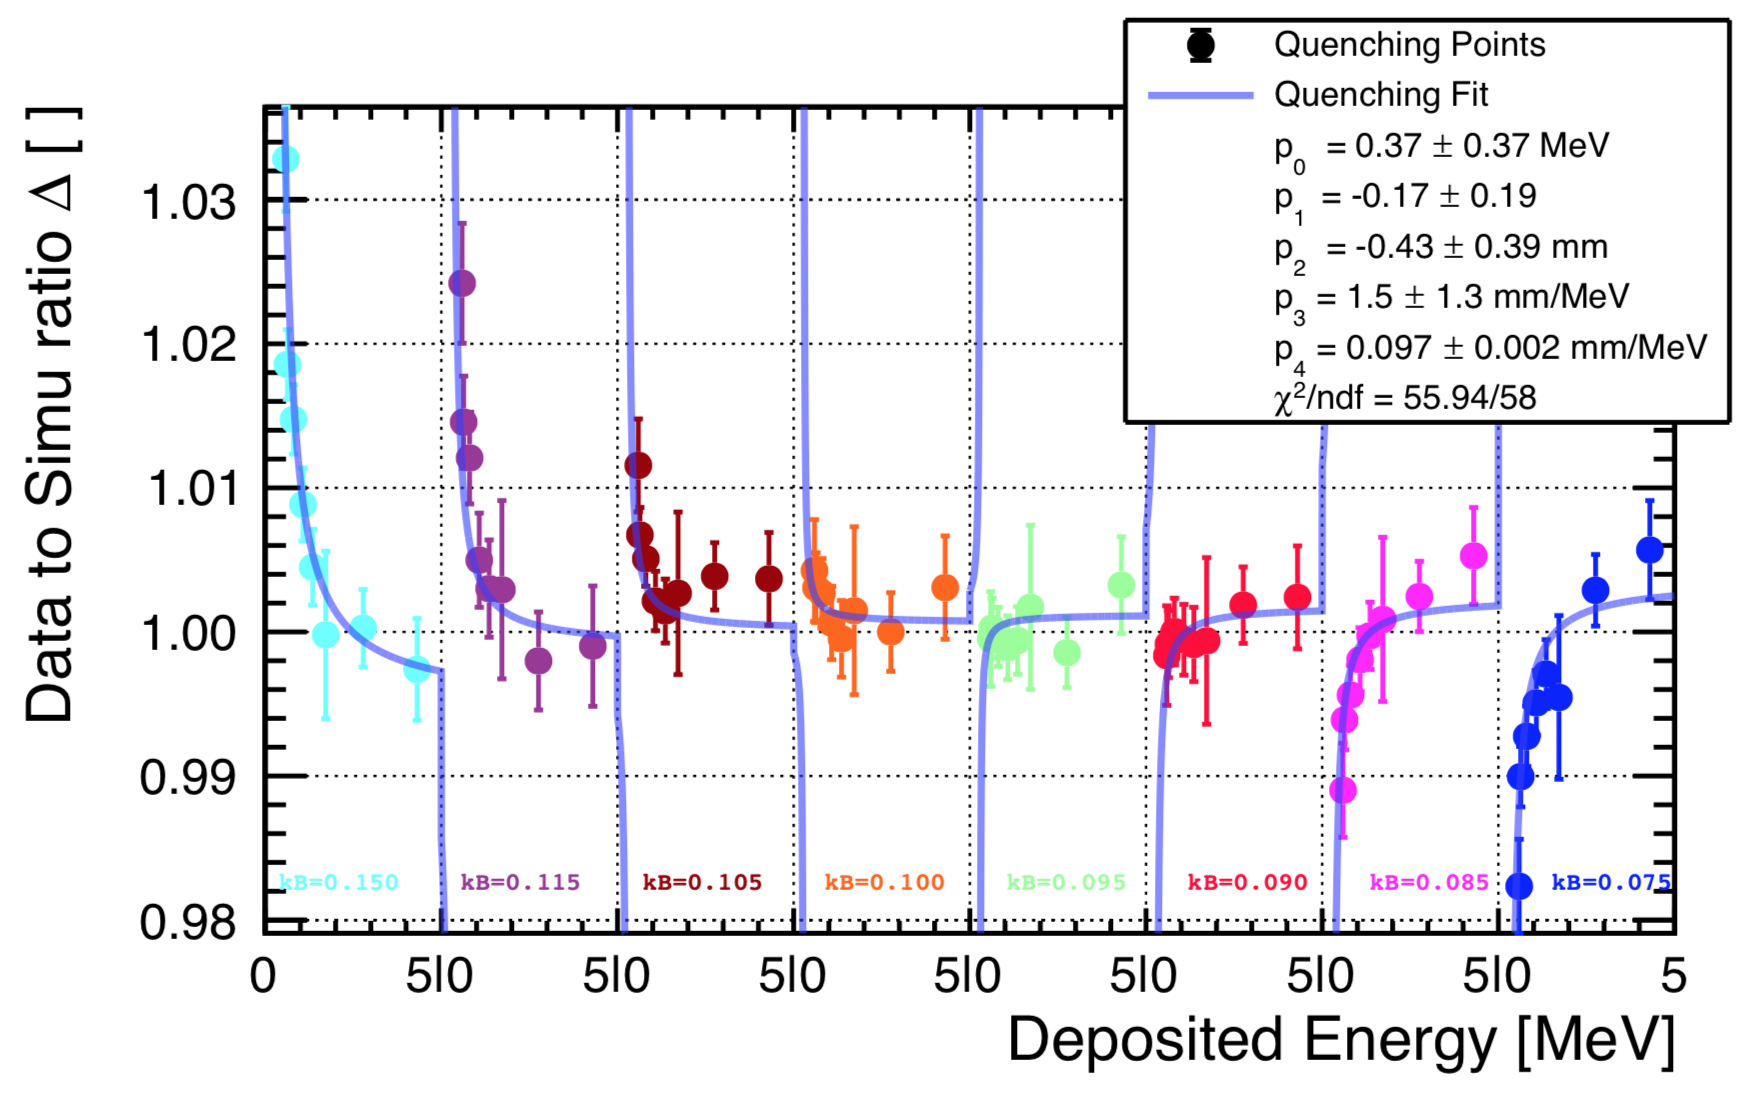
\includegraphics[width=0.8\linewidth]{images/kB_evolution.png}
  \caption[Évolution du rapport de réponse en énergie dans les données et la simulation en fonction de l'énergie des gammas et de $k_B$]{Évolution du rapport de réponse en énergie dans les données et la simulation en fonction de l'énergie des gammas et de $k_B$. Chaque couleur correspond à une valeur de $k_B$ de la simulation. À partir d'une certaine valeur de $k_B$, la pente change de sens. La valeur de $k_B^0$ optimale est choisie pour $\Delta$ soit nul sur toute la gamme en énergie. (source \cite{docdb929})}
  \label{fig:kB_evolution.png}
\end{figure}

\clearpage

}

Lorsque $k_B$ est modifié dans le MC, l'écart avec le coefficient de calibration $C_i$ des données évolue différemment avec l'énergie de la source gamma (voir figure \ref{fig:quenching_effect_on_calib}). La valeur de $k_B$ est donc ajusté pour faire correspondre les données et la simulation sur toute l'échelle en énergie. Cependant, la simulation de chaque source gamma est très coûteuse en temps de calcul et en espace disque: toutes les valeurs de $k_B$ ne peuvent pas être directement testés. Pour surmonter cette difficulté, une méthode d'estimation de $k_B$ a alors été développée.

\bigbreak

\subsection{Ajustement du quenching}
\label{sec:quenching}

$k_B$ a été ajusté de manière à faire correspondre la fonction de réponse en énergie dans les données et la simulation. Le rapport de réponse en énergie peut être exprimé en faisant apparaitre $k_B$ :

\begin{equation}
    \Delta\left(E^{\textrm{dep}}, k_B\right) \doteq \frac{E^{\textrm{rec}}_{Data}}{E^{\textrm{rec}}_{MC}\left(E^{\textrm{dep}}, k_B\right)} - 1
\end{equation}

Alternativement, cette expression peut être définie à l'aide des coefficients de calibration $C_i(E^\textrm{dep})$. On notera que $\Delta\left(E^{\textrm{dep}} = \SI{0.835}{MeV}, k_B\right) = 0$ parce que l'énergie reconstruite à été ancrée avec la source de $\ce{^{54}Mn}$. De plus, lorsque la valeur de $k_B$ est correctement ajustée la déviation donnée--simulation doit s'annuler :  $\Delta\left(E^{\textrm{dep}}, k_B = k_B^0\right) = 0$. Au premier ordre d'un développement de Taylor, l'expression de $\Delta$ devient :

\begin{equation}
    \Delta\left(E^{\textrm{dep}}, k_B\right) \simeq \left.\frac{\partial \Delta}{\partial k_B}\right|_{k_B = k_B^0} \left(k_B - k_B^0\right).
\end{equation}

\bigbreak

La dérivée de $\Delta$ par rapport à $k_B$ n'est pas connue analytiquement mais peut être approximée par une fonction ajustée sur les données. Un rapport de deux polynômes d'ordre 1 a été choisi pour effectuer cette tâche :

\begin{equation}
    \Delta\left(E^{\textrm{dep}}, k_B\right) \simeq \frac{E^{\textrm{dep}}a_1 + b_1}{E^{\textrm{dep}}a_2 + b_2} \left(k_B - k_B^0\right),
\end{equation}

où $a_1$, $b_1$, $a_2$,$b_2$ et $k_B^0$ sont des paramètres ajustés sur les données. La figure \ref{fig:kB_evolution.png} montre l'ajustement de cette fonction sur différentes simulations ayant un $k_B$ qui leur est propre.\\

% Pour que l'ajustement de $\Delta$ pointe vers la bonne valeur de $k_B^0$, il a été choisi de retirer les gammas suivants : le $\SI{2.75}{MeV}$ du $\ce{^{24}Na}$ et le $\SI{4.4}{MeV}$ de l'$\ce{AmBe}$. Les incertitudes systématiques liées à la modélisation de ces deux sources introduisent un biais sur l'ajustement de $\Delta$. En effet, le gamma de $\SI{4.4}{MeV}$ produit par l'$\ce{AmBe}$ est émis en même temps qu'un neutron rapide. Or le spectre neutron utilisé dans le MC n'est une approximation grossière. Puisque la mesure de la réponse du détecteur ne peut découpler le gamma du neutron, une erreur systématique est induite. Par ailleurs, le gamma de $\SI{2.75}{MeV}$ issu du $\ce{^{24}Na}$ donne une réponse en énergie non gaussienne, donc l'incertitude systématique sur l'extraction de la valeur du pic est large. Quoi qu'il en soit, la forme de la courbe de quenching s'aplatit à haute énergie donc les points les plus énergétiques ont peu d'influence sur l'ajustement de $\Delta$.\\


Trois analyses indépendantes ont été menées pour extraire la valeur de $k_B^0$. À la différence de la méthode employée dans le cadre de cette thèse, les équipes du MPIK et du LAPP ont estimé la valeur de $\Delta$ en mesurant l'évolution du coefficient de calibration $C_i$ pour chaque source. La valeur définitive de $k_B$ a été obtenue en faisant la moyenne des $k_B^0$ mesurés par chaque méthode :

\begin{equation}
    \overline{k_B^{0}} = (9,63 \pm 0,69)\times 10^{-2} \textrm{ mm/MeV}.
\end{equation}

\bigbreak

\afterpage{

\begin{figure}[h!]
  \centering
  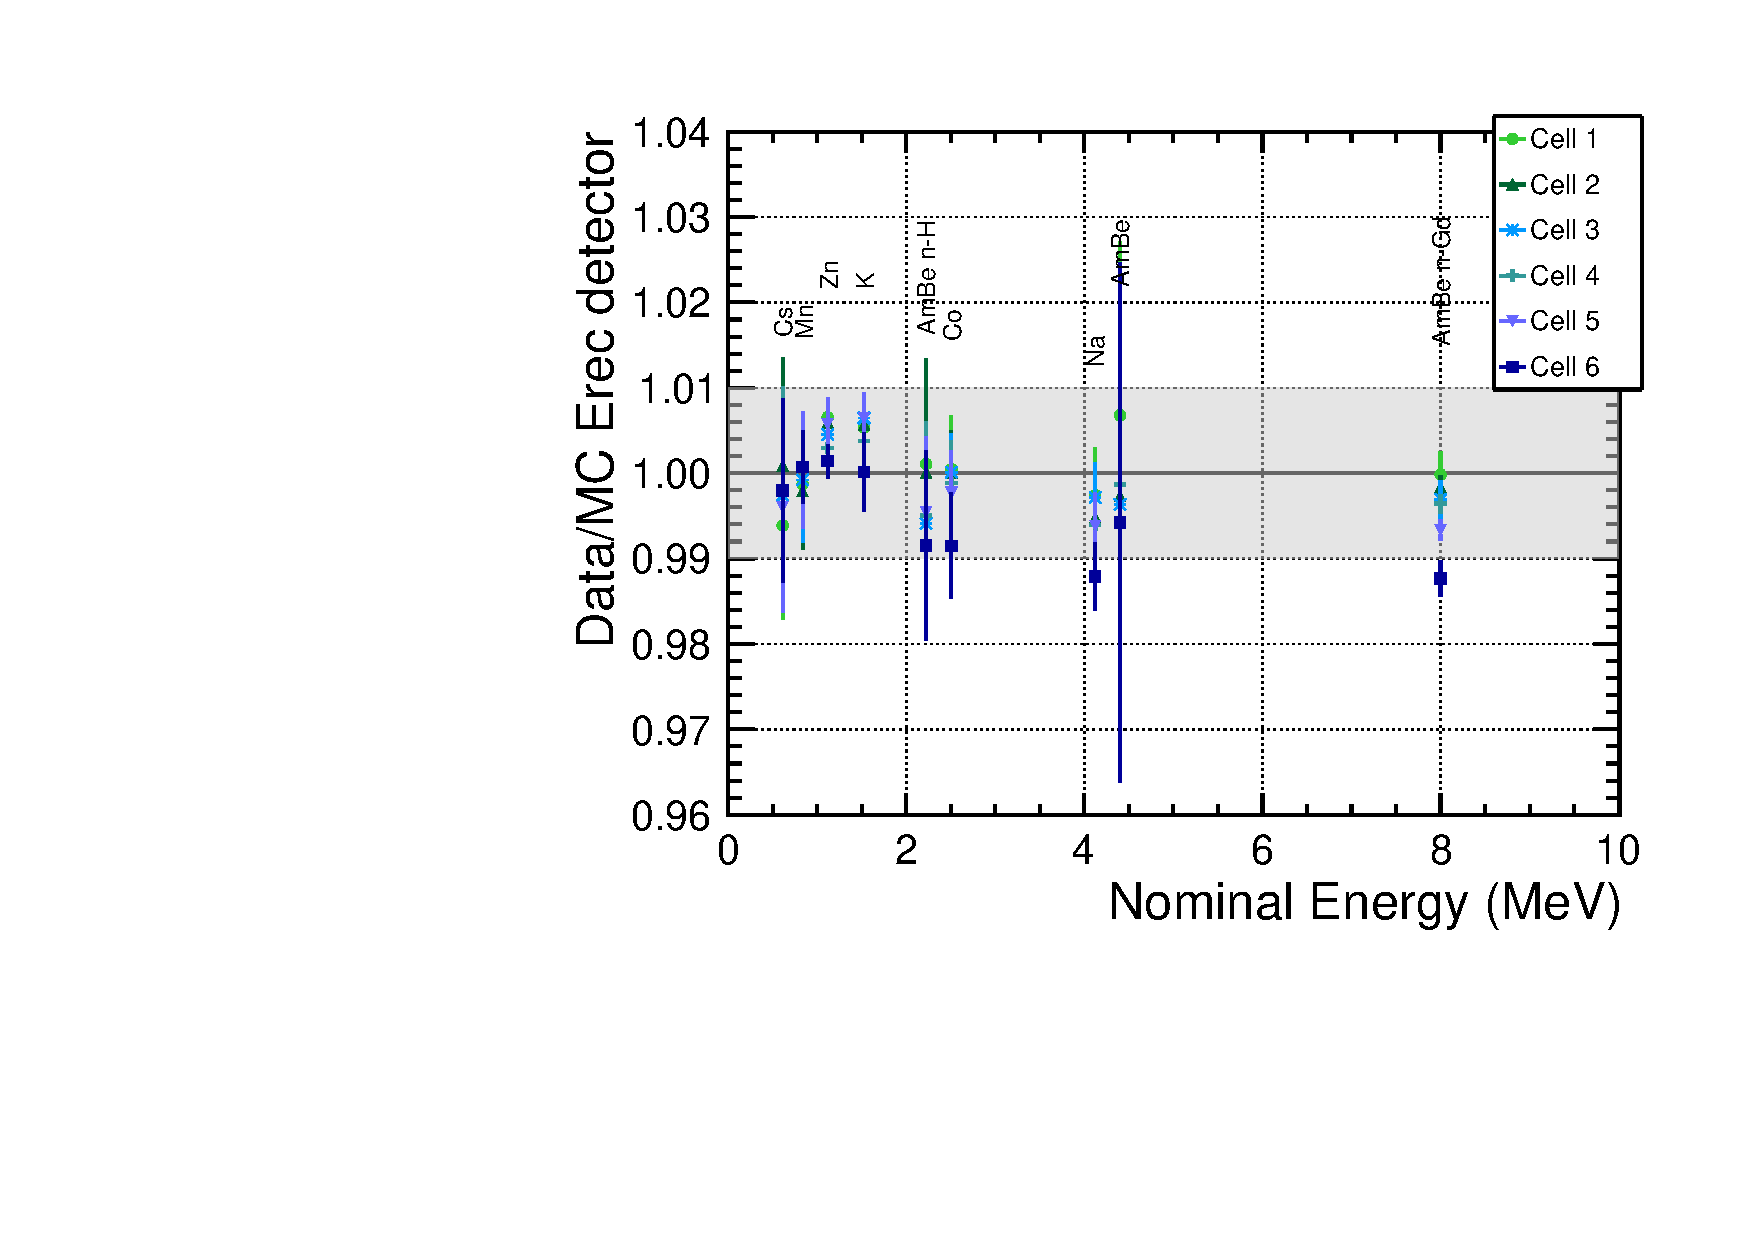
\includegraphics[width=0.8\linewidth]{images/DataMC_ErecDet_v34_meanZ_allCells.pdf}
  \caption[Test de l'échelle en énergie avec les sources de calibration]{Test de l'échelle en énergie avec les sources de calibration. Chaque point représente l'écart de la valeur des pics en énergie reconstruite entre les données et la simulation. Cette figure a été réalisée en fusionnant les runs couvrant cinq hauteurs entre 10cm et 80cm.}
  \label{fig:DataMC_ErecDet_v34_meanZ_allCells.pdf}
\end{figure}

}

Cette valeur de $k_B^0$ a permis de reproduire les effets non linéaires dans la simulation sur une échelle en énergie allant de $\SI{500}{keV}$ à $\SI{5}{MeV}$. L'écart résiduel entre les données et la simulation est présenté sur la figure \ref{fig:DataMC_ErecDet_v34_meanZ_allCells.pdf}, et montre un bon accord avec tous les points contenus dans une bande $\pm 1\%$.\\

\bigbreak

%\subsection{effets de volume}
%\label{seq:vol_effects}
%
%A FAIRE SI PLOT EST DISPO ET ADEQUATE\\
%
%Dire test quenching avec des vertex de dépot energie différents -> change pas la tete de la courbe data/MC
%
%\bigbreak

\section{Mises à l'épreuve de la méthode}
\label{seq:erec_crosscheck}

Afin de contrôler les effets systématiques résiduels sur l'énergie reconstruite, la méthode a été testée avec un jeu de données indépendant de la calibration. Les rayonnements gamma issus de captures de neutrons d'origine cosmique sont des candidats de choix pour effectuer cette mission. En effet, la répartition des vertex d'émission gamma est plus homogène que les sources de calibration et certaines cascades gamma, comme celle du $\ce{Gd}$, peuvent déposer de l'énergie dans plusieurs cellules simultanément.\\

En premier lieu, la méthode d'extraction des valeurs des pics de capture sur noyaux d'Hydrogène (n-H) et noyaux de Gadolinium (n-Gd) est présentée suivie d'une discussion sur l'évolution de la réponse en énergie du détecteur. Enfin, la comparaison avec les données cosmiques simulées est établie.\\

\subsection{Mesure des pics gamma de capture neutron}
\label{sec:pic_gamma_nH}

Puisque les gammas de capture sont induits par des neutrons d'origine cosmique, ils sont souvent précédés par un événement issu de la même gerbe. L'extraction de ces gammas dans les données est donc établie à l'aide l'algorithme de recherche de paires corrélées en temps décrit dans le Chapitre \ref{chap:chapitre_analysie}. Les sections efficaces de capture sont maximales lorsque le neutron est thermalisé. Cette phase de thermalisation dure environ $\SI{2}{\mu s}$, alors il convient de ne sélectionner que les paires séparées d'au moins cette durée. Une fois thermalisé, le neutron diffuse par collisions élastiques avec les noyaux environnants et la probabilité de capture dépend de la nature du noyau rencontré à chaque collision. Le temps moyen de capture sur l'Hydrogène est de $\SI{230}{\mu s}$ tandis que pour le Gadolinium : $\SI{16}{\mu s}$. La fenêtre de coïncidence temporelle est élargie de telle sorte à accepter plus de 90\% des captures. Enfin, les captures sur Hydrogène donnent naissance à un gamma de $\SI{2.2}{MeV}$ alors que la désexcitation du noyau de Gadolinium génère une cascade de gammas dont la somme des énergies est d'environ $\SI{8}{MeV}$. Des coupures en énergies reconstruites sont appliquées afin d'isoler ces gammas en tant qu'événements Retardés. La fenêtre Prompt quant à elle est élargie au maximum afin d'accepter tous les événements cosmiques. Cependant une énergie seuil est appliquée, car le bruit de fond accidentel devient non-négligeable à basse énergie. Les événements provoquant la saturation des PMs sont aussi retirés parce que les instabilités de la photocathode peuvent créer des candidats Retardés factices. Finalement, les coupures sur la sélection de paires sont résumées dans le Tableau \ref{tab:pair_search_cuts_for_nX_monitoring} et le principe de la recherche de paires est résumé sur la figure \ref{fig:Hcapture}.\\

\begin{figure}[h!]
  \centering
  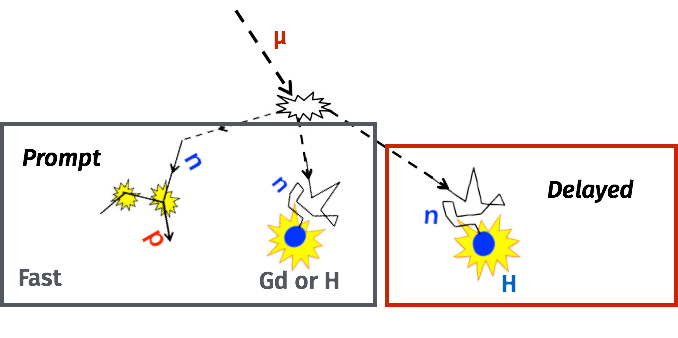
\includegraphics[width=0.8\linewidth]{images/Hcapture}
  \captionof{figure}{Méthode d'isolation des captures neutrons dans la fenêtre retardée (Delayed). Les événements qui constituent les signaux Prompts sont induits par d'autres neutrons issus du même événement cosmique. Ces neutrons peuvent être détectés par leurs collisions avec les protons du liquide (neutrons rapides), ou via la capture sur des noyaux absorbants (H ou Gd) qui se désexcitent en émettant des gammas.}
  \label{fig:Hcapture}
\end{figure}

\begin{table}[h!]
  \begin{center}
    \begin{tabular}{|l|c|c|}
      \hline
      \textbf{Candidat} & \textbf{Capture neutron} & \textbf{Coupure}\\
      \hline
      \multirow{3}{*}{Prompt} & \multirow{3}{*}{n-H et n-Gd} & $\SI{3}{MeV} < E^{\textrm{rec}}_{tot} < \SI{150}{MeV} $\\
      & & $Q_{veto} < \SI{80}{PE}$\\
      & & Saturation PMTs autorisée : Non\\
      \hline
      \multirow{5}{*}{Retardé} & \multirow{3}{*}{n-H} & $\SI{2}{\mu s} < \Delta T < \SI{300}{\mu s} $\\
      & & $\SI{1}{MeV} < E^{\textrm{rec}}_{tot} < \SI{4}{MeV} $\\
      & & $E^{\textrm{rec}}_{GC} < \SI{250}{keV}$\\
      \cline{2-3}
      & \multirow{2}{*}{n-Gd} & $\SI{2}{\mu s} < \Delta T < \SI{70}{\mu s} $\\
      & & $\SI{5}{MeV} < E^{\textrm{rec}}_{tot} < \SI{10}{MeV} $\\
      \hline
    \end{tabular}
    \caption[Liste des coupures utilisées pour la sélection des gammas de captures]{Liste des coupures utilisées pour la sélection des gammas de captures.}
    \label{tab:pair_search_cuts_for_nX_monitoring}
  \end{center}
\end{table}

Les données sont découpées par période et par cellule\footnote{L'association d'un événement à un numéro de cellule est effectuée en identifiant la cellule ayant reconstruit le plus d'énergie.} et chaque candidat de capture est stocké dans un histogramme en énergie reconstruite. Après soustraction des paires accidentelles (coïncidences fortuites, procédure décrite dans la Section \ref{seq:acc_subtraction}), la réponse en énergie reconstruite est suivie en ajustant une fonction \og Crystal Ball\fg{} qui décrit au mieux la réponse du détecteur \cite{Gaiser:1982yw} :

\begin{equation}
    \label{eq:nX_fit_function}
    f(E; B, N, \mu, \sigma, n, \alpha) = B + N \times \Gamma(E;\mu, \sigma, n, \alpha),
\end{equation}

où $B$ est un terme constant prenant en compte le bruit de fond, N un facteur de normalisation et $\Gamma$ la fonction Crystal Ball :

\begin{equation}
    \Gamma =
    \begin{cases}
        \textrm{exp}\left( - \frac{(E - \mu)^2}{2\sigma^2} \right) &\text{si $\frac{E-\mu}{\sigma} > -\alpha$},\\
        \left(\frac{n}{|\alpha|}\right)^n e^{-\alpha^2/2} \left(\frac{n}{|\alpha|} - |\alpha| - \frac{E-\mu}{\sigma}\right)^{-n} &\text{sinon.}
    \end{cases}
\end{equation}

\bigbreak

% fig:fit_example_nX.pdf

Les paramètres $\mu$ et $\sigma$ permettent de suivre respectivement la position en énergie du pic et sa largeur. Deux exemples d'ajustement montre un bon accord du modèle Crystal Ball ajusté sur les données n-H et n-Gd: figure \ref{fig:fit_example_nX.pdf}.

\afterpage{

\begin{figure}[h!]
\centering

\begin{subfigure}[b]{0.49\textwidth}
\centering
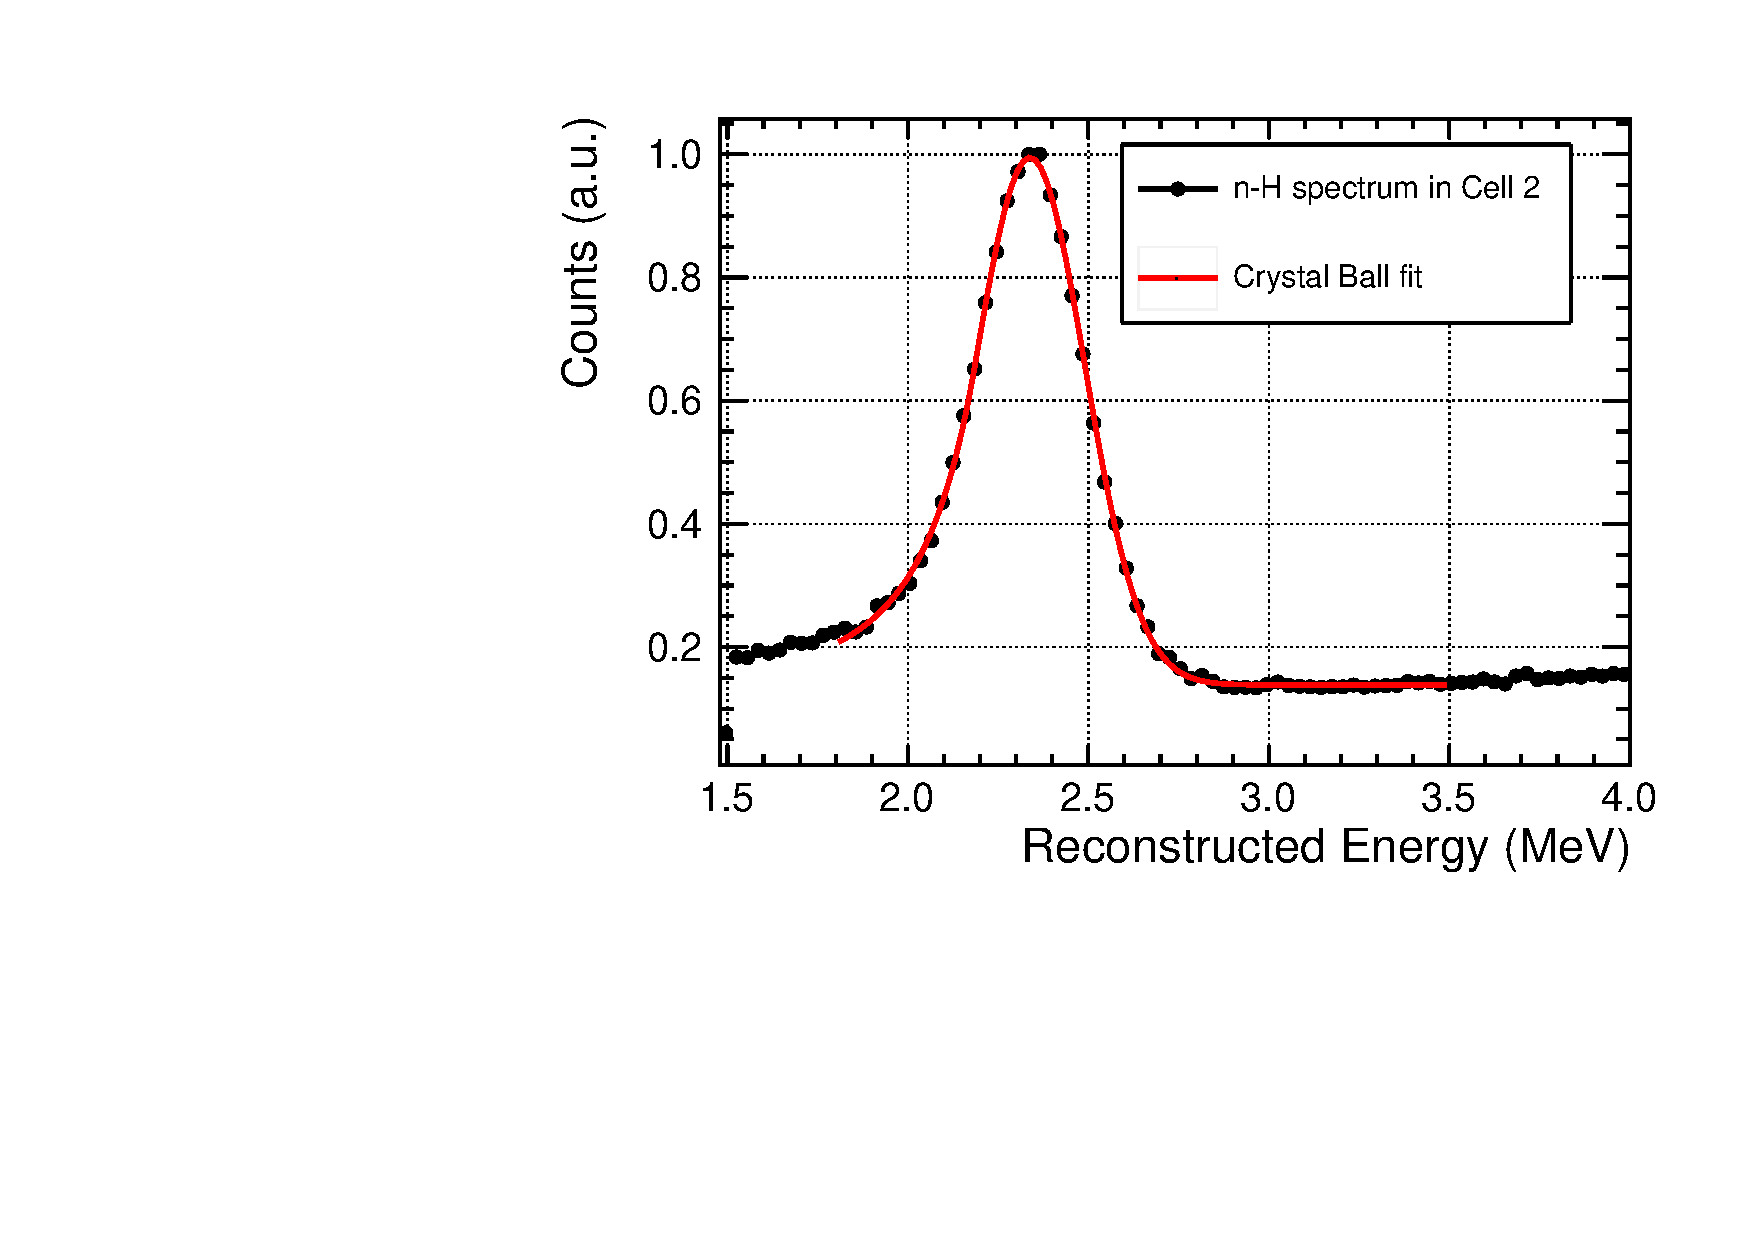
\includegraphics[width=1\textwidth]{images/fit_example_nH.pdf}
\caption{}
\label{fig:fit_example_nH.pdf}
\end{subfigure}
~ % attention ! space sensitive
\begin{subfigure}[b]{0.49\textwidth}
\centering
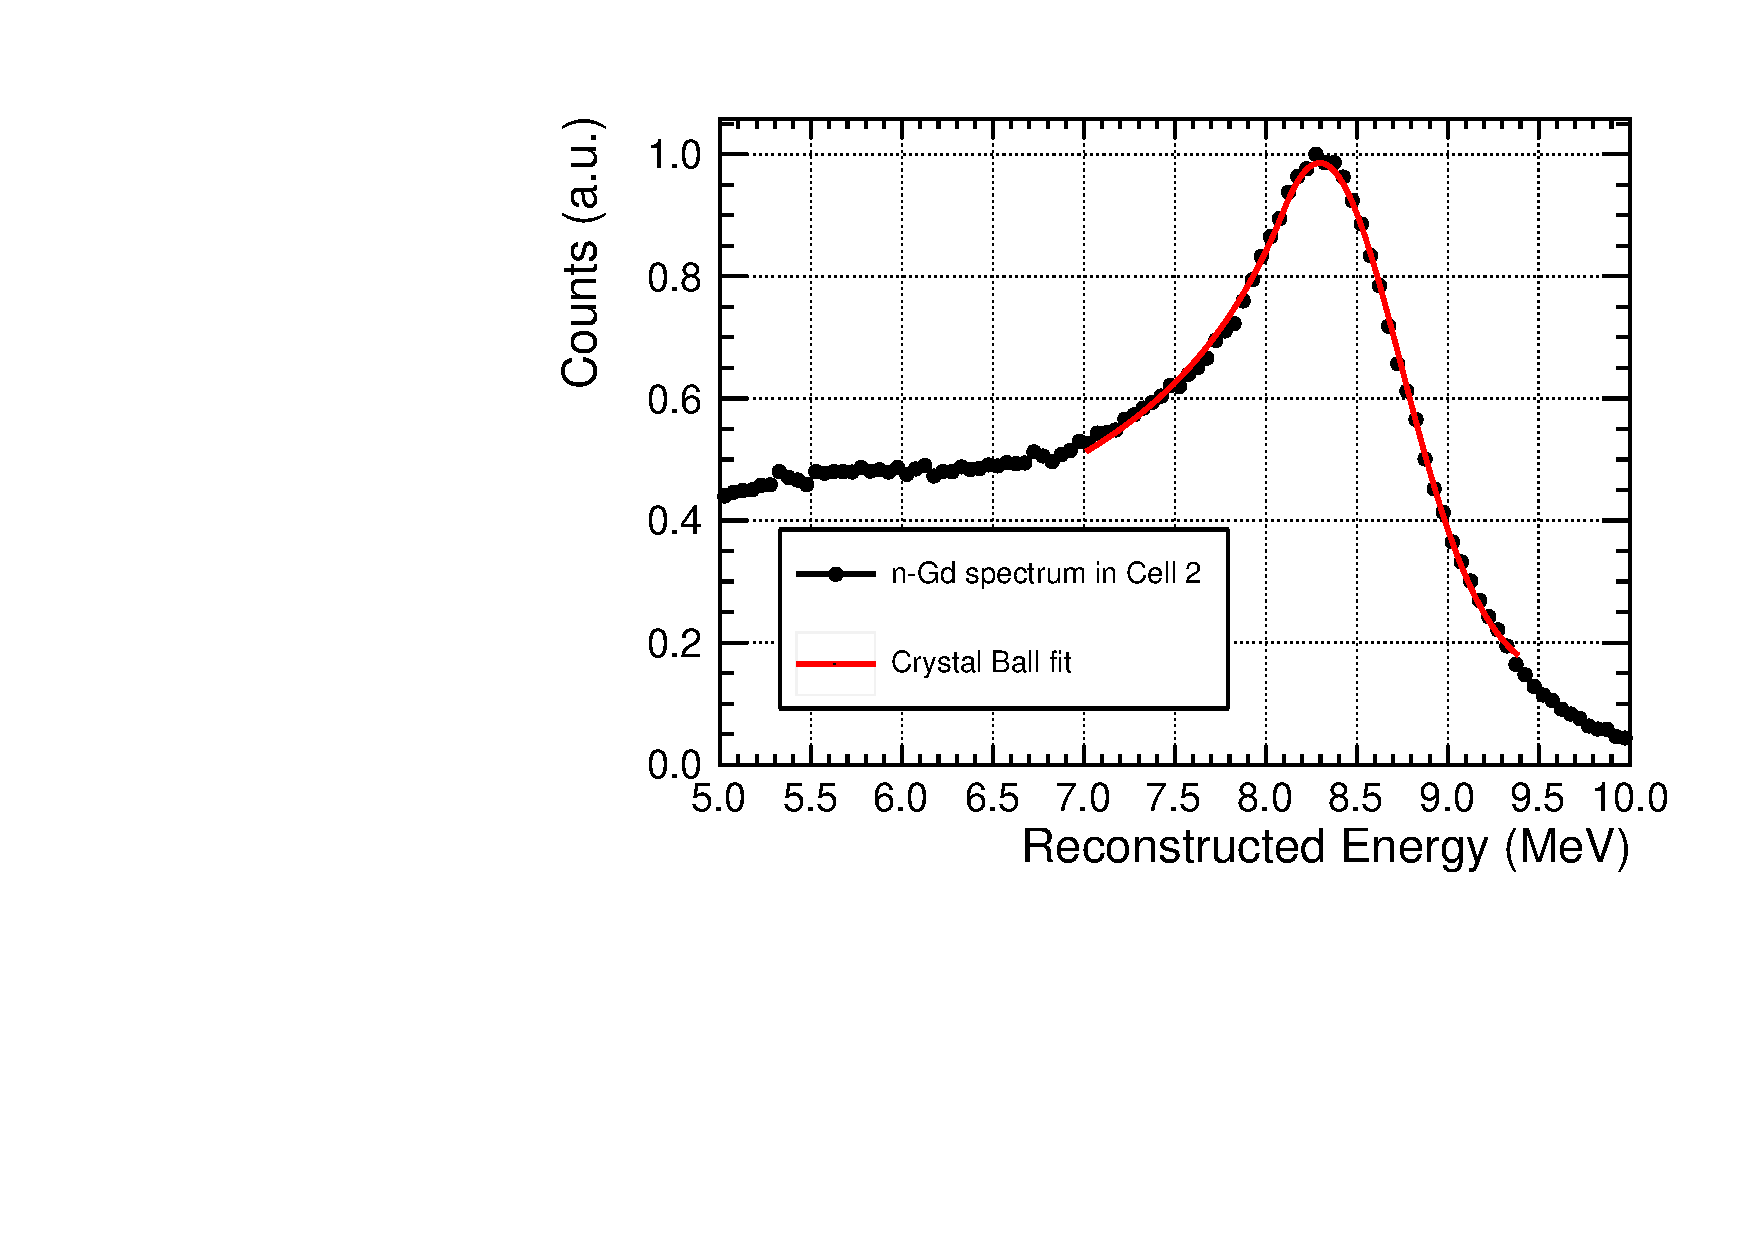
\includegraphics[width=1\textwidth]{images/fit_example_nGd.pdf}
\caption{}
\label{fig:fit_example_nGd.pdf}
\end{subfigure}

\caption[Exemple d'ajustement d'une Crystal Ball sur les pics gamma de capture neutron]{Exemple d'ajustement d'une Crystal Ball sur les pics gamma de capture neutron : n-H (a) et n-Gd (b). Les données utilisées pour former ces spectres sont issues des runs neutrinos de la phase 2.}
\label{fig:fit_example_nX.pdf}

\end{figure}


\begin{figure}[h!]
\centering

\begin{subfigure}[b]{0.49\textwidth}
\centering
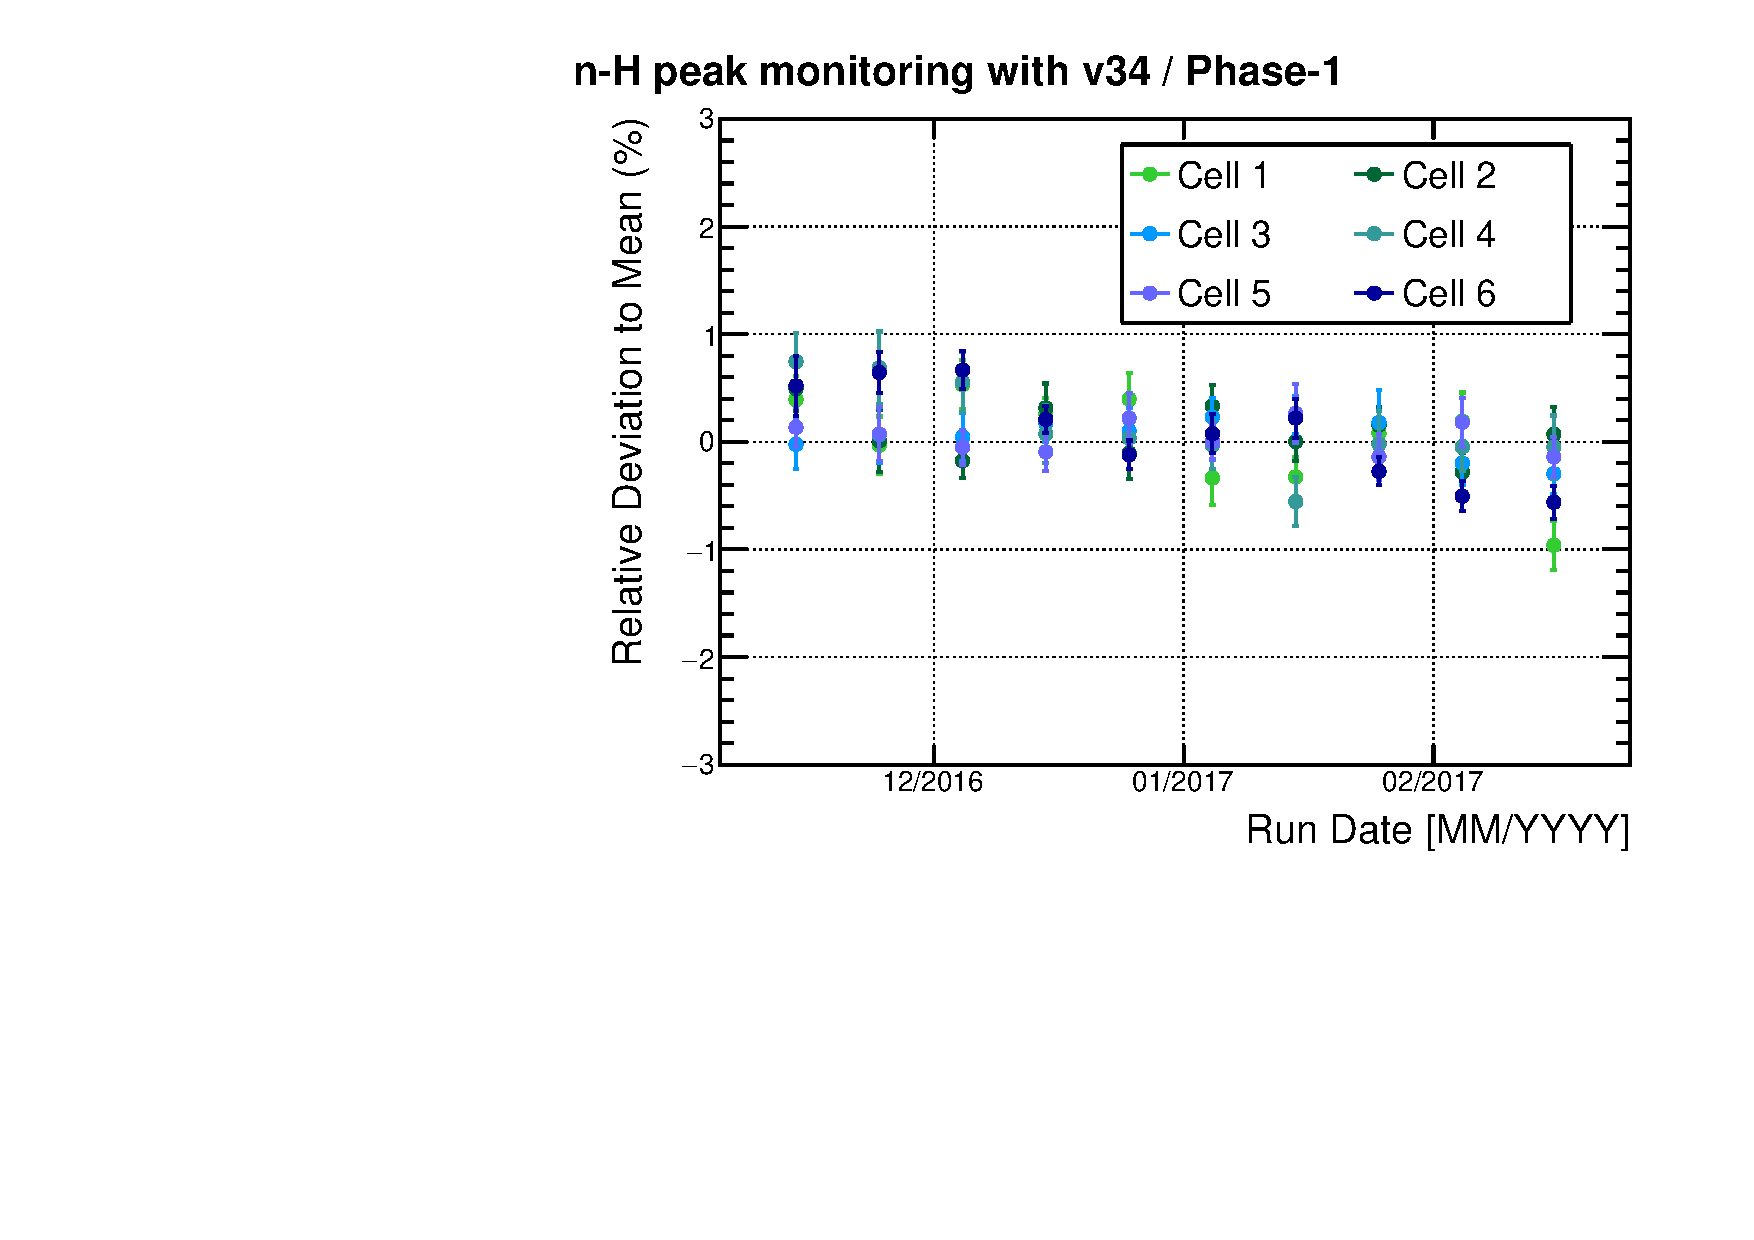
\includegraphics[width=1\textwidth]{images/Mean_peak_Erec34_nH_250GC_phase-1_fit-crystalball_stacks-10_analysis.pdf}
\caption{}
\label{fig:Mean_peak_Erec34_nH_250GC_phase-1_fit-crystalball_stacks-10_analysis.pdf}
\end{subfigure}


%~ % attention ! space sensitive
\begin{subfigure}[b]{0.49\textwidth}
\centering
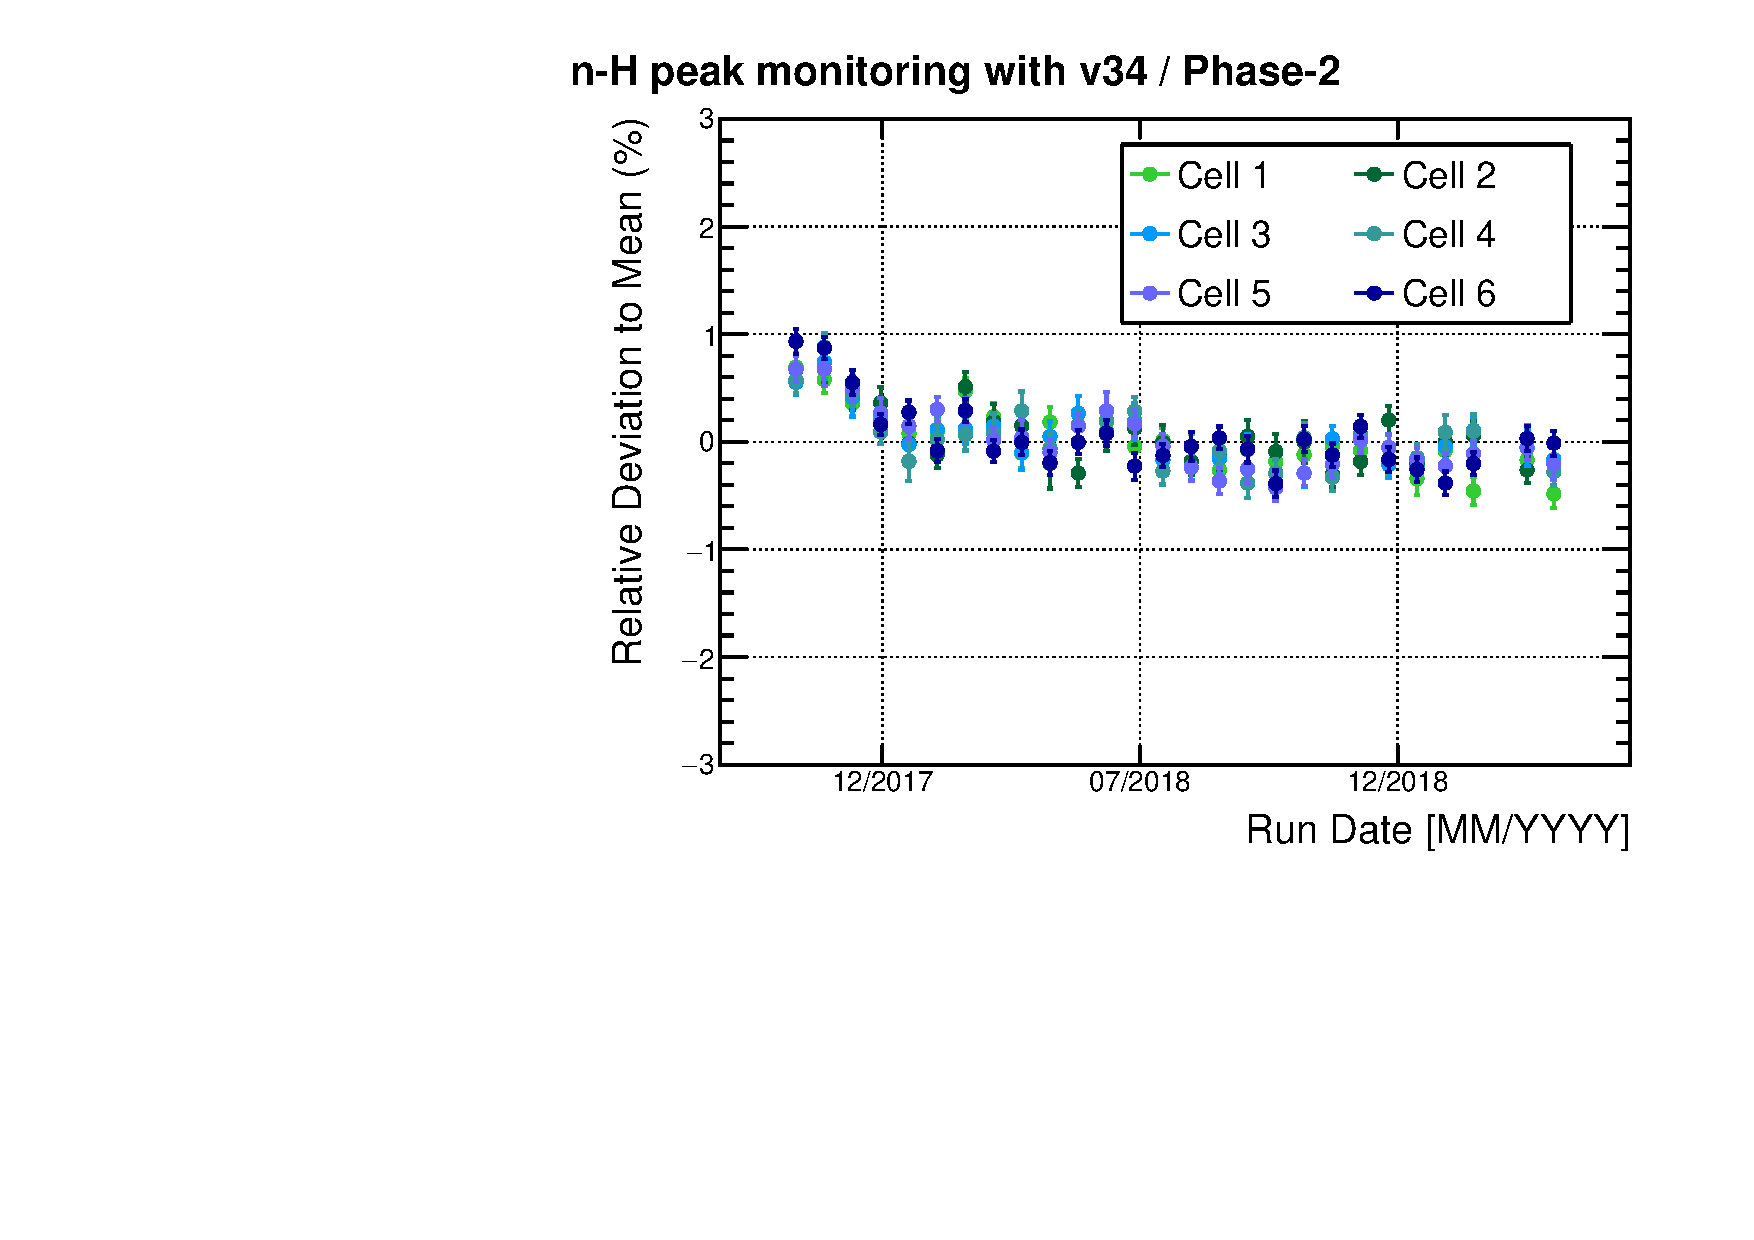
\includegraphics[width=1\textwidth]{images/Mean_peak_Erec34_nH_250GC_phase-2_fit-crystalball_stacks-20_analysis.pdf}
\caption{}
\label{fig:Mean_peak_Erec34_nH_250GC_phase-2_fit-crystalball_stacks-20_analysis.pdf}
\end{subfigure}
~ % attention ! space sensitive
\begin{subfigure}[b]{0.49\textwidth}
\centering
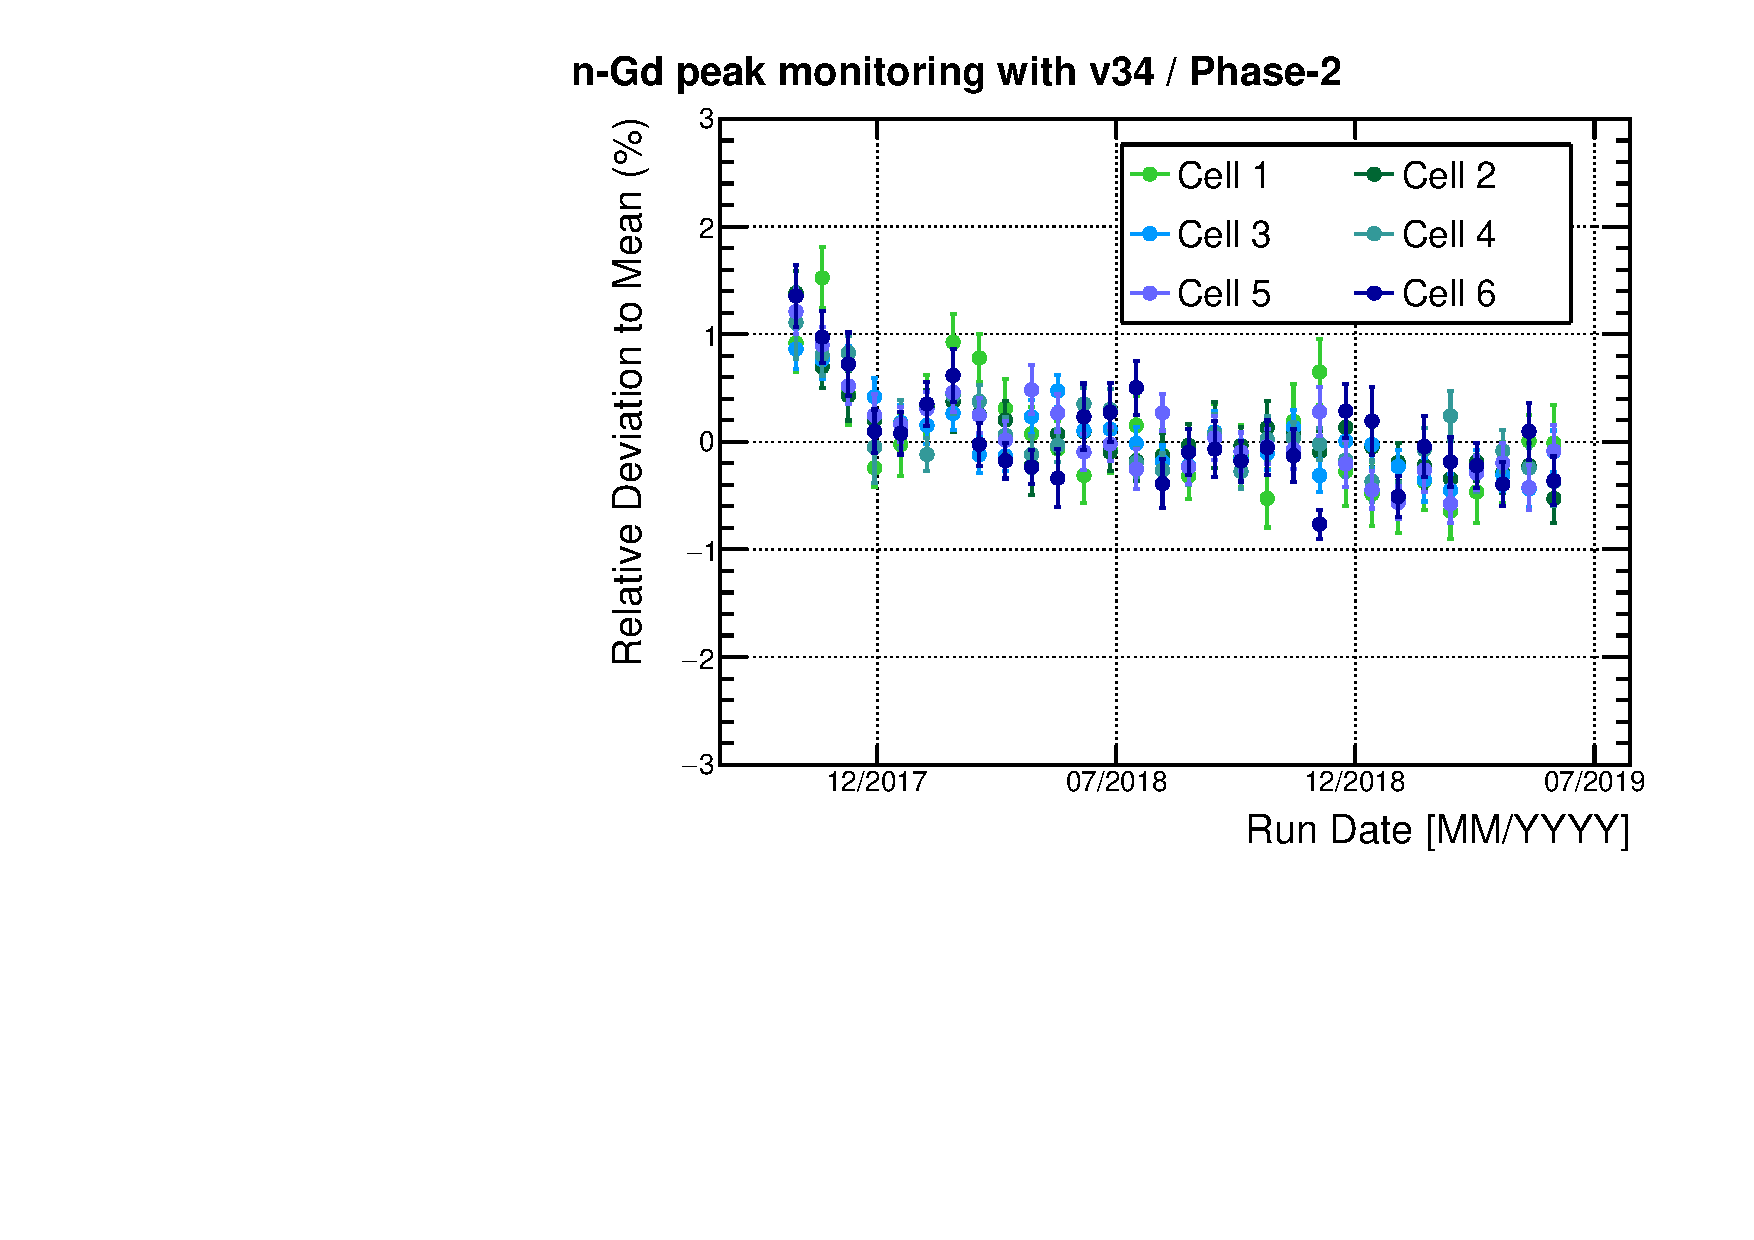
\includegraphics[width=1\textwidth]{images/Erec34_nGd_phase-2_fit-crystalball_stacks-20_analysis.pdf}
\caption{}
\label{fig:Erec34_nGd_phase-2_fit-crystalball_stacks-20_analysis.pdf}
\end{subfigure}


\caption[Évolution relative des pics gamma de capture neutronique]{Évolution relative des pics gamma de capture neutronique. (a) représente le suivi du pic n-H pendant la phase 1. Chaque point rassemble 10 jours de prise de données. (b) montre l'évolution du pic n-H en phase 2. Cette fois chaque point rassemble 20 jours de prise de données. (c) illustre l'évolution de la position du pic n-Gd pendant la phase 2. Chaque point rassemble également 20 jours de données.}
\label{fig:nX_relative_evol}

\end{figure}

\clearpage

}

\afterpage{

\begin{figure}[h!]
  \centering
  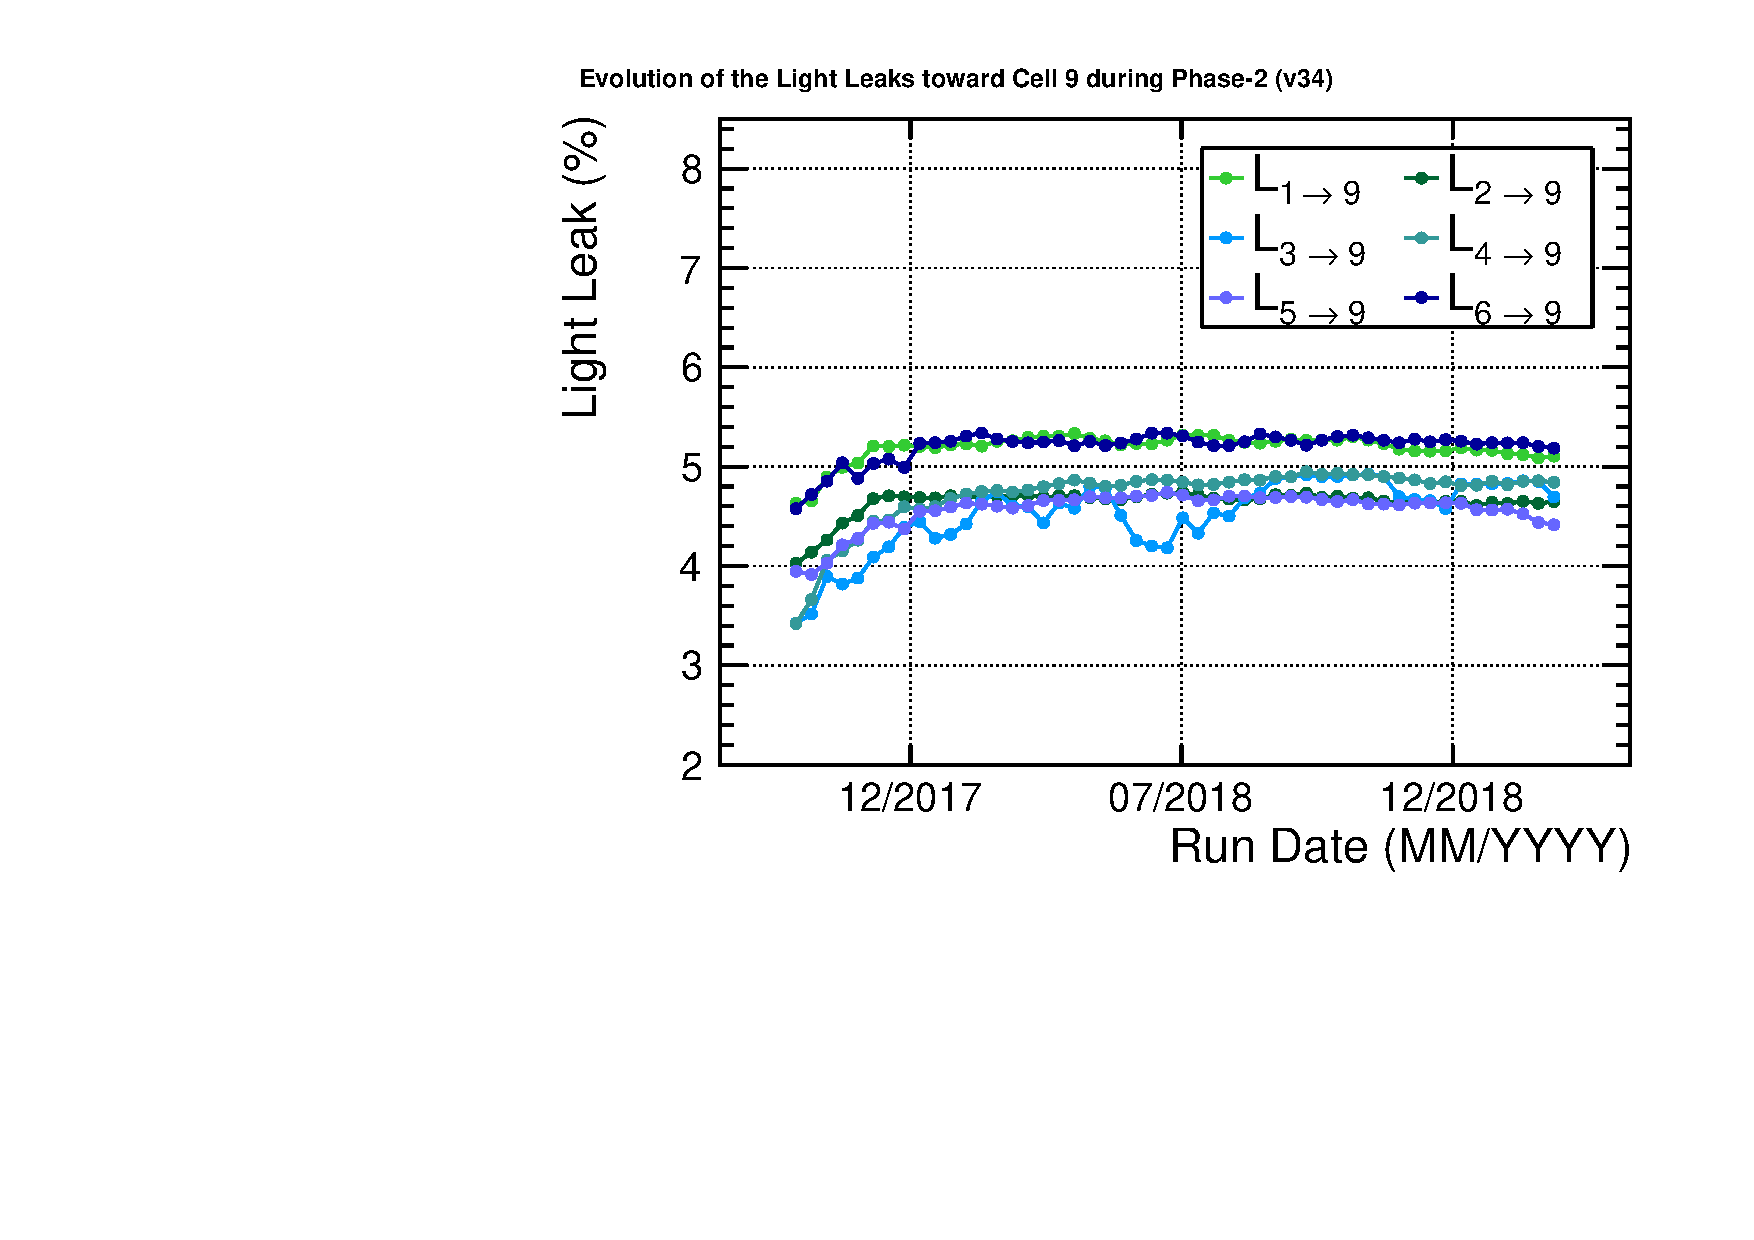
\includegraphics[width=0.8\linewidth]{images/LL_T_to_9_p2.pdf}
  \caption[Suivi des fuites de lumière vers la cellule 9 (Gamma-Catcher côté IN20)]{Suivi des fuites de lumière vers la cellule 9 (Gamma-Catcher côté IN20). L'augmentation brusque des fuites de lumière vers la cellule 9 est un candidat potentiel pour expliquer l'évolution des pics n-H et n-Gd en début de phase 2.}
  \label{fig:LL_T_to_9_p2.pdf}
\end{figure}


\begin{figure}[h!]
\centering

%~ % attention ! space sensitive
\begin{subfigure}[b]{0.49\textwidth}
\centering
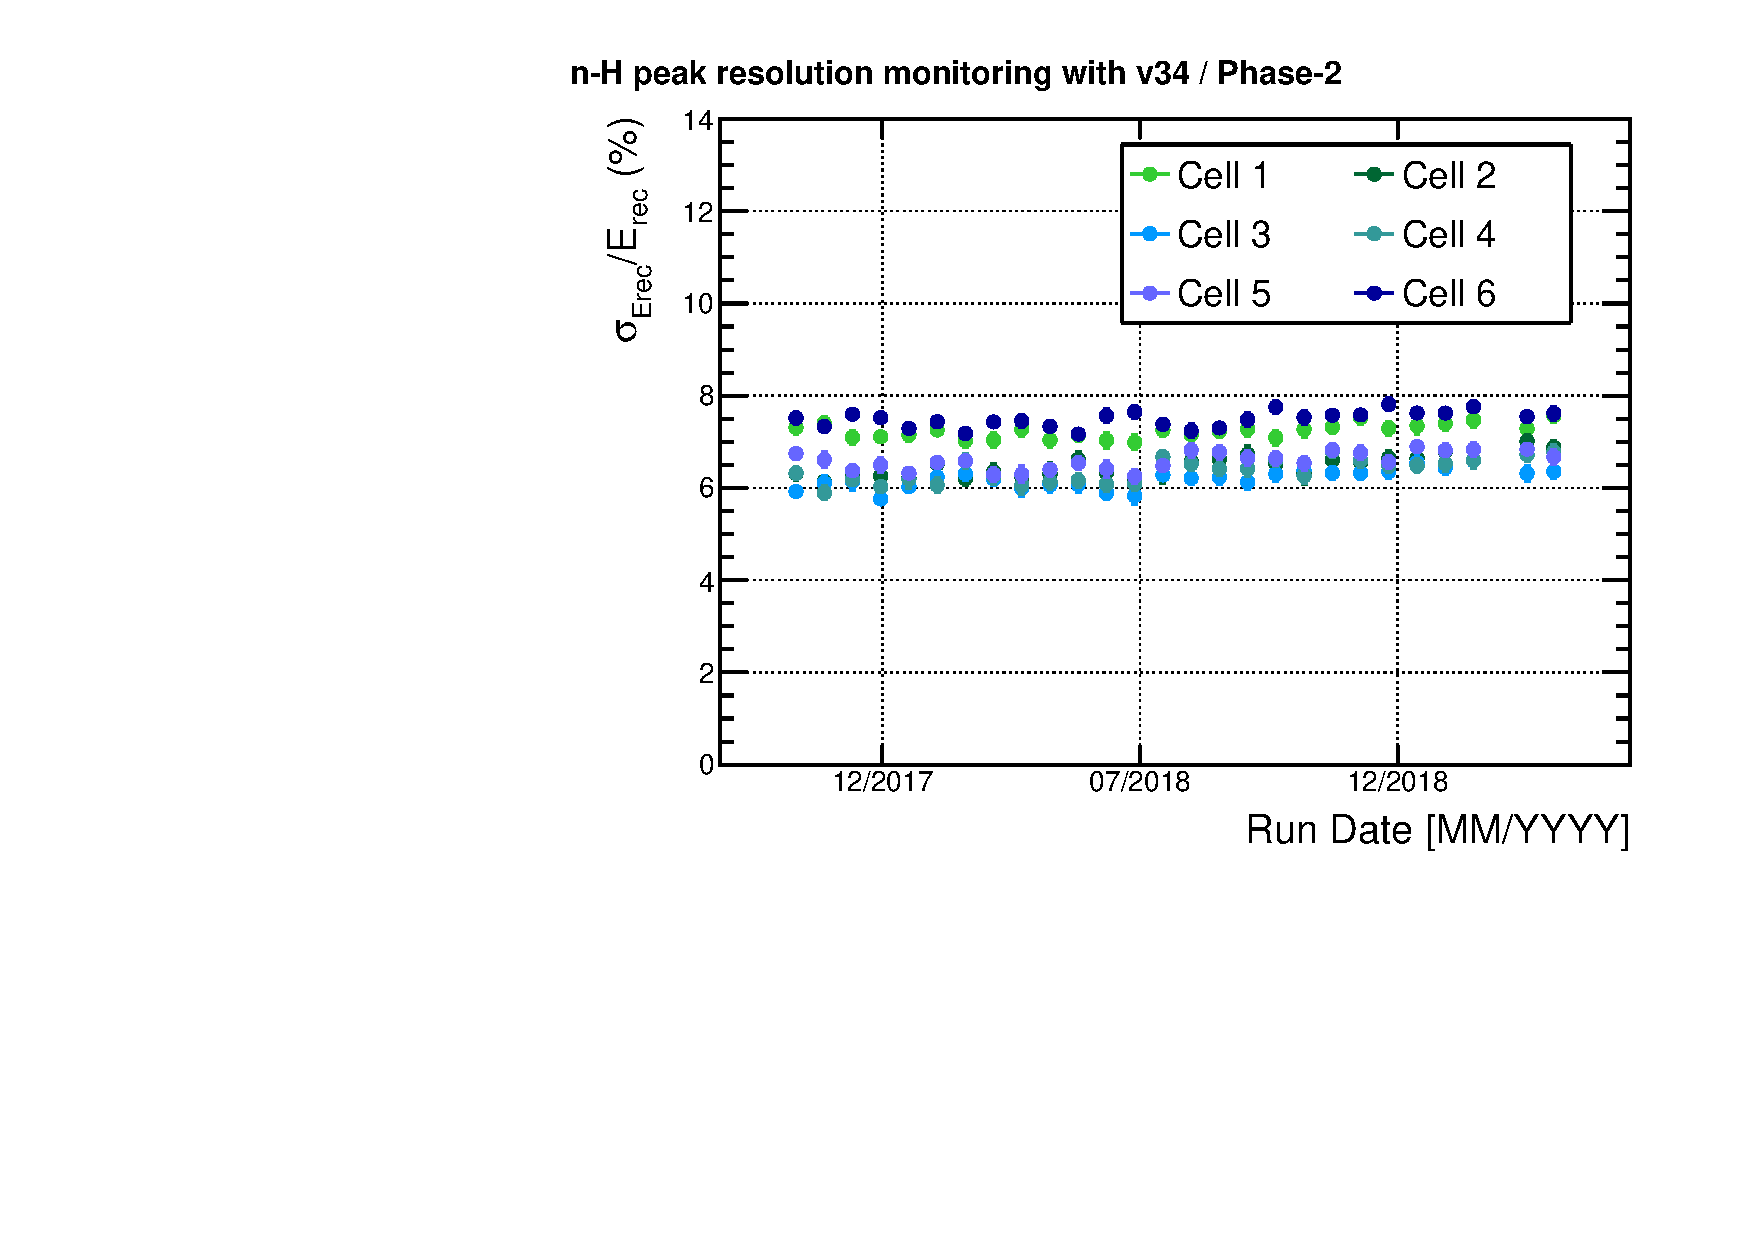
\includegraphics[width=1\textwidth]{images/Sigma_peak_Erec34_nH_250GC_phase-2_fit-crystalball_stacks-20_analysis.pdf}
\caption{}
\label{fig:Sigma_peak_Erec34_nH_250GC_phase-2_fit-crystalball_stacks-20_analysis.pdf}
\end{subfigure}
~ % attention ! space sensitive
\begin{subfigure}[b]{0.49\textwidth}
\centering
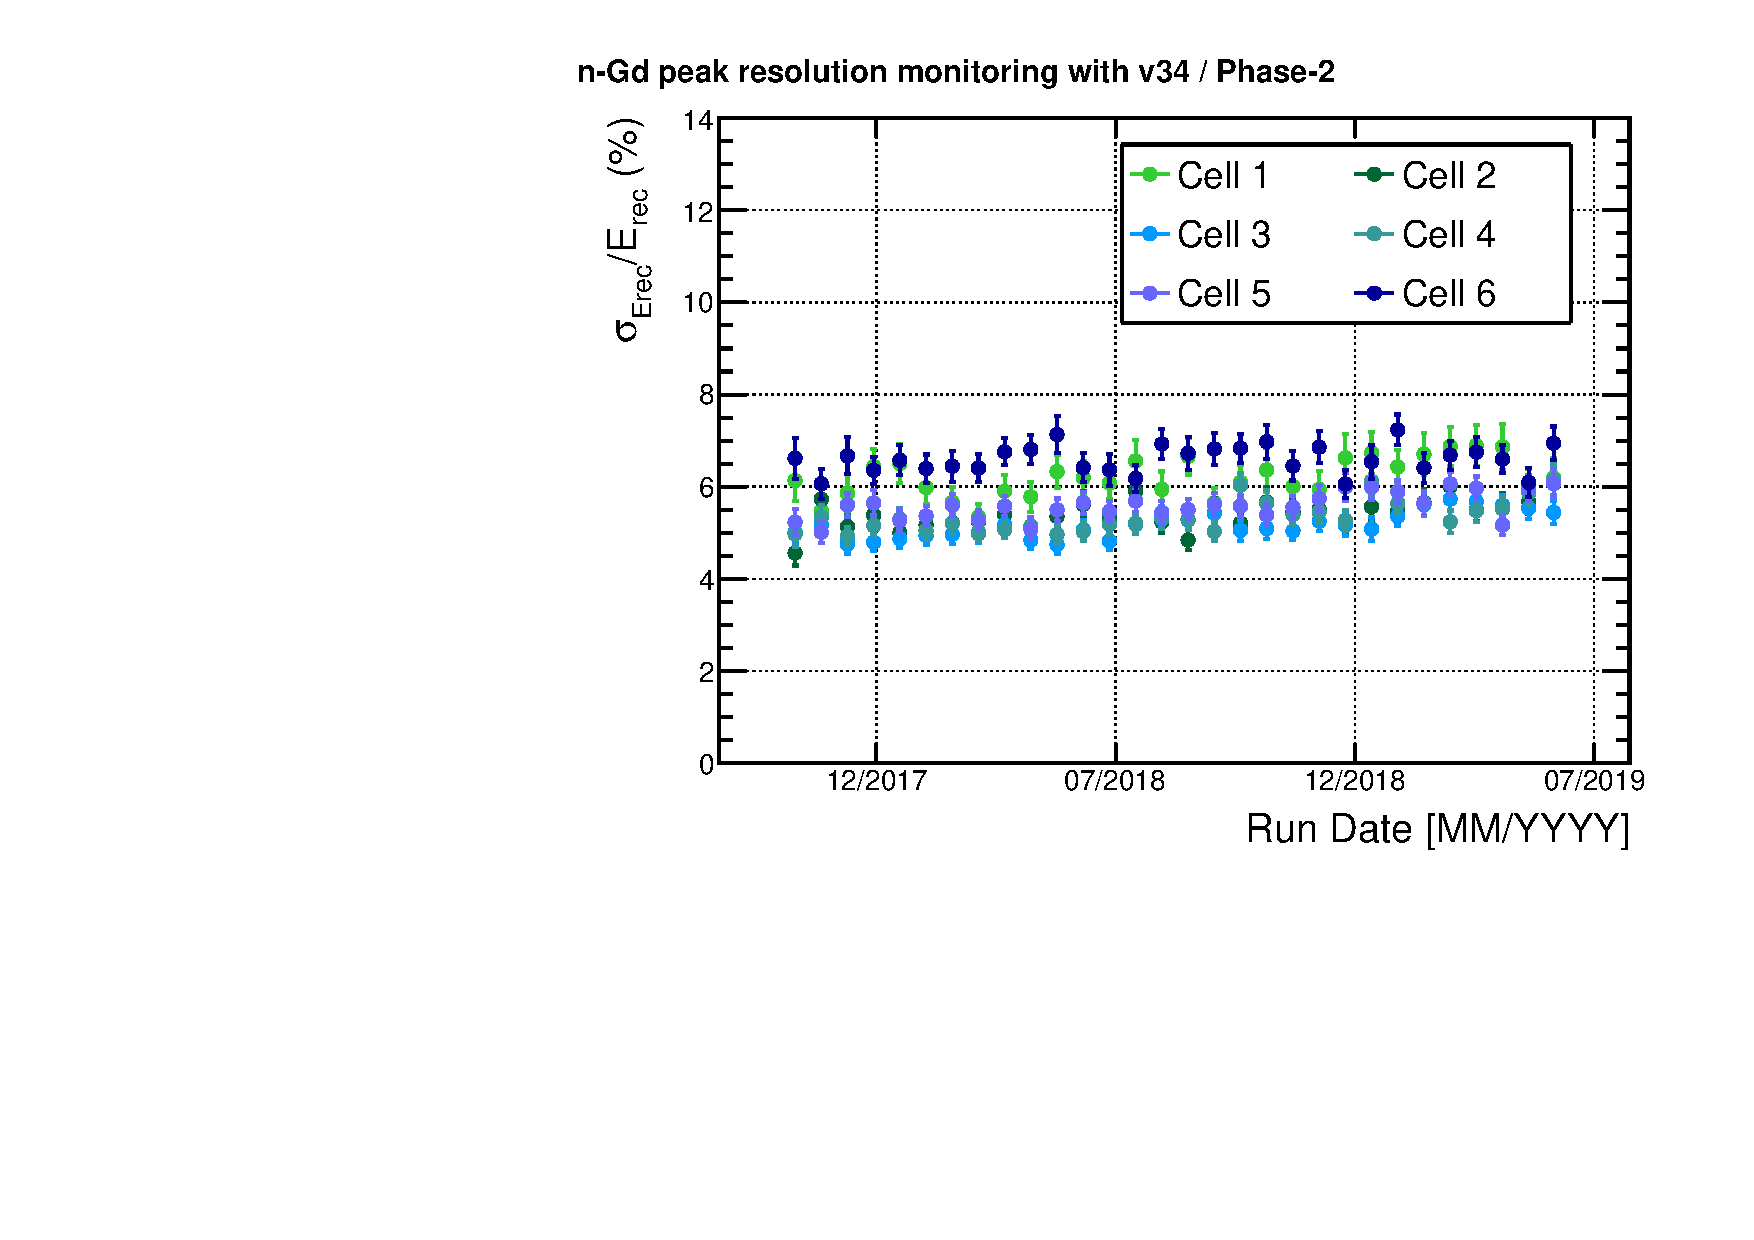
\includegraphics[width=1\textwidth]{images/Sigma_peak_Erec34_nGd_phase-2_fit-crystalball_stacks-20_analysis.pdf}
\caption{}
\label{fig:Sigma_peak_Erec34_nGd_phase-2_fit-crystalball_stacks-20_analysis.pdf}
\end{subfigure}


\caption[Évolution de la résolution des pics de captures neutron]{Évolution de la résolution des pics de captures neutron. La résolution est définie comme le rapport de la largeur du pic (composante gaussienne de la Crystal-Ball) sur l'énergie du pic. (a) montre l'évolution de la résolution pour le pic n-H et (b) représente celle du n-Gd.}
\label{fig:nX_resolution_evol}

\end{figure}

}

\subsection{Suivi de la réponse du détecteur}

Les données n-H et n-Gd offrent un moyen de suivre la réponse du détecteur avec des distributions de dépôts d'énergie similaires à ceux des neutrinos. Les variations relatives de la valeur la plus probable des spectres ($\mu$) sont présentées sur la figure \ref{fig:nX_relative_evol}.\\

En phase 1, la valeur moyenne du pic n-H est stable à $\pm 0.5\%$ près pour toutes les cellules (voire figure \ref{fig:Mean_peak_Erec34_nH_250GC_phase-1_fit-crystalball_stacks-10_analysis.pdf}). Les cellules 1 et 6 présentent néanmoins une légère dépendance en temps sur toute la période. Ces évolutions résiduelles ont été attribuées à l'accroissement des fuites de lumière. En effet, en plus de réduire les performances des parois réfléchissantes, la pénétration du liquide scintillateur dans les sandwichs en acrylique fait évoluer l'asymétrie haut-bas sur la collection de lumière. Puisque les dépôts d'énergies des événements n-H ont davantage lieu en bas des cellules (cf. Section \ref{sec:sim_gamma_from_nX}) et que la calibration utilisée pour reconstruire les pics est ajustée sur des événements $\ce{^{54}Mn}$ équirépartis en Z, le pic n-H est sensible aux variations relatives des effets haut-bas.\\

En comparaison, la phase 2 présente une tendance décroissante visible à la fois sur les données n-H (fig. \ref{fig:Mean_peak_Erec34_nH_250GC_phase-2_fit-crystalball_stacks-20_analysis.pdf}) et n-Gd (\ref{fig:Erec34_nGd_phase-2_fit-crystalball_stacks-20_analysis.pdf}) entre début novembre 2017 et fin décembre 2017. Celle-ci coïncide avec le développement des fuites de lumière vers la cellule 9 (longue cellule du Gamma-Catcher, côté IN20) comme le montre la figure \ref{fig:LL_T_to_9_p2.pdf}. La brusque diminution de la réponse en énergie des pics de capture neutron est probablement dû à l'accroissement des fuites de lumière vers le Gamma-Catcher. Par ailleurs, la tendance décroissance globale après cette période est en accord avec l'hypothèse de la lente dégradation du liquide scintillateur (cf. Section \ref{sec:cc_encrage}). Une diminution sensible de la longueur d'atténuation du liquide pourrait expliquer cet effet.\\

\afterpage{

\begin{figure}[h!]
\centering

\begin{subfigure}[b]{0.49\textwidth}
\centering
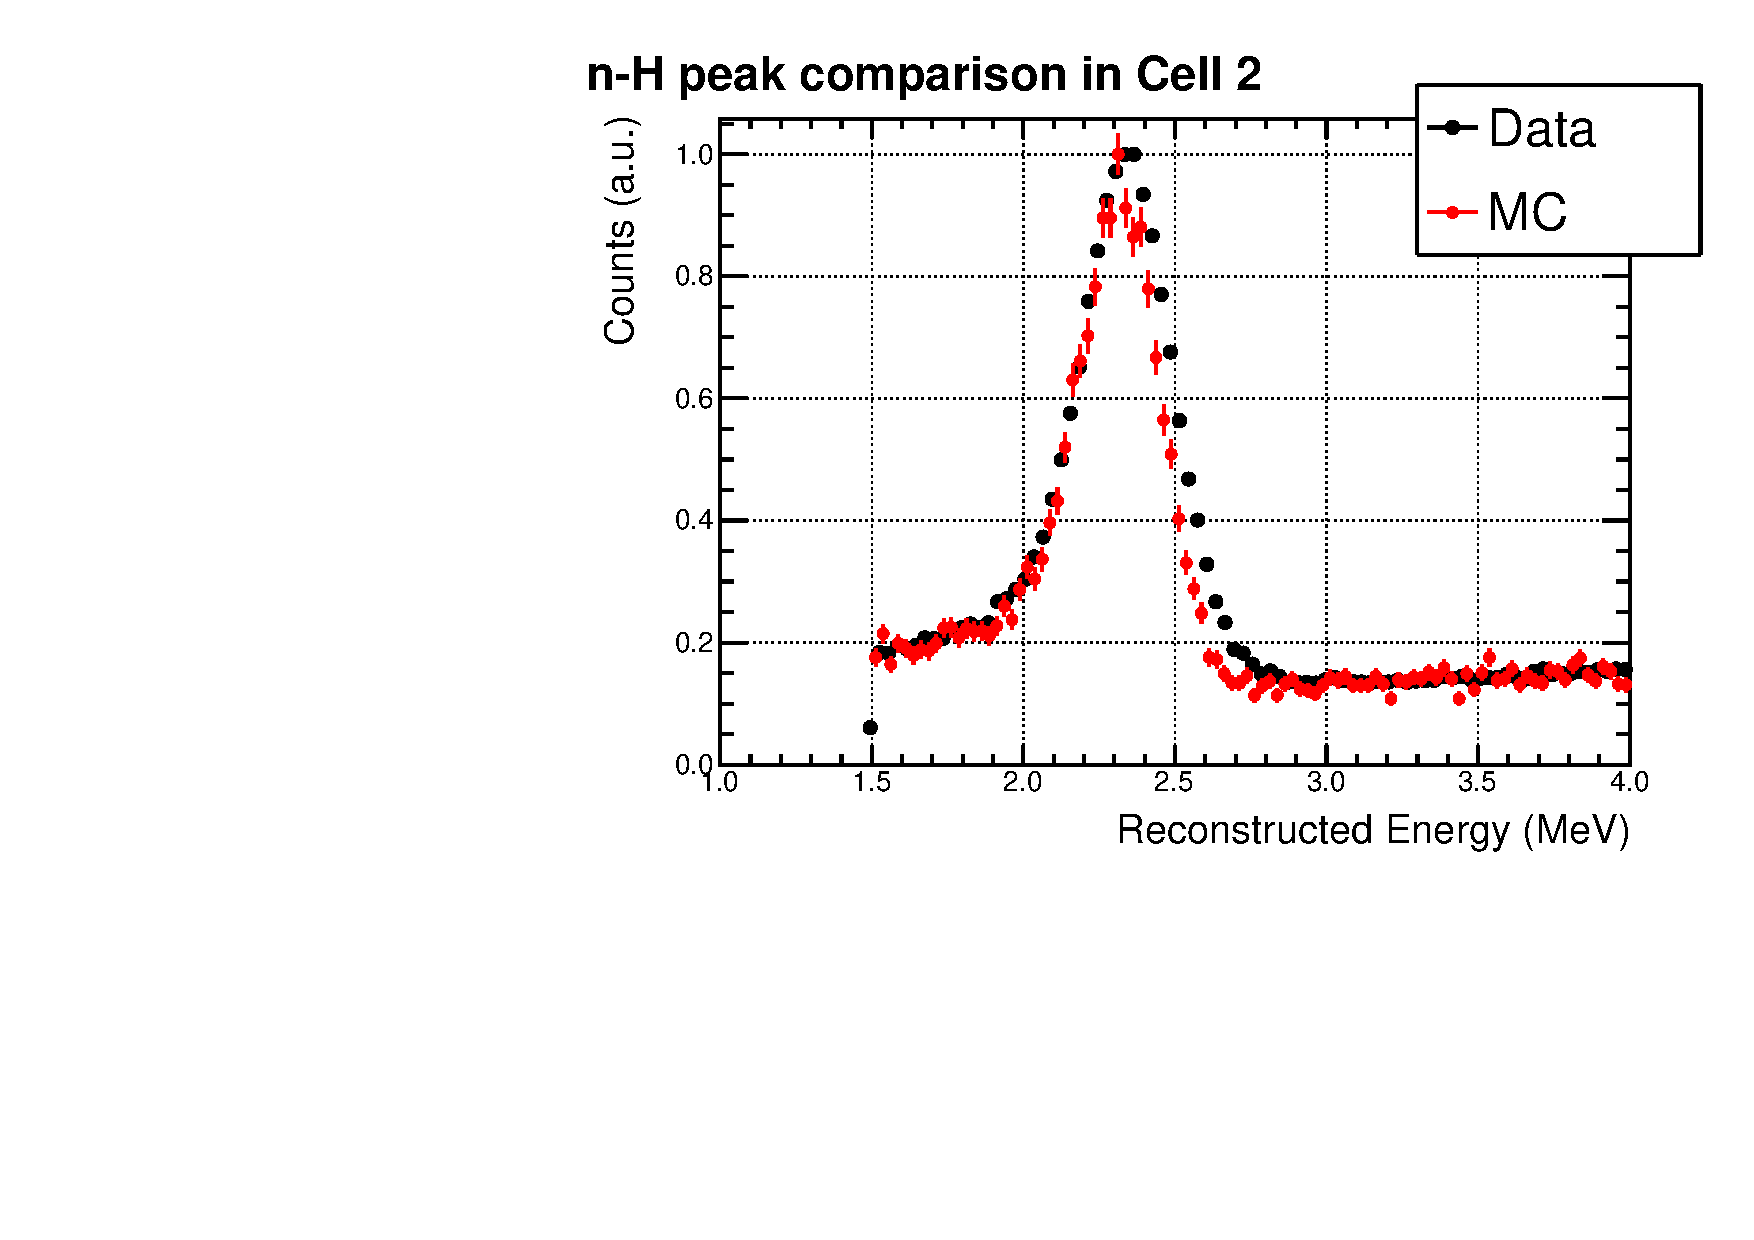
\includegraphics[width=1\textwidth]{images/Data_MC_peak_comparison_Cell2_Erec34_nH_250GC_phase-2_fit-crystalball_stacks-20_analysis.pdf}
\caption{}
\label{fig:Data_MC_peak_comparison_Cell2_Erec34_nH_250GC_phase-2_fit-crystalball_stacks-20_analysis.pdf}
\end{subfigure}
~ % attention ! space sensitive
\begin{subfigure}[b]{0.49\textwidth}
\centering
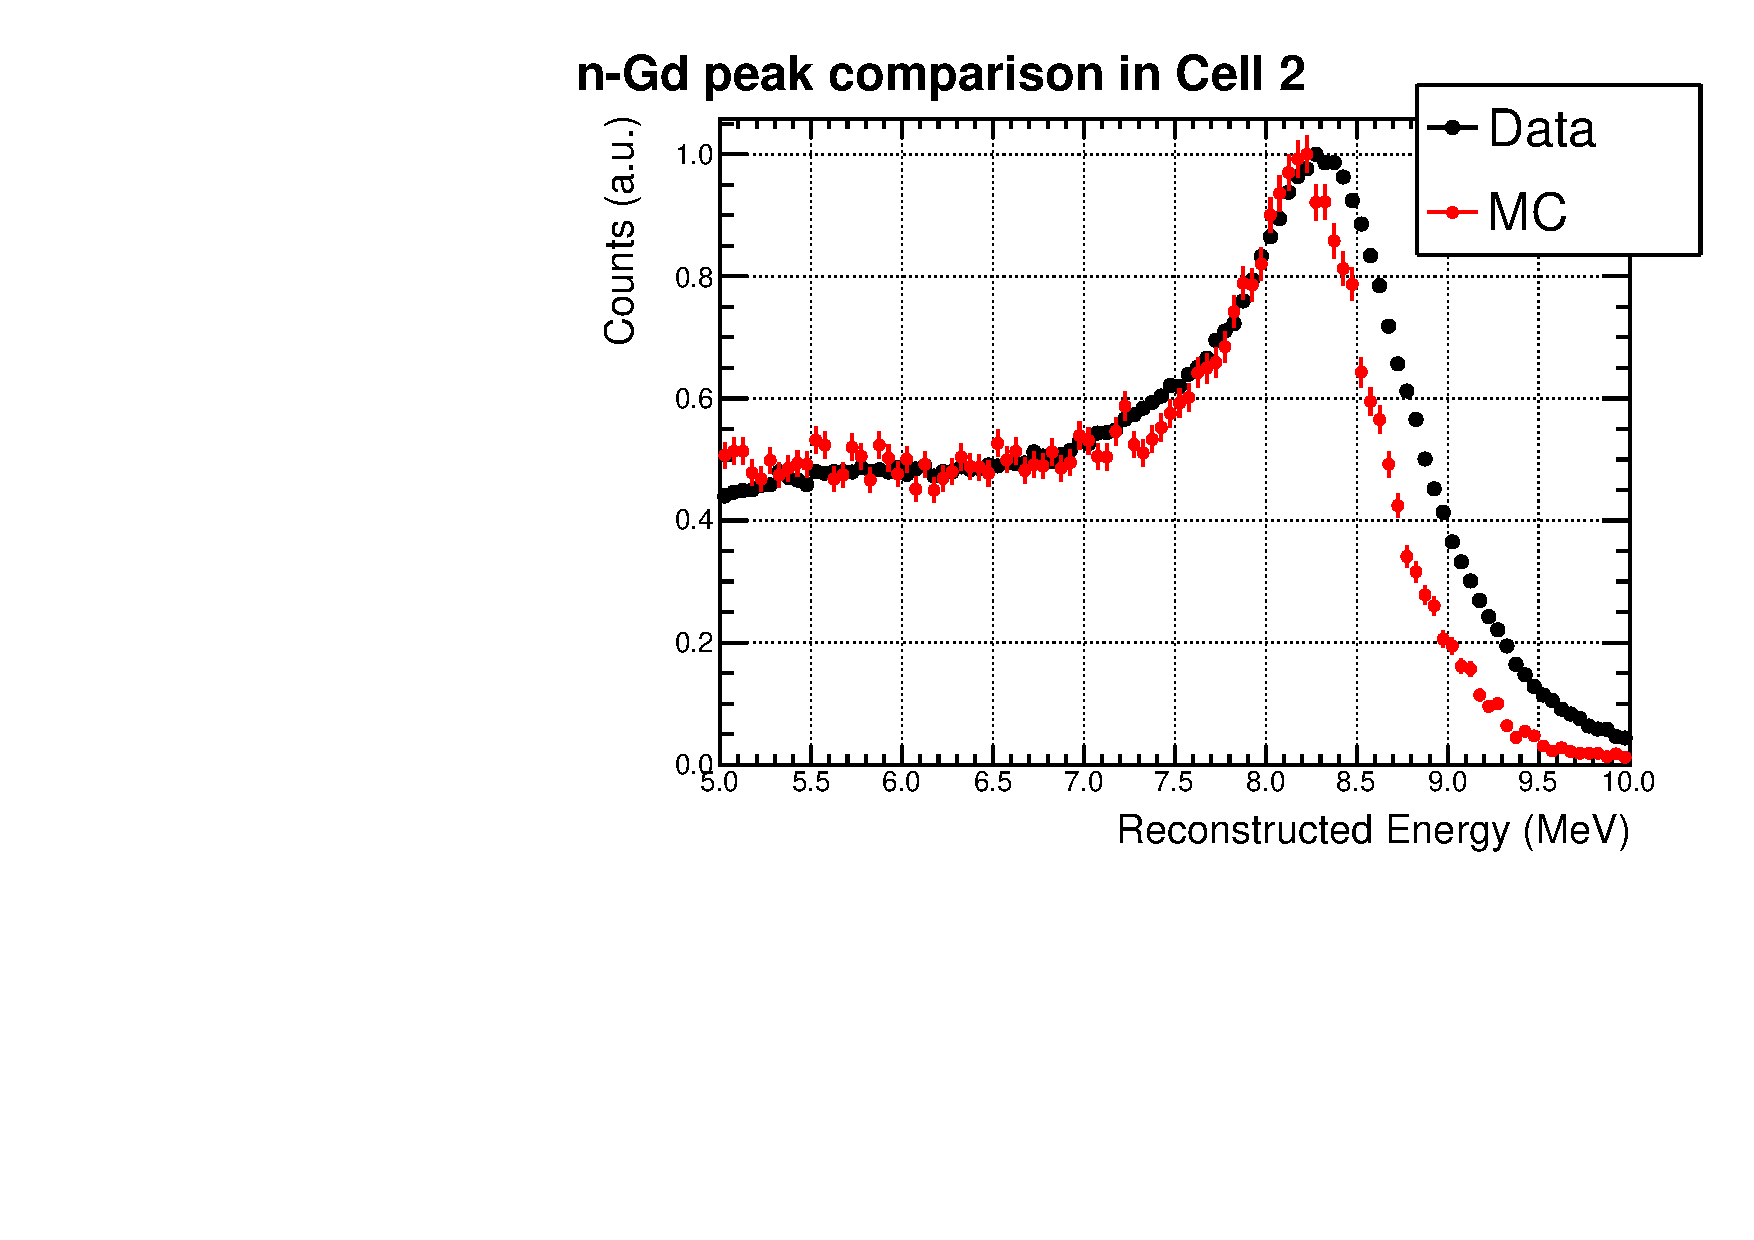
\includegraphics[width=1\textwidth]{images/Data_MC_peak_comparison_Cell2_Erec34_nGd_phase-2_fit-crystalball_stacks-20_analysis.pdf}
\caption{}
\label{fig:Data_MC_peak_comparison_Cell2_Erec34_nGd_phase-2_fit-crystalball_stacks-20_analysis.pdf}
\end{subfigure}


\caption[Comparaison de la forme des spectres de capture neutron entre les données et la simulation]{Comparaison de la forme des spectres de capture neutron entre les données et la simulation. (a) montre la distribution en énergie du n-H obtenu dans le MC par rapport aux données et (b) illustre les résultats du pic n-Gd. Seuls les événements identifiés dans la cellule 2 sont considérés sur ces deux graphs. Bien que l'intensité des événements à droite et à gauche des pics soit bien décrite par le MC, la largeur des pics est plus grande dans les données.}
\label{fig:comparison_nX_MC_Data_peaks_shape}

\end{figure}

}

La résolution des pics n-H et n-Gd est suivie en mesurant le paramètre $\sigma$, largeur de la gaussienne formant la partie droite du modèle Crystal-Ball. En phase 1, la résolution de chaque cellule reste stable sur toute la période: $\sim \SI{5.5}{\%}$. La cellule 4 a cependant une résolution plus haute à cause du découplage optique: $\sim \SI{6.5}{\%}$. L'évolution de la largeur des pics en phase 2 est présentée sur la figure \ref{fig:nX_resolution_evol} où on remarque que les cellules 1 et 6 ont une résolution sensiblement moins bonne que les autres cellules. Ce phénomène est probablement dû à leur proximité avec le Gamma-Catcher. En effet, les fuites de lumière $L_{1 \rightarrow 0}$ et $L_{6 \rightarrow 7}$ sont importantes, donc une partie de la lumière qui s'échappe vers les cellules 0 ou 7 peut être absorbée sur les bords du détecteur. Par ailleurs, une lente augmentation de la largeur des pics est notable. Celle-ci est régulière et commune à toutes les cellules. De nouveau, cet effet pointerait vers une lente dégradation des propriétés optiques du liquide scintillateur.\\

\subsection{Comparaison des pics de capture avec la simulation}

Dans le but de tester les non-linéarités de l'échelle en énergie et les effets de volume, les pics des gammas de capture ont également été mesurés dans le MC. Les neutrons cosmogéniques sont simulés (cf. Section \ref{sec:sim_gamma_from_nX}) et les coupures topologiques associées aux événements retardés sont appliquées. Une fonction Crystal Ball est ajustée sur les spectres afin de récupérer les valeurs de $\mu$ et $\sigma$ avec la même procédure que dans les données. Deux exemples de comparaison de spectres de captures neutroniques sont exposés sur la figure \ref{fig:comparison_nX_MC_Data_peaks_shape}. Bien que l'intensité des événements à droite et à gauche des pics soit correctement reproduite par le MC, les données ont une largeur $\sigma$ plus importante.\\

\afterpage{

\begin{figure}[h!]
\centering

\begin{subfigure}[b]{0.49\textwidth}
\centering
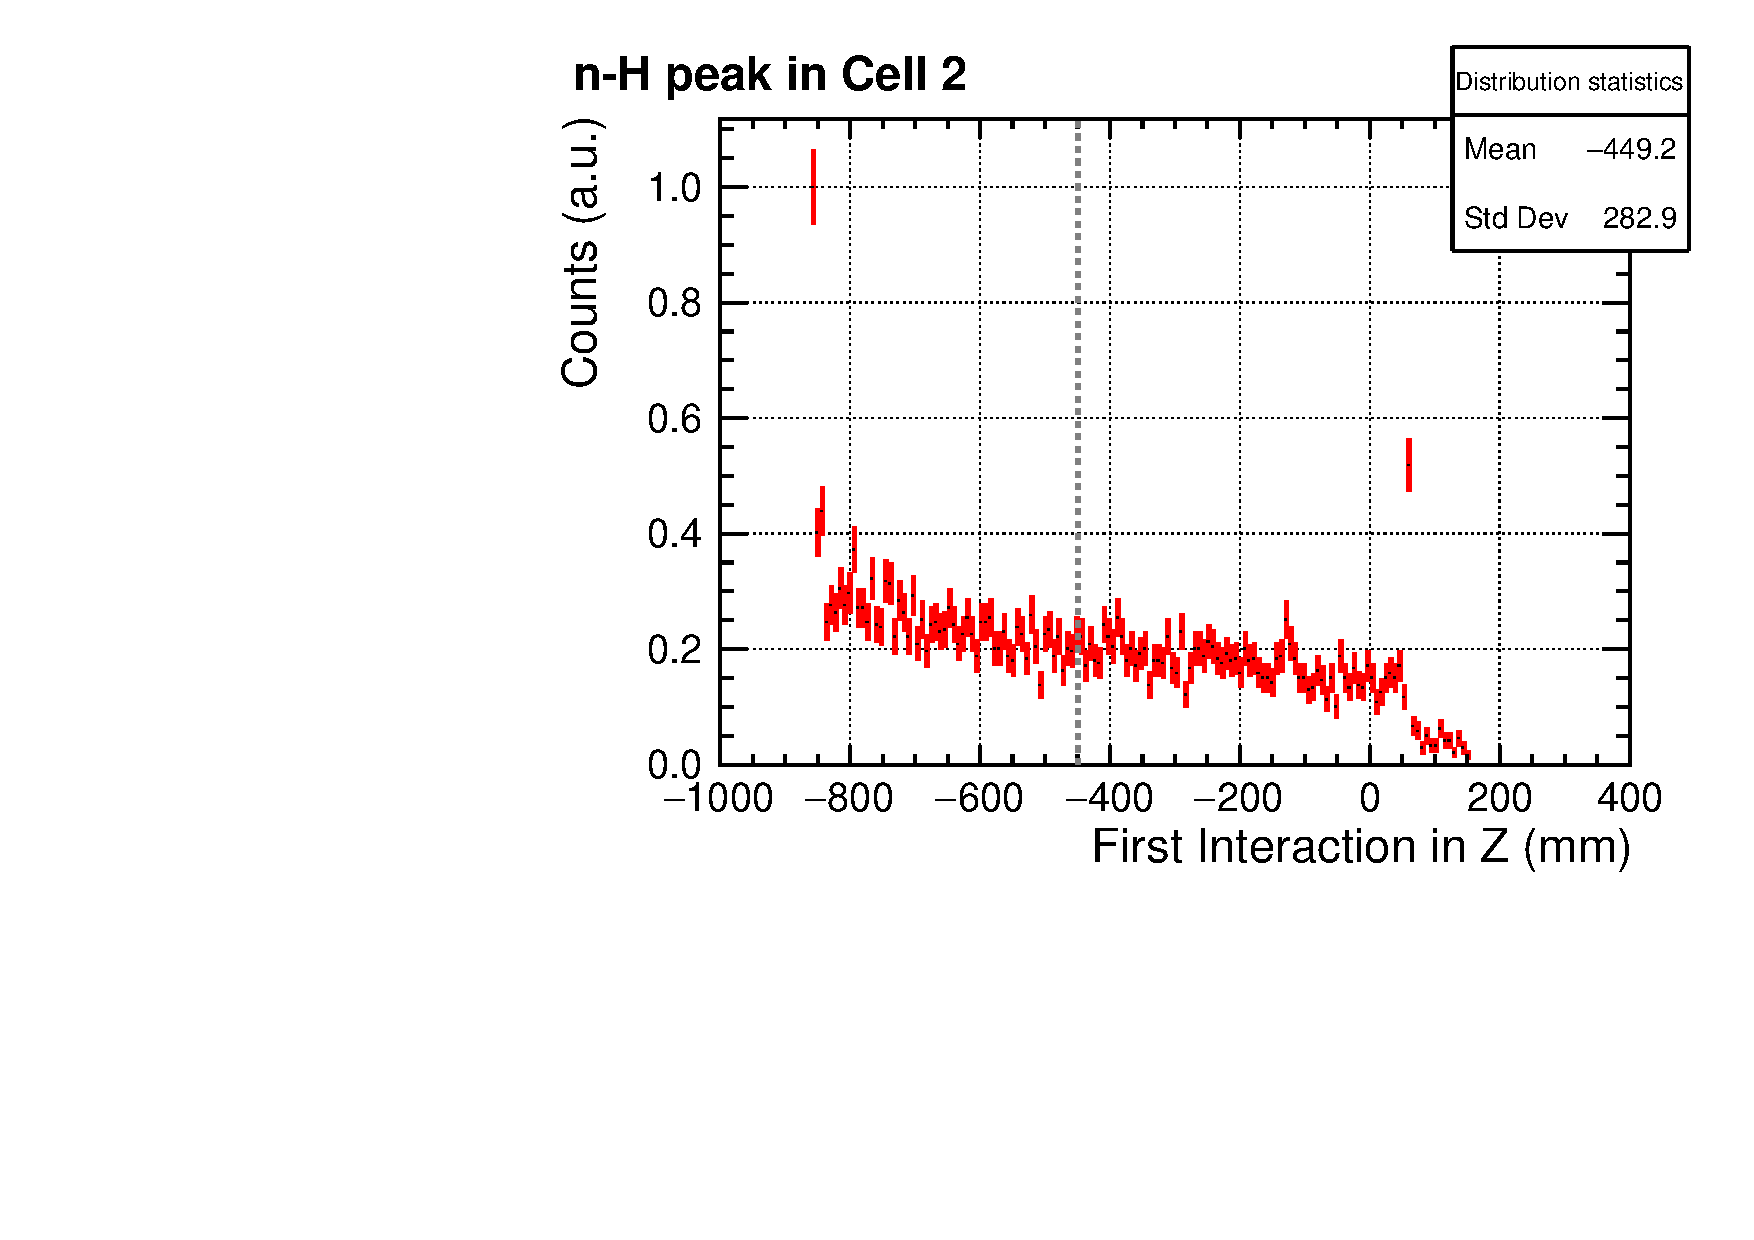
\includegraphics[width=1\textwidth]{images/nX_Z_example.pdf}
\caption{}
\label{fig:nX_Z_example.pdf}
\end{subfigure}
~ % attention ! space sensitive
\begin{subfigure}[b]{0.49\textwidth}
\centering
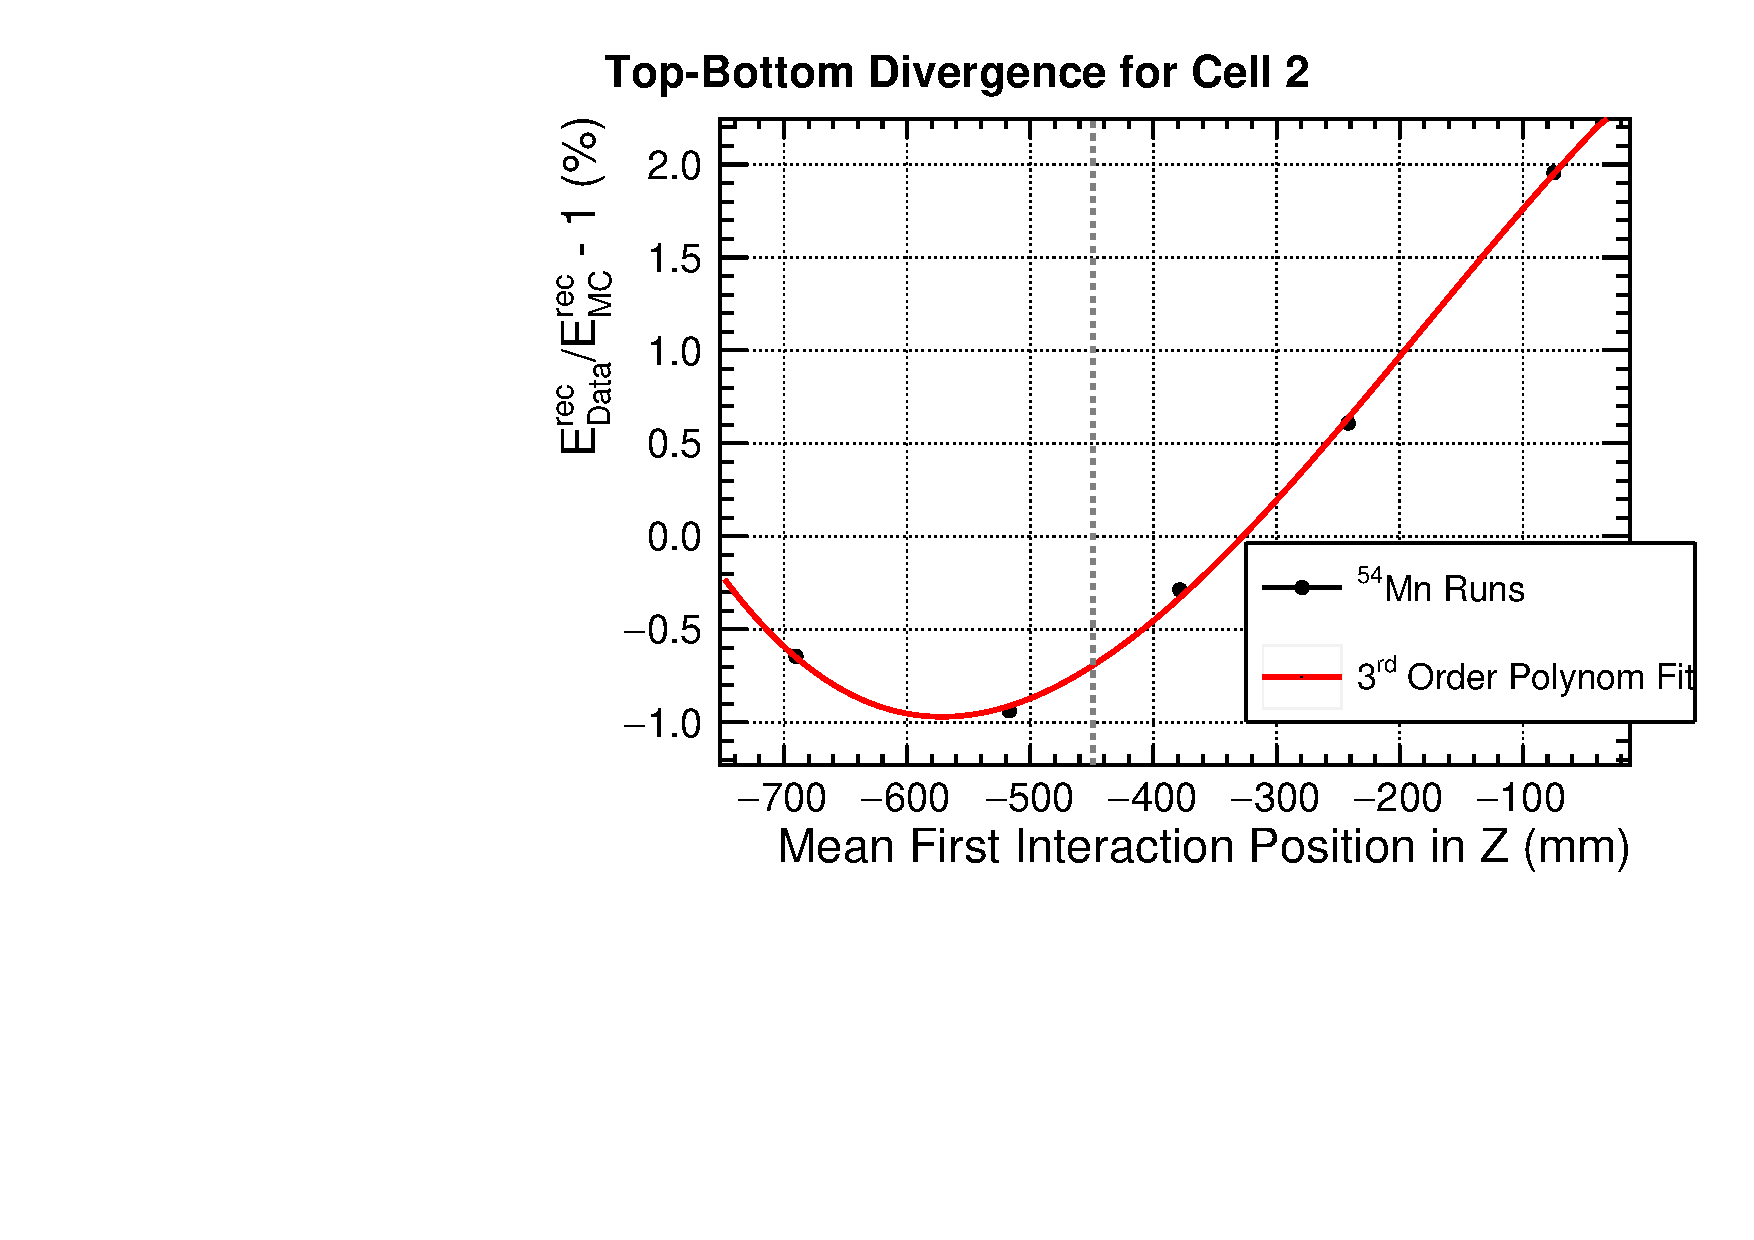
\includegraphics[width=1\textwidth]{images/Mn_Z_example.pdf}
\caption{}
\label{fig:Mn_Z_example.pdf}
\end{subfigure}


\caption[Estimation du biais induit par les inhomogénéités en Z du pic n-H]{Estimation du biais induit par les inhomogénéités en Z du pic n-H. La valeur moyenne de la première interaction en Z des événements n-H est déduite de (a), et cette valeur est reportée sur le modèle de dépendance de la réponse en énergie en fonction de Z (b). L'intersection entre la valeur de Z moyenne pour le n-H (ligne en pointillé grise) et le modèle (courbe rouge) donne la valeur du biais à corriger pour comparer la position du pic n-H avec les données. La cellule 2 a été choisie pour illustrer la méthode.}
\label{fig:nX_correction_bias_Z_with_Mn}

\end{figure}

\begin{figure}[h!]
  \centering
  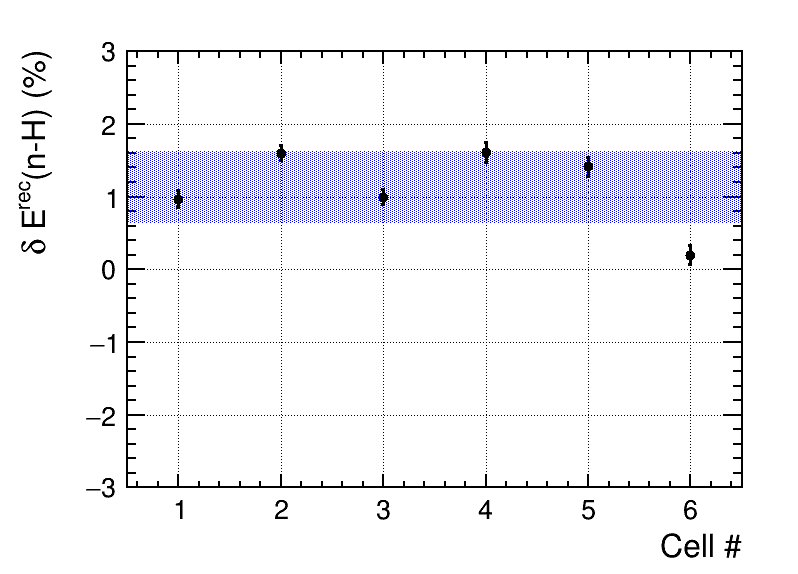
\includegraphics[width=0.75\linewidth]{images/DataMC_diff_Mn_nH_v34.png}
  \caption[Comparaison absolue entre la valeur du pic n-H dans les données et la simulation]{Comparaison absolue entre la valeur du pic n-H dans les données et la simulation. Chaque point a été corrigé du biais provoqué par l'asymétrie des dépôts d'énergie en Z des événements n-H. À titre indicatif, la bande bleue couvre une région de $\pm 0.5 \%$ autour de la moyenne des 6 cellules. Figure réalisée avec la version de calibration 34.}
  \label{fig:DataMC_diff_Mn_nH_v34.png}
\end{figure}

}

Pour comparer rigoureusement la position absolue des pics de capture, il est important de remarquer que la distribution des dépôts d'énergie des gammas de capture n-H est légèrement décentrée en Z (cf. Section \ref{sec:sim_gamma_from_nX}). Or, les coefficients de calibration utilisés dans cette analyse ont été ajustés en fusionnant des runs de $\ce{^{54}Mn}$ à 5 hauteurs, donc ont de fait une répartition des dépôts en énergie homogène en Z (cf. figure \ref{fig:mn_Edep_vertices}). Puisque la procédure de reconstruction en énergie ne corrige pas l'asymétrie de collection de lumière haut-bas, la différence de réponse pour des vertex décentrés en Z se répercute sur toute l'échelle en énergie. En estimant la moyenne en Z des dépôts d'énergie des gammas de capture, il est possible de corriger ce biais avec les runs $\ce{^{54}Mn}$. Pour ce faire, un modèle d'évolution de la divergence données-simulation en fonction de la hauteur est construit. Les runs $\ce{^{54}Mn}$ sont regroupés suivant leur hauteur en Z, et les coupures topologiques de la calibration (cf. Section \ref{sec:cuts_for_Erec_tuning}) sont sollicitées. Pour chaque cellule et chaque Z, la position moyenne des dépôts d'énergie en Z est mesurée et la valeur la plus probable de l'énergie reconstruite est extraite avec un fit local gaussien dans les données et la simulation. L'écart des valeurs des pics entre données et simulation est tracé en fonction de Z et un modèle polynomial du 3e ordre est ajusté: voire figure \ref{fig:nX_correction_bias_Z_with_Mn}. En reportant la valeur moyenne en Z des événements n-H sur la courbe ajustée, la valeur du biais est déduite. La procédure est répétée pour chaque cellule et les écarts en énergie reconstruite des pics n-H sont corrigés:

\begin{equation}
    \delta E^\textrm{rec} (\textrm{n-H}) = \frac{E^\textrm{rec}_\textrm{Data} (\textrm{n-H}) - E^\textrm{rec}_\textrm{MC} (\textrm{n-H})}{E^\textrm{rec}_\textrm{MC} (\textrm{n-H})} - \delta E^\textrm{rec} (\ce{^{54}Mn}, Z).
\end{equation}

\bigbreak

La distribution des $\delta E^\textrm{rec} (\textrm{n-H})$ est présenté sur la figure \ref{fig:DataMC_diff_Mn_nH_v34.png}. Excepté la cellule 6, toutes les cellules ont un décalage positif entre 1 et 1.5 \%. Le fait que les données n-H soient reconstruites avec une moyenne plus haute que la simulation était déjà visible sur la figure \ref{fig:comparison_nX_MC_Data_peaks_shape}. Visuellement l'accord apparaît très bon sur toute la partie gauche des spectres et le décalage de la valeur moyenne semble provenir d'un manque de largeur à droite des spectres simulés.\\

Cette constatation nous a naturellement ramenés à la principale imperfection du MC, constatée figure \ref{fig:FivePositionsComparison_cell6} : l'amplitude des effets haut-bas dans le MC est inférieure à celle des données. Des études en cours montrent que ce désaccord peut être corrigé par l'introduction d'une faible valeur d'absorption de la lumière dans les parois réfléchissantes, jusqu'à présent absent de la simulation. Deux justifications physiques d'un tel terme ont été identifiées :

\begin{itemize}[label=\textbullet]
    \item Le revêtement Téflon des tubes de calibration, défini comme blanc dans la simulation, est en réalité gris (cf. figure \ref{fig:photo_calib_tube_Teflon.jpg}).
    \item Lorsqu'une fraction de la lumière est transmise dans la cellule voisine à travers l'ESR (angle d'incidence supérieur à l'angle critique et gap d'air rempli de liquide scintillateur) une partie de cette lumière doit être absorbée par le filet en nylon positionné derrière le film réfléchissant (cf. figure \ref{fig:20140619_161654.jpg}).
\end{itemize}

\bigbreak

Il a été montré que l'abaissement de 20 \% de la réflectivité des tubes de calibration et 4 \% d'absorption de la lumière transmise à travers l'ESR permettent de retrouver un très bon accord sur les largeurs des distributions données et MC des pics de capture neutron. L'accord sur les valeurs moyennes demande un \textit{reprocessing} complet de toute la procédure de calibration, en cours au moment de la rédaction de cette thèse.

\bigbreak

%La raison pour laquelle les résultats de l'analyse du quenching (cf. \ref{fig:DataMC_ErecDet_v34_meanZ_allCells.pdf}) n'ont pas mesuré une telle déviation pourrait se trouver dans le fait que les distributions des dépôts d'énergie des runs de calibration sont centrés autour du tube en X et Y. En effet, la taille des cellules en Y n'est pas négligeable devant l'extension spatiale des dépôts d'énergie des sources placées dans le tube central:

%\begin{equation}
%    \Delta Y_\textrm{cell}/2 \simeq \SI{45}{cm} > \Delta L_\gamma,
%\end{equation}

\afterpage{

\begin{figure}[h!]
\centering

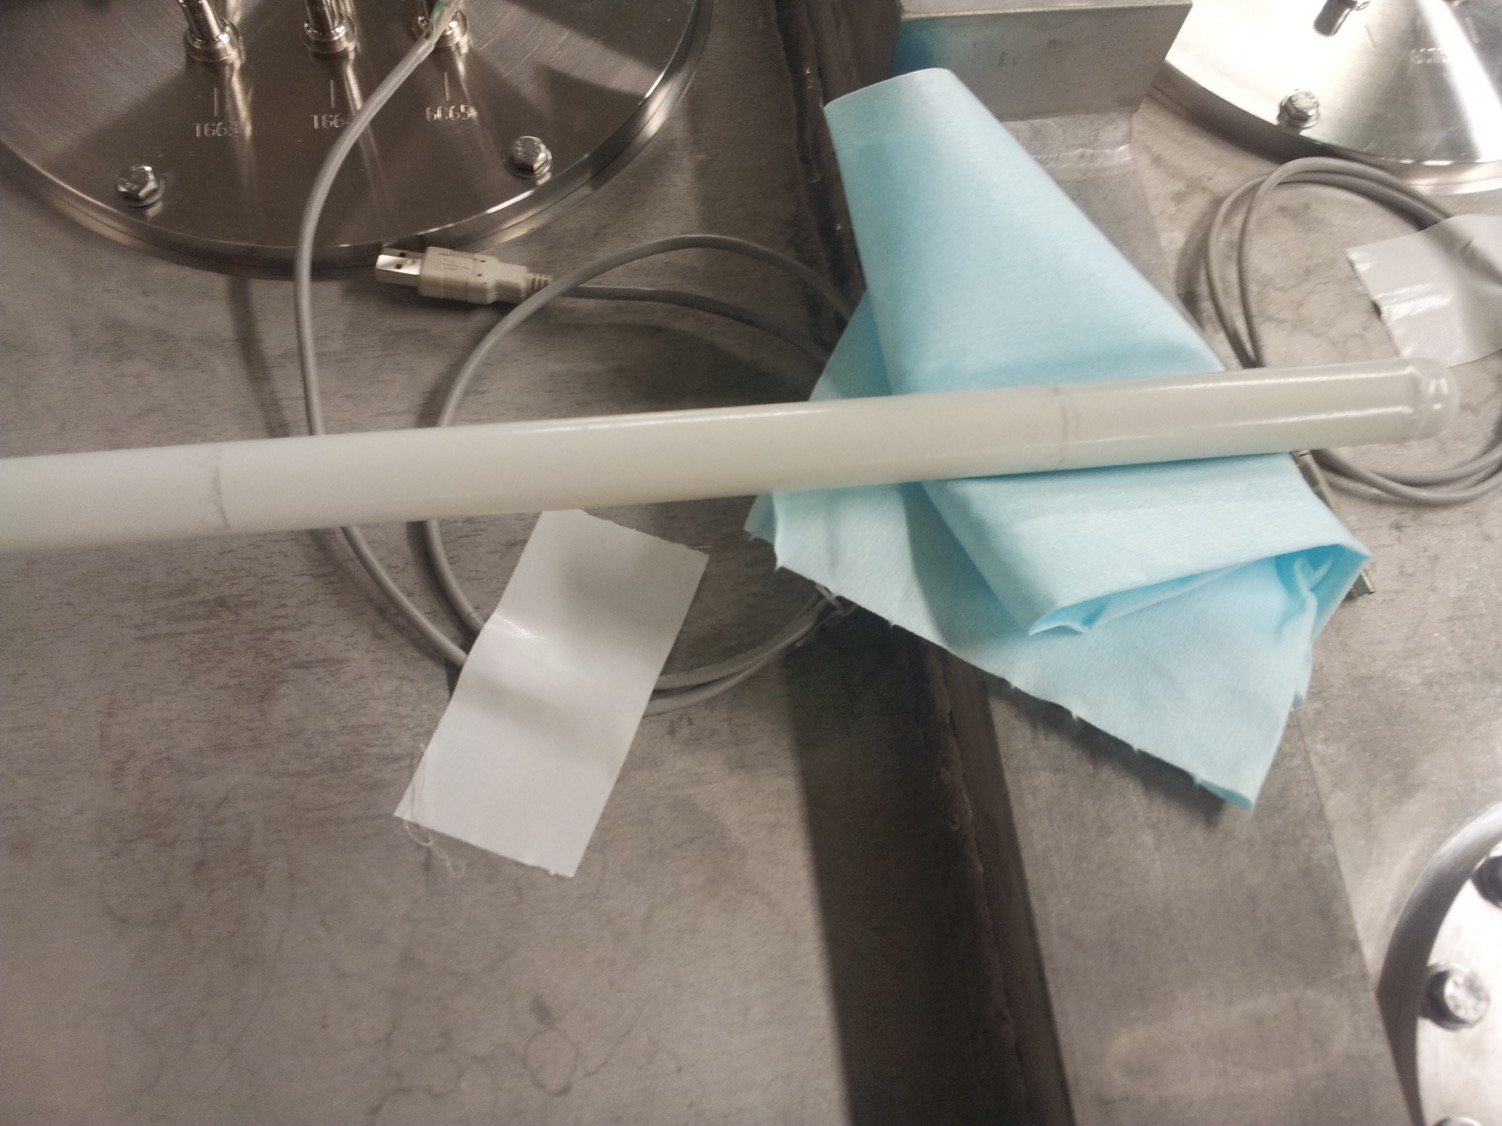
\includegraphics[width=0.8\textwidth]{images/photo_calib_tube_Teflon.jpg}
\caption[Photo du tube de calibration en Téflon]{Photo du tube de calibration en Téflon. Les tubes de calibrations sont de couleur grise alors que dans la simulation ils ont été considérés blancs. Cette inexactitude serait responsable du désaccord du pic n-H entre les données et le MC.}
\label{fig:photo_calib_tube_Teflon.jpg}

%

%\begin{subfigure}[b]{0.49\textwidth}
%\centering
%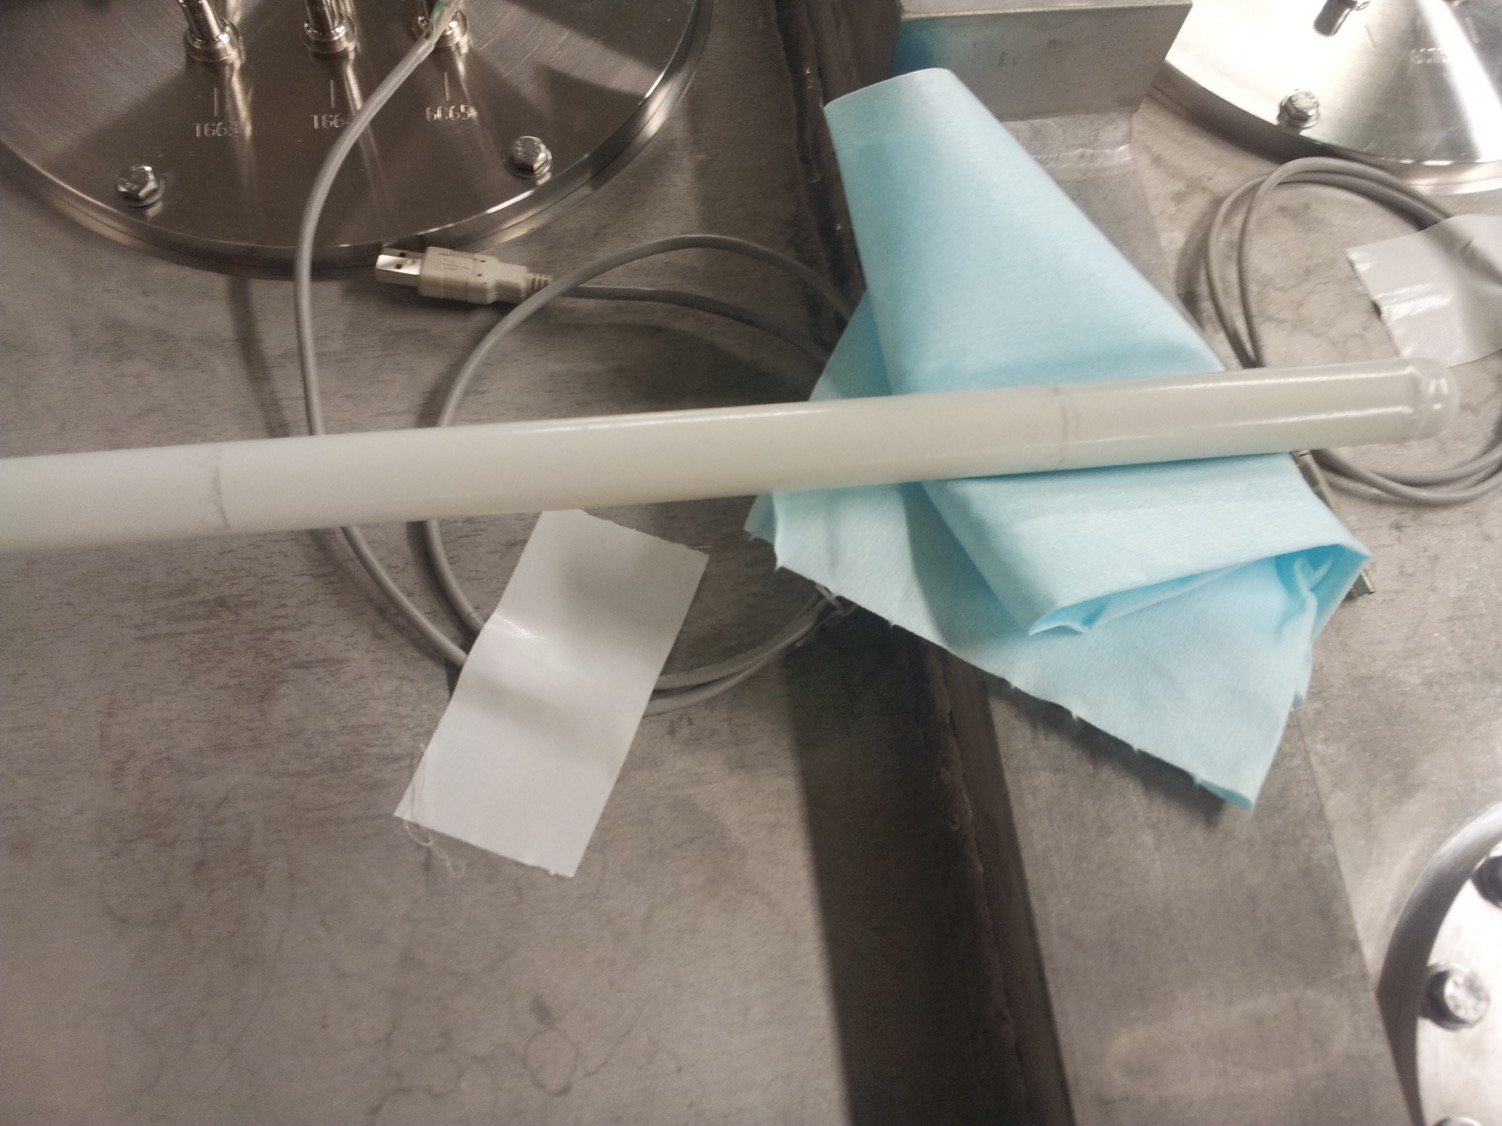
\includegraphics[width=1\textwidth]{images/photo_calib_tube_Teflon.jpg}
%\caption{}
%\label{fig:photo_calib_tube_Teflon.jpg}
%\end{subfigure}

%\begin{subfigure}[b]{0.49\textwidth}
%\centering
%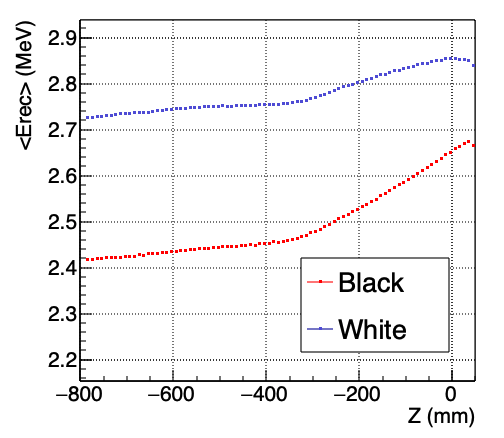
\includegraphics[width=1\textwidth]{images/bw_top_bottom.png}
%\caption{}
%\label{fig:bw_top_bottom.png}
%\end{subfigure}
%~ % attention ! space sensitive
%\begin{subfigure}[b]{0.49\textwidth}
%\centering
%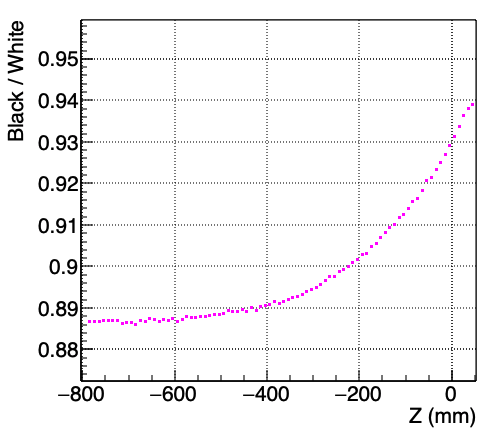
\includegraphics[width=1\textwidth]{images/bw_relative_top_bottom.png}
%\caption{}
%\label{fig:bw_relative_top_bottom.png}
%\end{subfigure}


%\caption[Effet de la couleur du tube de calibration dans la simulation]{Effet de la couleur du tube de calibration dans la simulation. Les tubes en Téflon dans le détecteur ne sont pas tout à fait blancs (a) bien qu'ils l'aient été considéré dans le MC. Le changement de la couleur des tubes affecte l'asymétrie de réponse haut-bas (b), et le rapport entre noir et blanc montre que les effets haut-bas peuvent varier sur un bras de levier de $\sim 6 \%$ (c). (source : \cite{docdb946})}
%\label{fig:black_or_white}

\end{figure}

\begin{figure}[h!]
\centering
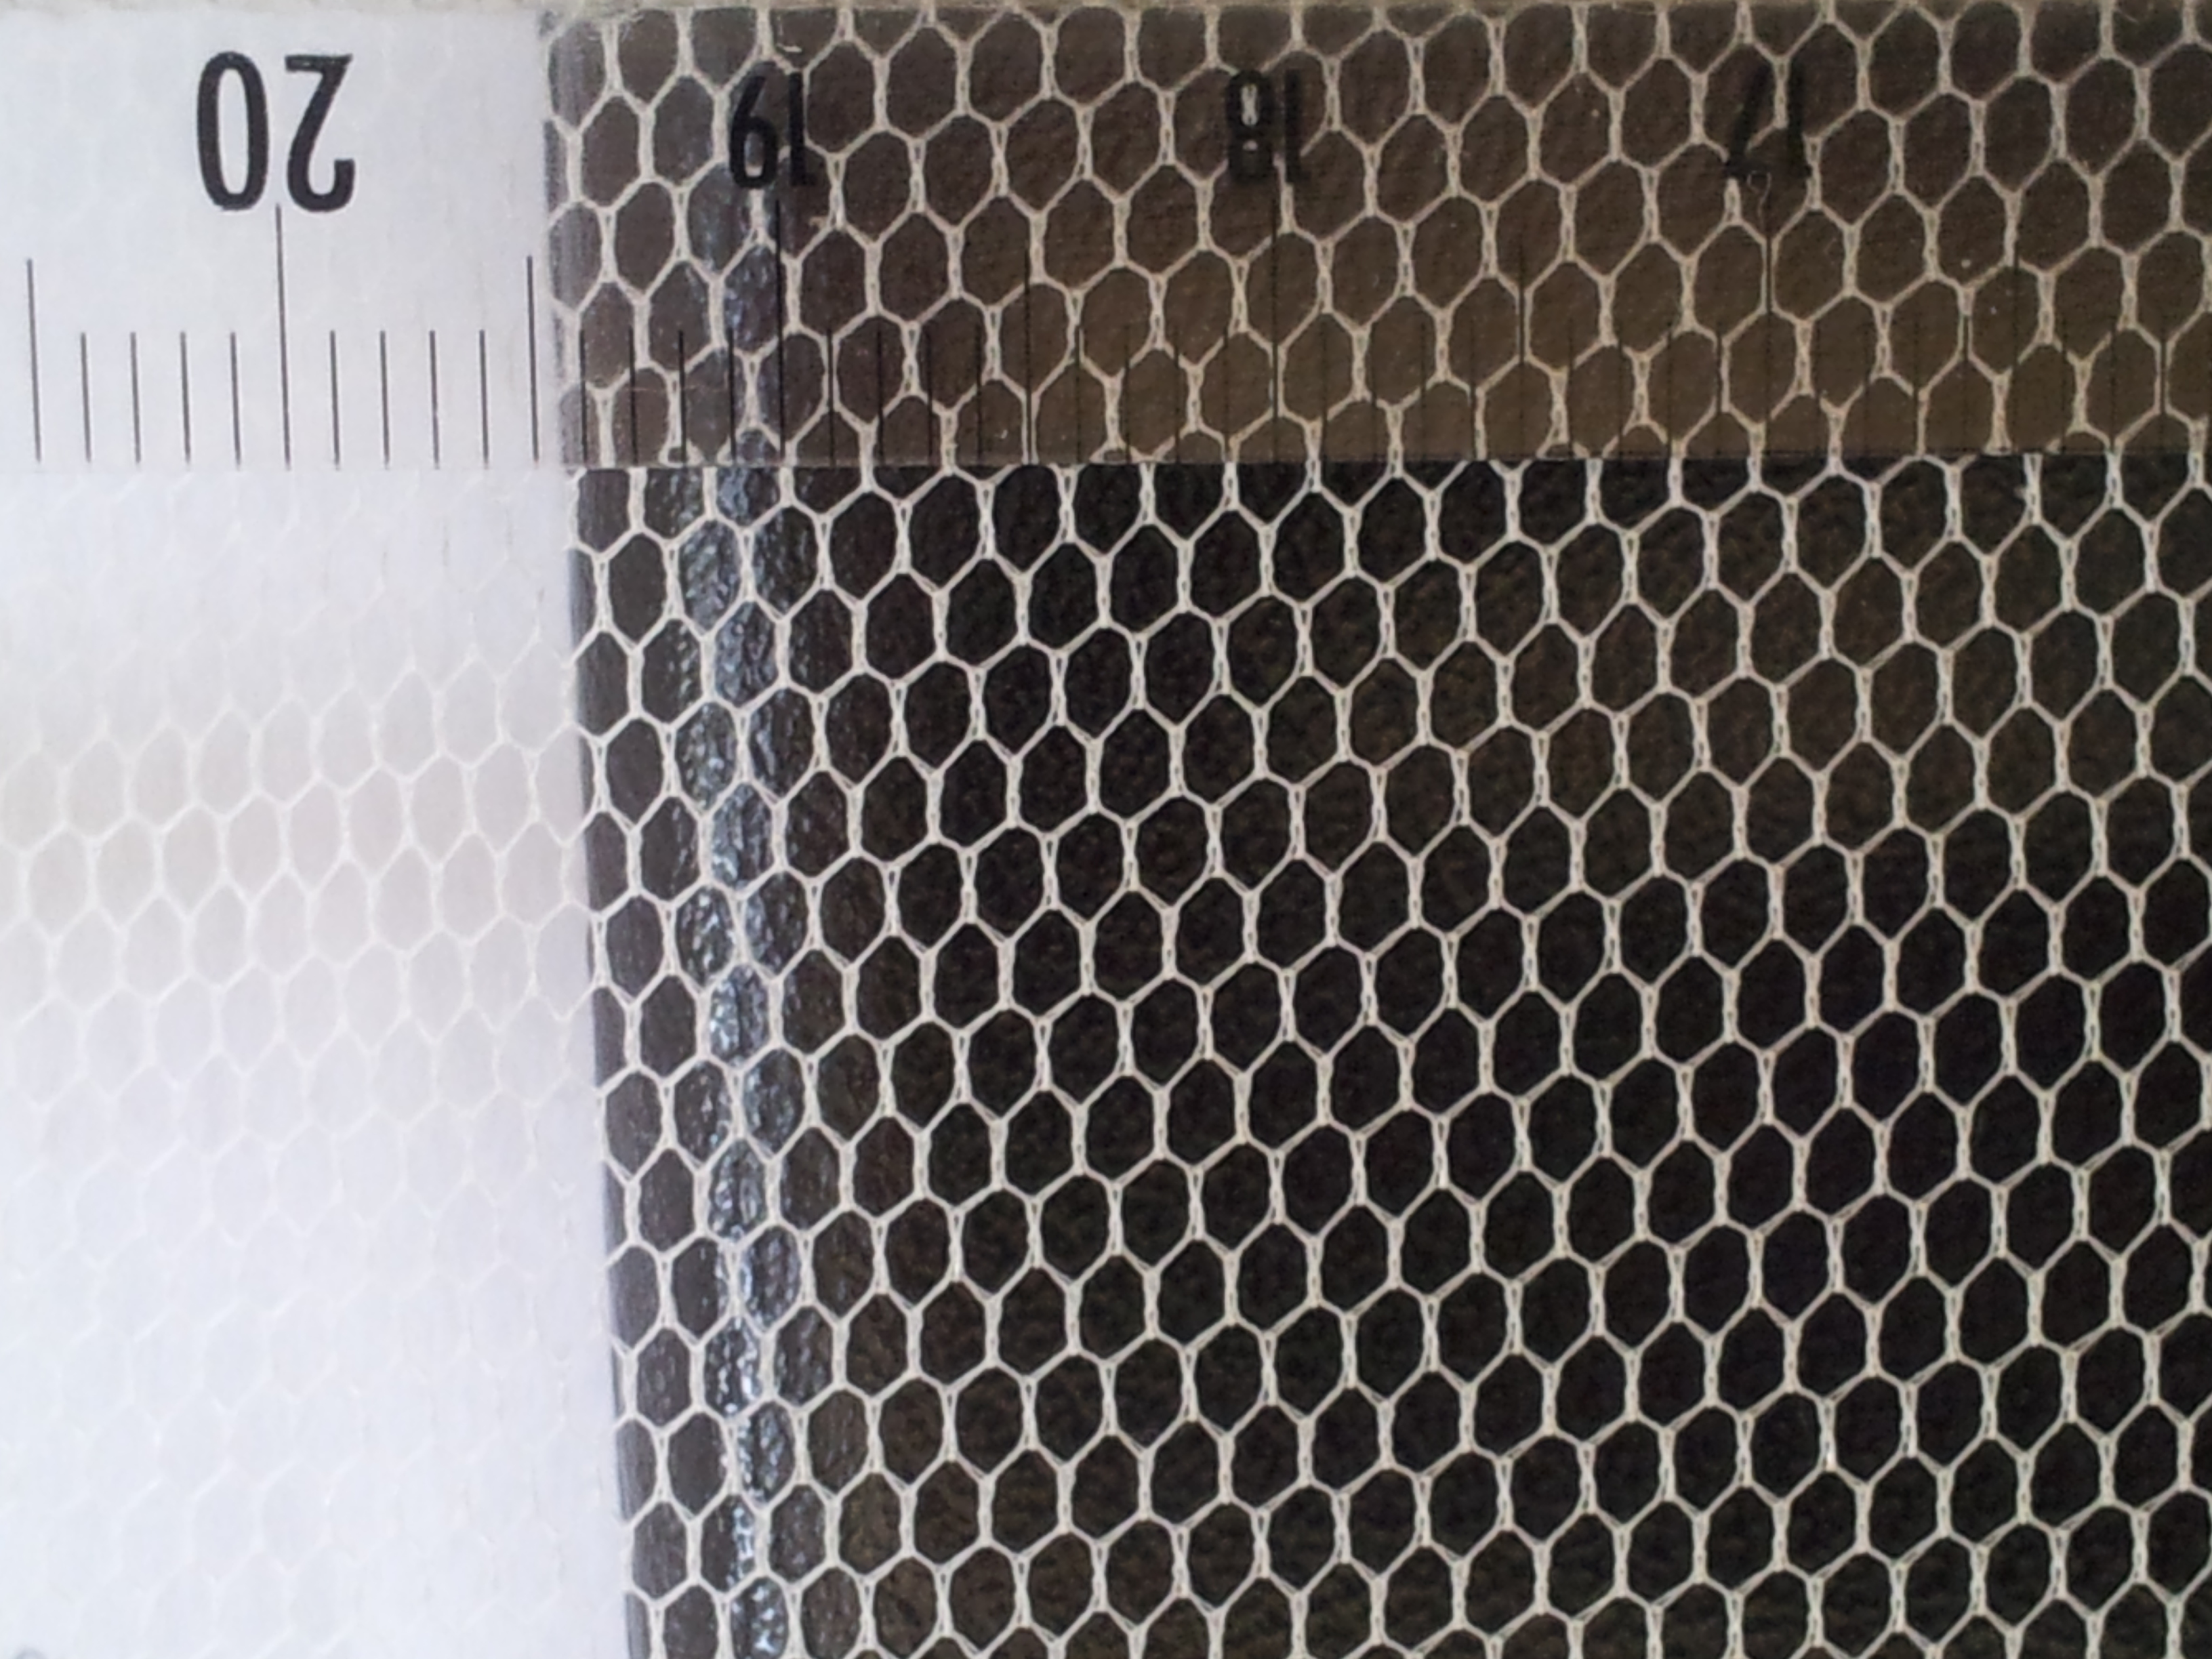
\includegraphics[width=0.8\textwidth]{images/20140619_161654.jpg}
\caption[Photo du voile en nylon intercalé entre les films réfléchissants]{Photo du voile en nylon intercalé entre les films réfléchissants. Le voile en nylon doit être responsable de l'absorption d'une partie de la lumière. Cet aspect a été négligé dans la simulation jusqu'alors.}
\label{fig:20140619_161654.jpg}
\end{figure}

\clearpage

}

%\bigbreak
%
%où $\Delta L_\gamma$ vaut typiquement $\SI{18}{cm}$ à $\SI{0.835}{MeV}$ contre $\SI{40}{cm}$ à $\SI{4.4}{MeV}$ \cite{docdb816}. L'échelle en énergie n'a donc pas été contrainte pour des vertex situés contre les parois qui séparent les longues cellules du Gamma-Catcher des cellules de la Target. Il serait intéressant de comparer la réponse en énergie données-MC en exploitant les runs de calibrations réalisées avec le pantographe à l'extérieur du détecteur (cf. Section \ref{sec:data_quality_control}). En appliquant des coupures strictes pour que les événements gammas d'étude n'aient interagi que dans les cellules de la Target, la distribution des dépôts d'énergie en Y sont opposée à celle des calibrations internes. La mesure de l'écart en énergie reconstruite entre la simulation et les données permettrait de délibérer sur la dépendance relative en Y de la collection de lumière.\\
%
%Si cette hypothèse est validée, il reste à comprendre la raison pour laquelle le MC n'a pas le même comportement sur les bords des cellules. Un des candidats suspectés invoque une mauvaise description de la couleur du tube de calibration. Les tubes en Téflon ont initialement été considérés comme \og blanc \fg{}, c'est-à-dire avec un facteur d'absorption nul, or les tubes de calibration dans \textsc{Stereo} ne le sont pas à 100 \% comme le montre la photo sur figure \ref{fig:photo_calib_tube_Teflon.jpg}. Pour mettre à l'épreuve cette hypothèse, des électrons répartis uniformément dans la Target ont été simulés avec soit un tube blanc, soit un tube noir.  Les différentes extensions spatiales des sources $\lambda_\gamma$ sont reproduites en pondérant chaque événement par sa distance au tube $d$ avec une exponentielle : $\textrm{exp}\left(-d/\lambda_\gamma\right)$. L'écart relatif entre blanc et noir laisse apparaitre un biais à hauteur de $\sim 0.7\%$ entre l'extension spatiale du $\ce{^{54}Mn}$ et le cas uniforme. Le bras de levier blanc-noir n'est néanmoins pas suffisant pour expliquer le décalage du pic n-H, d'autant que les données de quenching ne se montre pas d'accroissement du désaccord données-MC en fonction de l'énergie, et donc de l'extension spatiale en Y (cf. figure \ref{fig:DataMC_ErecDet_v34_meanZ_allCells.pdf}). En revanche la couleur des tubes affecte significativement l'effet haut-bas qui, dans la simulation, a été ajusté à l'aide de la longueur d'atténuation du liquide. Les Figures \ref{fig:bw_top_bottom.png} et \ref{fig:bw_relative_top_bottom.png} montrent que la différence d'asymétrie haut-bas sur la collection de lumière entre blanc et noir a une amplitude de $\sim 6 \%$. Or, la largeur des pics n-H dans \textsc{Stereo} est due à deux principaux facteurs: la photo-statistique ($\sim 4 \%$ à $\SI{2.2}{MeV}$) et l'effet haut-bas. La couleur des tubes est donc un candidat de choix pour expliquer la différence de largeur vue sur la figure \ref{fig:comparison_nX_MC_Data_peaks_shape}. Pour ce qui est de la position absolue des pics n-H, un nouvel ajustement de la longueur d'atténuation pourrait résoudre le désaccord.

%\afterpage{
%
%
%\begin{figure}[h!]
%  \centering
%  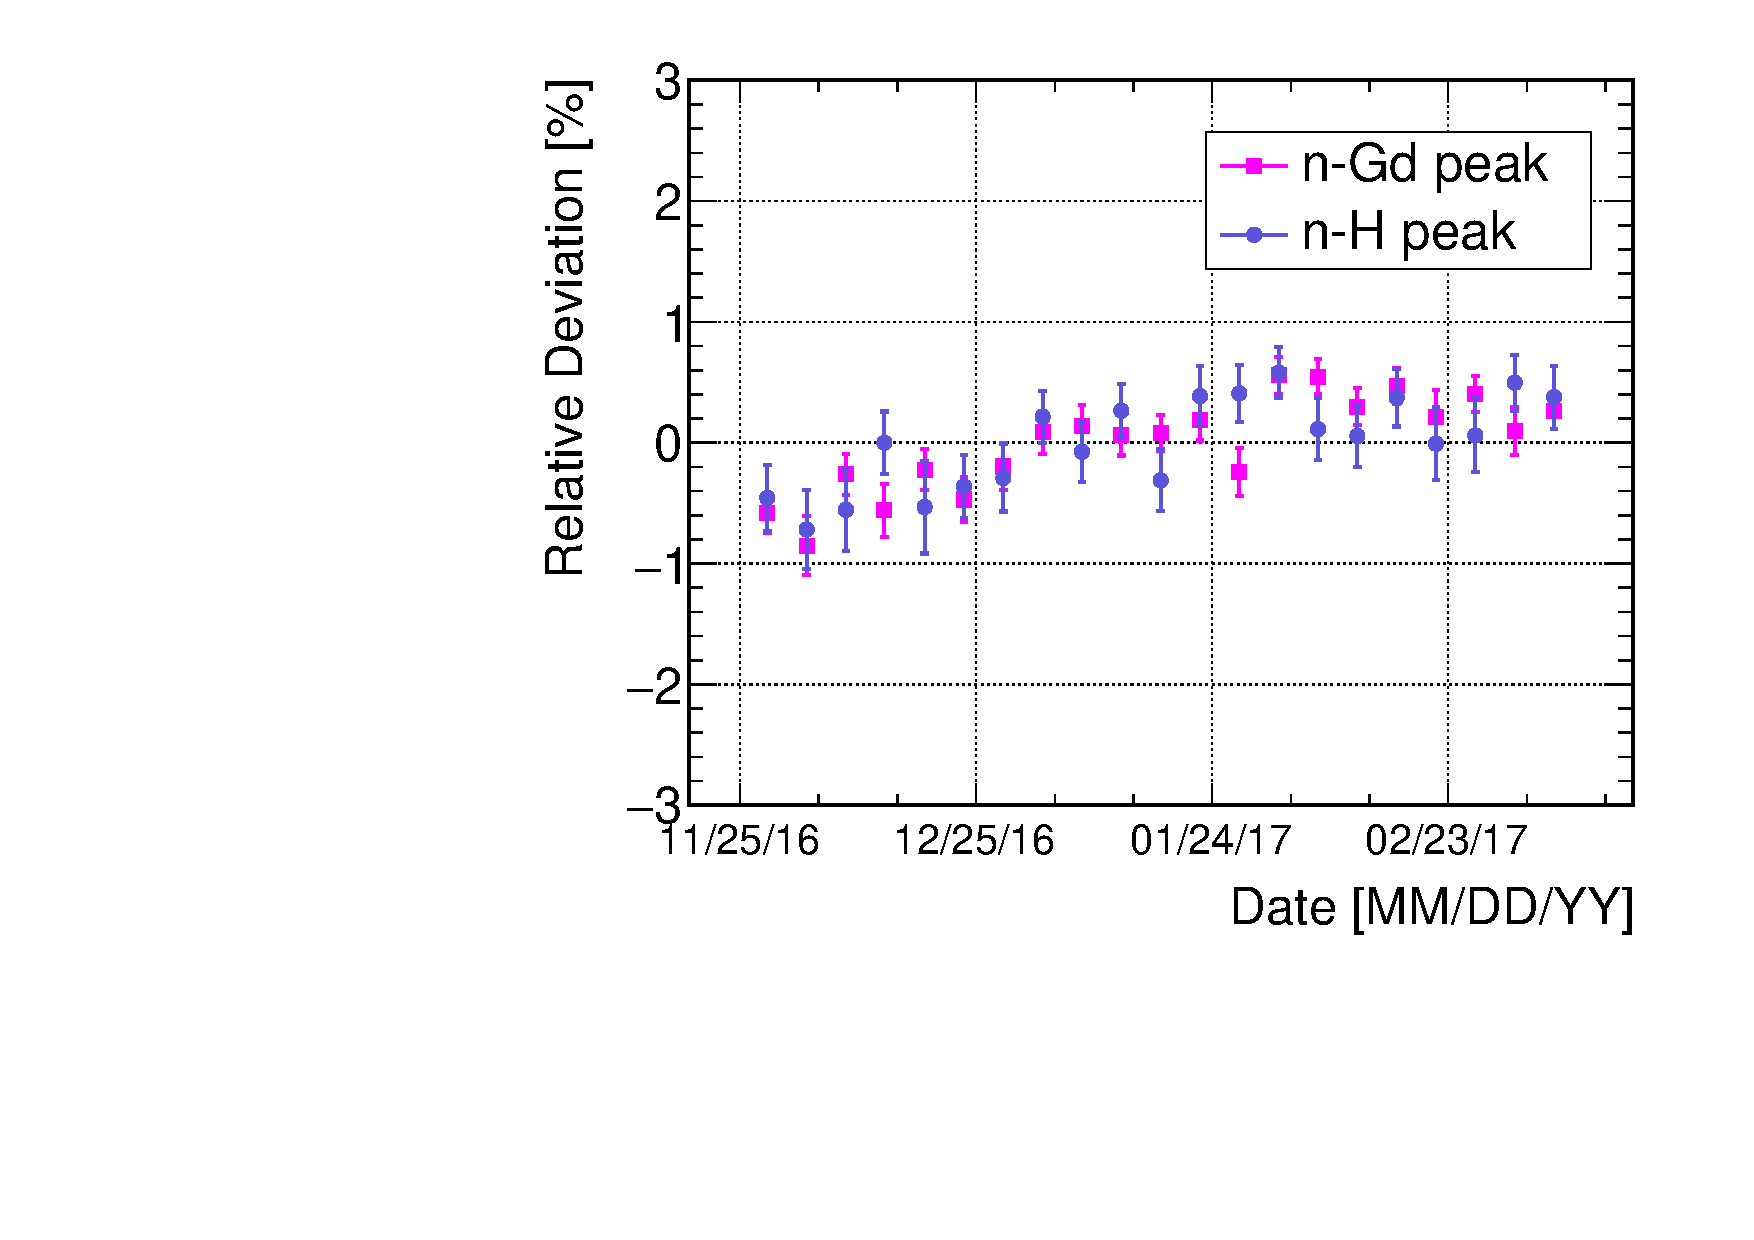
\includegraphics[width=0.8\linewidth]{images/nH-nGd_Time-stability_gauss.pdf}
%  \captionof{figure}{Déviations relatives de la valeur du pic d'énergie reconstruite des gamma de capture n-H et n-Gd pendant la phase 1.}
%  \label{fig:comparison_nH_nGd_p1}
%\end{figure}
%
%\clearpage
%}

% La cascade gamma du Gadolinium après capture neutron constitue aussi un moyen de sonder la réponse en énergie. En effet, la désexcitation du Gadolinium se fait en émettant simultanément plusieurs gammas d'environ $\SI{2}{MeV}$ dans différentes directions. Ces derniers déposent de l'énergie dans plusieurs cellules à la fois, nous offrant une situation inédite pour tester l'échelle en énergie.\\

% Contrairement au pic n-H, l'étude de la cascade n-Gd n'est pas directement comparée avec la simulation dans cette étude. La complexité de la décroissante du noyau de Gadolinium nous empêche de comparer la position du pic en énergie dans la simulation avec une précision satisfaisante. De plus, la comparaison données-simulation du pic n-Gd a déjà été effectuée avec la source d'AmBe (voire Section ). L'objet de cette étude est de comparer l'évolution dans le temps du pic n-Gd à celle du pic n-H.\\

%Comme pour l'étude de la capture sur Hydrogène, les données sont triées par période et par cellule. La valeur du pic n-Gd est obtenue en ajustant localement une fonction \og Crystal Ball \fg{}. Un exemple de fit est présenté sur le Figure . La figure \ref{fig:comparison_nH_nGd_p1} montre une correlation significative entre le pic n-H et n-Gd. On attribuera l'évolution résiduelle de l'énergie reconstruite à un changement asymétrique de réflectivité des parois des cellules. Un candidat potentiel pour expliquer cet effet serait la lente dégradation de la plaque du fond de la cuve.\\

\subsection{Mesures du spectre de la décroissance beta du bore 12}

Le spectre de décroissance beta du bore 12 permet de poser des contraintes sur le comportement de la reconstruction en énergie jusqu'à plus de $\SI{12}{MeV}$. La production du bore 12 est d'origine cosmique. Les muons qui atteignent le détecteur peuvent induire la production de cet élément par deux canaux principalement. Les muons de basse énergie ($< \SI{120}{MeV}$) s'arrêtent parfois dans le détecteur interne, et se font capturer par un atome de Carbone 12 où ils descendent jusqu'à l'orbitale 1S (1\% des cas) \cite{Reynolds:1963zz}. Le fort recouvrement de cette orbitale avec le noyau favorise les courants chargés avec un proton et donc la formation de $\ce{^{12}B}$. Le deuxième canal de production du bore 12 passe par la spallation des noyaux par des muons de hautes énergies ($> \SI{200}{MeV}$). La spallation produit des neutrons qui peuvent à leur tour transformer les noyaux de Carbon 12 en bore 12 via la réaction (n-p).\\

Le bore 12 est un noyau instable qui a une durée de vie moyenne de $\tau (\ce{^{12}B}) \simeq \SI{20}{ms}$. Il décroit par réaction beta en émettant un électron dont le spectre en énergie s'étale jusque $\SI{13.4}{MeV}$. L'extraction du spectre beta est effectuée en identifiant des paires d'événements contenant un muon dans la fenêtre Prompt et l'électron de décroissance beta dans la fenêtre Retardée. Les conditions d'isolation des paires ont été relâchées (celles-ci sont définies dans la Section \ref{sec:time_cuts_pair_search}), car le taux de muons est trop élevé : environ 20 $\mu^{\pm}$ sont attendus par unité de $\tau (\ce{^{12}B})$.\\

\afterpage{

\begin{figure}[h!]
  \centering
  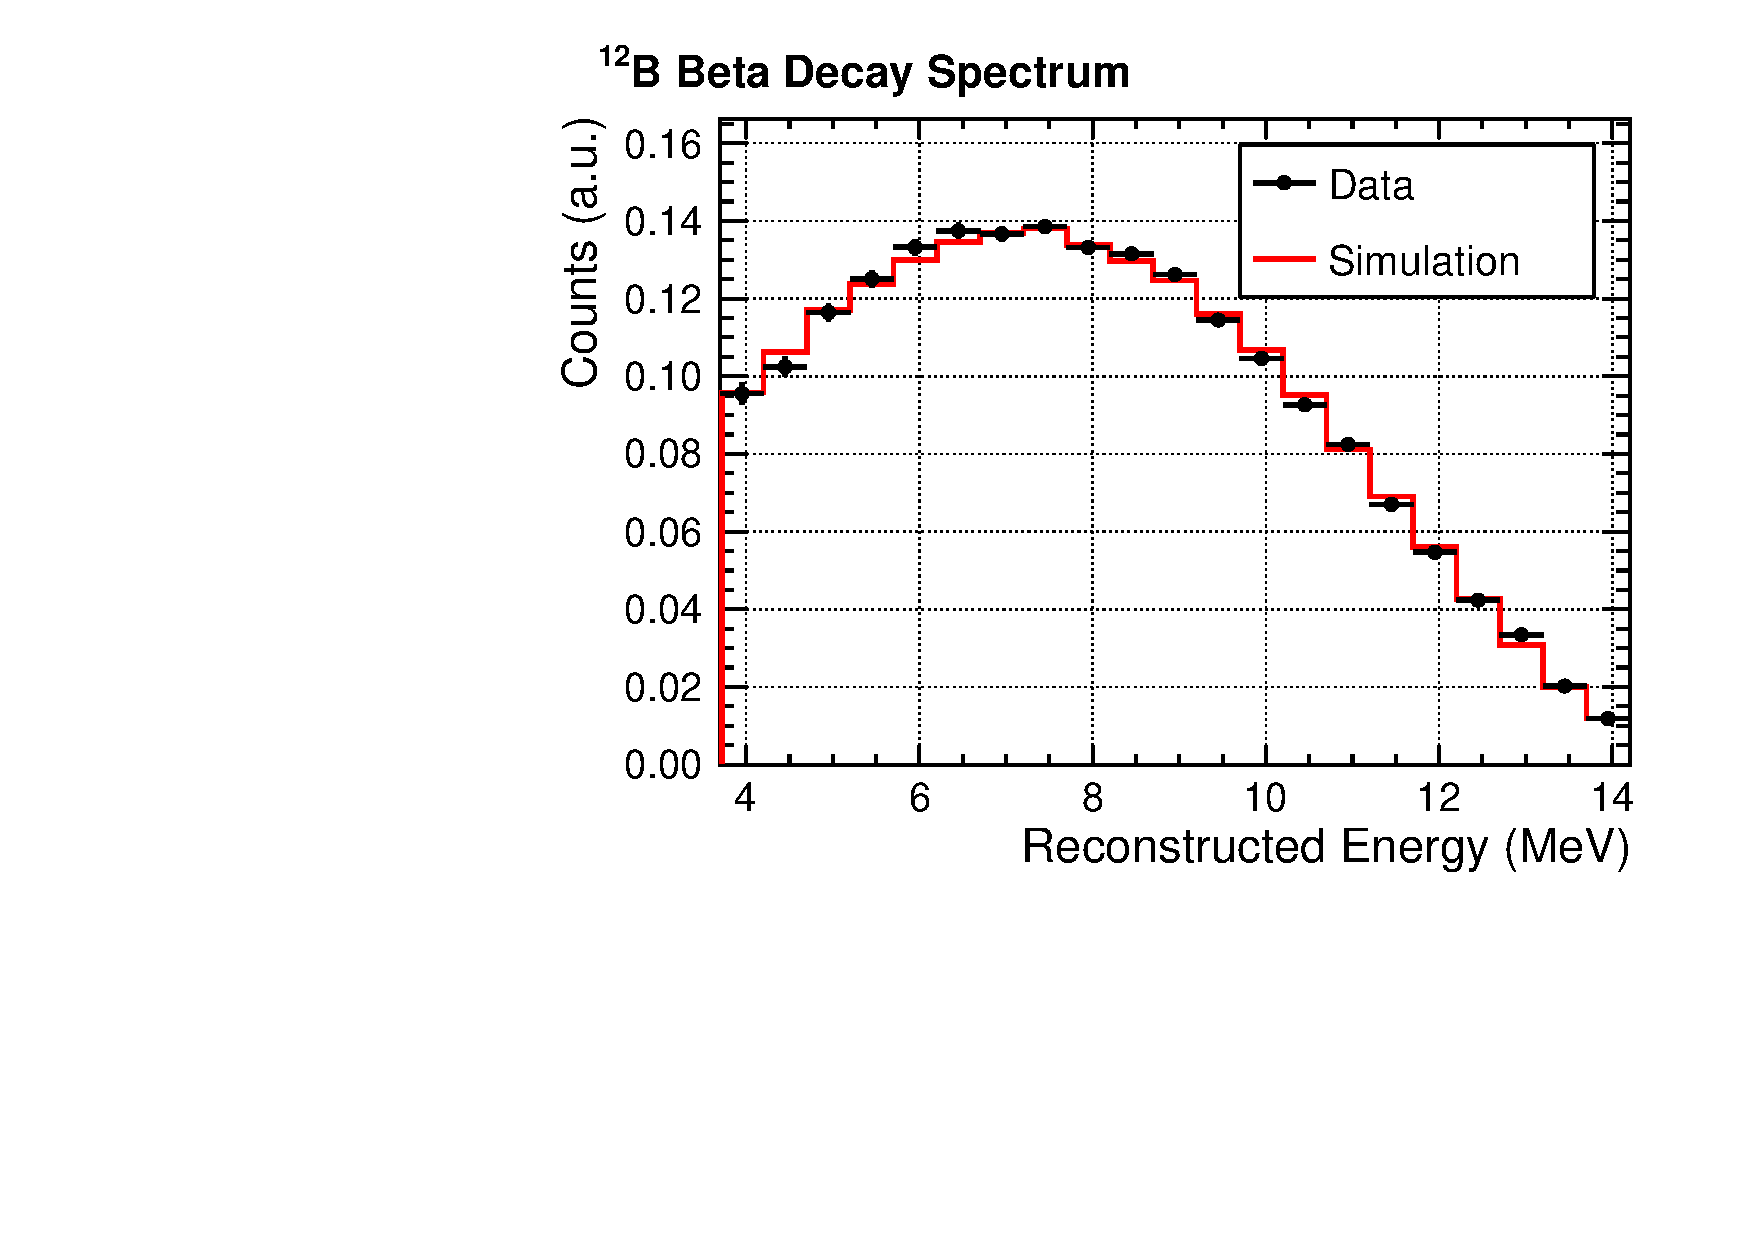
\includegraphics[width=0.75\linewidth]{images/B12_measure_spectrum_v34.pdf}
  \caption[Spectre de décroissance beta du $\ce{^{12}B}$ mesuré pendant la phase 2]{Spectre de décroissance beta du $\ce{^{12}B}$ mesuré pendant la phase 2. L'histogramme en rouge représente les résultats obtenus avec la simulation. L'énergie a été reconstruite avec des coefficients associés à la version 34.}
  \label{fig:B12_measure_spectrum_v34.pdf}
\end{figure}

}

Le spectre électron a été mesuré entre 4 et 16 MeV avec un temps Prompt-Retardé entre 2 et 60 ms. Le taux de comptage mesuré est de $703 \pm 4$ décroissances par jour avec un rapport signal sur bruit allant de 0,1 à 1. Le spectre mesuré dans les données est présenté sur la figure \ref{fig:B12_measure_spectrum_v34.pdf} avec la simulation.\\

À l'heure actuelle, la forme du spectre électron du $\ce{^{12}B}$ est la seule observable nous permettant de contraindre les distorsions de l'échelle en énergie après $\SI{5}{MeV}$. Cet apport est essentiel pour délibérer sur la présence ou non du \og Bump \fg{} à $\SI{5}{MeV}$ sur le spectre antineutrino. Des études sont actuellement menées pour quantifier la comparaison de ce spectre avec la simulation \textsc{Geant4} et affiner le bilan d'incertitudes sur la calibration.\\

\bigbreak

\section{Estimation des incertitudes systématiques}
\label{sec:estimation_escale_errors}

Les incertitudes sur l'échelle en énergie sont quantifiées en deux composantes: une corrélée entre cellules et une décorrélée cellule à cellule (les corrélations entre bins d'énergie sont toujours de 100\%). La composante corrélée a pour but d'autoriser une déformation globale sur l'échelle en énergie dont l'amplitude est contrainte par les variations temporelles du pic n-H. La composante décorrélée permet d'appliquer une distorsion sur l'échelle en énergie pour chaque cellule indépendamment des autres. L'évaluation de ces erreurs systématiques est décrite dans les sections suivantes.\\


\subsection{Incertitudes systématiques corrélées entre cellules}

L'évolution des paramètres de collection de lumière est corrigée au premier ordre grâce à la reconstruction en énergie. Cependant, le figure \ref{fig:nX_relative_evol} montre que les variations temporelles qui persistent ne peuvent être expliquées par les barres d'erreur statistiques seules. Le reste du bilan d'erreur est traité comme une systématique commune aux 6 cellules: \og incertitude systématique sur l'échelle en énergie corrélée entre cellules \fg{}.\\

Afin de quantifier sa valeur, une constante ($\sigma^{syst}$) est ajoutée quadratiquement à la barre d'erreur de chaque point. Le niveau de confiance de la déviation par rapport à la moyenne (0) est formalisé avec un $\chi^2$ :

\begin{equation}
    \chi^2 = \sum_{i=\textrm{cellule,date}} \frac{\left(D_i - 0\right)^2}{(\sigma_i^{stat})^2 + (\sigma^{syst})^2}.
\end{equation}

\bigbreak

La valeur de $\sigma^{syst}$ est choisie de façon à ce que le $\chi^2$ réduit ($\chi^2$ divisé par le nombre de degrés de liberté) soit égale à 1. Les valeurs de $\sigma^{syst}$ sont reportées dans la Table \ref{tab:dE_corr}.\\

\begin{table}[h!]
  \begin{center}
    \begin{tabular}{|c|c|c|c|}
      \hline
      Phase & \'Evolution en temps & Décalage n-H & Total\\
      \hline
      1 & $\pm 0.4 \%$ & $\pm 1.0 \%$ & $\pm 1.1 \%$\\
      \hline
      2 & $\pm 0.3 \%$ & $\pm 1.0 \%$ & $\pm 1.0 \%$ \\
      \hline
    \end{tabular}
  \end{center}
  \caption{Erreurs systématiques liées à l'évolution relative de l'échelle en énergie.}
    \label{tab:dE_corr}
\end{table}

\bigbreak

À cause du décalage de $+1\%$ du pic hydrogène dans la simulation, une autre composante est ajoutée dans le Tableau \ref{tab:dE_corr}. La systématique totale est finalement obtenue en faisant la somme quadratique des deux termes.\\

Les déformations du spectre positron engendrées par ce paramètre commun sont décrites par un paramètre de nuisance, dont la variation est contrainte par la valeur de l'incertitude. Cet aspect est approfondi dans la Section \ref{seq:incert_propag}.

\bigbreak

\subsection{Incertitudes systématiques non corrélées entre cellules}

Puisque les dépôts d'énergie des gammas de $\SI{2.2}{MeV}$ engendrés par les neutrons cosmogéniques sont similaires à ceux des neutrinos, les écarts observés sur le pic n-H offre un moyen d'estimer l'erreur systématique associée à l'ancrage en énergie. L'amplitude des déviations systématiques est estimée en traçant une zone autour de la valeur moyenne à $\pm 1\sigma$ sur la figure \ref{fig:DataMC_diff_Mn_nH_v34.png} (bande bleue). Par ailleurs, les résidus sur l'ancrage ($E^\textrm{ref}$) sont propagés dans cette composante. Les valeurs sont répertoriées dans la Table \ref{tab:dE_uncorr}. \\

\begin{table}[h!]
  \begin{center}
    \begin{tabular}{|c|c|c|c|}
      \hline
      Phase & Dispersion n-H & Résidus ancrage & Total\\
      \hline
      1 & $\pm 0.5 \%$ & $\pm 0.2 \%$ & $\pm 0.5 \%$\\
      \hline
      2 & $\pm 0.5 \%$ & $\pm 0.2 \%$ & $\pm 0.5 \%$\\
      \hline
    \end{tabular}
  \end{center}
  \caption{Erreurs systématiques liées à l'ancrage n-H.}
    \label{tab:dE_uncorr}
\end{table}


\bigbreak

Lors de l'analyse des spectres neutrino, un paramètre de nuisance est associé à chaque cellule. Chaque paramètre est indépendant des autres, et entraine la déformation du spectre neutrino d'une cellule. L'amplitude des déformations est contrainte par la valeur des incertitudes de la Table \ref{tab:dE_uncorr}.


% \subsection{Contraintes des non-linéarités sur l'échelle en énergie}

% Quenching

%\section{Observations et discussion}
%
%\begin{itemize}
%    \item Difficultés techniques
%    \item effets résiduels
%    \item Besoin de meilleures contraintes à hautes énergie
%\end{itemize}

% Difficulties
% modèle de birks > step length bug
% mismatch Qtot Full after tuning quenching
